\documentclass[12pt]{article}
\usepackage[margin=1in]{geometry}
\usepackage{lmodern}
\usepackage{amsmath,amssymb,amsthm,mathtools}
\usepackage{booktabs,threeparttable,graphicx,setspace,enumitem,longtable,array,tabularx}
\usepackage{xcolor}
\usepackage{etoolbox}
\AtBeginEnvironment{tabular}{\footnotesize}
\usepackage[authoryear,round]{natbib}
\usepackage[colorlinks=true,linkcolor=blue!50!black,citecolor=blue!50!black,urlcolor=blue!50!black]{hyperref}
\usepackage{fancyhdr}
\onehalfspacing
\emergencystretch=2em
\pagestyle{fancy}\fancyhf{}
\fancyhead[L]{\small Niroula, Niroula and Khatiwada}
\fancyhead[R]{\small A Sufficient Statistic for Algorithmic Feedback}
\fancyfoot[C]{\thepage}
\renewcommand{\headrulewidth}{0.3pt}
\setlength{\headheight}{14pt}

\newtheorem{theorem}{Theorem}[section]
\newtheorem{proposition}[theorem]{Proposition}
\newtheorem{lemma}[theorem]{Lemma}
\newtheorem{corollary}[theorem]{Corollary}
\theoremstyle{definition}
\newtheorem{definition}[theorem]{Definition}
\newtheorem{assumption}[theorem]{Assumption}
\theoremstyle{remark}
\newtheorem{remark}[theorem]{Remark}
\newcommand{\E}{\mathbb{E}}
\newcommand{\R}{\mathbb{R}}
\newcommand{\KL}{D_{\mathrm{KL}}}
\newcommand{\lab}[1]{}
\title{A Sufficient Statistic for Algorithmic Feedback:\\ What Prices Reveal About Trader Groups, and Who Needs the Rest}
\author{Pratik Niroula\thanks{Department of Computer Information Science, Minnesota State University, Mankato, MN 56001, USA. \texttt{pratik.niroula@mnsu.edu}.}
\and Prashant Niroula\,\thanks{Faculty of Management, Tribhuvan University, Kirtipur, Nepal. \texttt{prashantniroula20@gmail.com}.}
\and Sujan Khatiwada\thanks{Department of Electrical, Computer and Robotics Engineering, Minnesota State University, Mankato, MN 56001, USA. \texttt{sujan.khatiwada@mnsu.edu}.}}
\date{Working paper, core version: 11 November 2026}

\usepackage{array}
\makeatletter\g@addto@macro\UrlBreaks{\do\_}\makeatother
\begin{document}
\maketitle
\thispagestyle{empty}
\begingroup\onehalfspacing

\begin{abstract}
\noindent In a market with algorithmic feedback traders, the feedback kernel---the response of total feedback flow to past prices---is a sufficient statistic for aggregate dynamics. For any insider and causal dealer rule, populations with the same kernel generate identical prices, profits, and equilibria, and public prices identify nothing finer. Learning group composition costs the known $(\Delta\eta)^{-(4K-2)}$ mixture rate, which survives the closed loop and holds in an inventory equilibrium. Position limits introduce a second layer: a capacity measure over memory and leverage. Calm markets reveal only the linear kernel, carrying zero information about proximity to hard limits. Probes large enough to reach the limits identify the net capacity at each memory and leverage. In a pre-registered out-of-sample test on Taiwan's tagged exchange flows (2019--2023), prices improve forecasts of foreign investors' flow as the registered criterion requires, but a pre-specified check attributes the gain to prices revealing past flow rather than to feedback. Core statements are machine-checked in Lean~4.
\end{abstract}

\noindent\textbf{AI-use disclosure.} Claude, ChatGPT/Codex and Gemini provided material assistance with research development, code, numerical checks, manuscript drafting and internal critique, including the restructuring of this core version. Claude and ChatGPT/Codex developed and checked Lean proofs. Human authors remain responsible for verifying the content and its scholarly contribution before submission. AI checks do not constitute independent review.

\noindent\textbf{Relation to the full working paper.} This is a shortened version, organized around one result. Every result stated here also appears in the full working paper (``What Prices Cannot Tell a Market Supervisor'', 5 November 2026), with the same proof. The exceptions are Proposition~\ref{prop:anylinear}, Proposition~\ref{prop:hiding}, Supplement~\ref{app:everyK} and all of Section~\ref{sec:saturating}, which are new to this version and have not appeared elsewhere. The full working paper calls the trader groups ``co\-horts''. Results not needed for the main argument are omitted, among them account-level capital, general memory, spectral blindness and the empirical tests, which this version only summarizes. Section~\ref{sec:scope} says where they are.

\noindent\textbf{Keywords:} algorithmic trading, feedback trading, sufficient statistics, aggregation, identification, market microstructure, supervision, disclosure.\\
\textbf{JEL:} C32, D83, G14, G18.

\noindent\textbf{Code and proofs.} All code, Lean proofs and result files are public at \url{https://github.com/Pratikn03/Fianince}.

\endgroup
\newpage
\setcounter{page}{1}

\section{Introduction}\label{sec:intro}

Much of today's trading is done by programs that read recent prices, decide what to trade, and by trading move the prices they read. Trend-following funds, execution algorithms, market-making programs and, more recently, AI trading agents all work this way. When such a market misbehaves, supervisors ask who was trading and how fast those traders react. This paper asks a prior question: what does a market's price record reveal about its population of feedback traders, and for which decisions is that enough?

\paragraph{The answer in one sentence.} Prices reveal the market's \emph{feedback kernel}: the response, $m$ periods later, of total feedback flow to a unit move in the price signal. That kernel is all that prices identify, and it is all that anyone trading on public information needs. Group composition, meaning who the groups are and how strongly each trades, matters only for actions aimed at a particular group, and learning it from prices has a known and steep price.

\paragraph{The model.} The market has a price and $K$ groups of traders. Each group keeps an exponentially weighted average of past prices, with memory rate $r_i$, and trades in proportion to it with weight $w_i$. A desk that tracks a trend with a Kalman filter, or that learns by regularized online gradient descent, behaves exactly this way (Lemma~\ref{lem:micro}). Total feedback flow is then a convolution of past prices with the kernel
\[
 k_m=\sum_i w_i r_i^{\,m},\qquad m=0,1,2,\ldots,
\]
the moments of the \emph{merged measure} $M$, which puts weight $w_i$ at rate $r_i$. The paper rests on three results about this one object.

\begin{enumerate}[label=(\arabic*),leftmargin=*,itemsep=2pt]
\item \emph{The kernel is sufficient} (Theorem~\ref{thm:eqinv} and Proposition~\ref{prop:anylinear}). Add a value, noise traders, an insider and a dealer, each following an arbitrary causal rule, which covers Kyle, inventory-averse, learning and misspecified dealers. Two trader populations with the same kernel then produce the same price and order-flow paths, the same insider trades and profits and the same dealer inventories, realization by realization. The two games have the same strategy sets and payoffs, and hence the same equilibria. The proof needs only that aggregate feedback flow is a fixed linear function of past public signals, so the result holds for any linear trader population, not only exponential memories.
\item \emph{The kernel is all that prices identify} (Theorem~\ref{thm:merged}). Two populations give identical price responses to every trade sequence if and only if their merged measures coincide. Groups with the same memory cannot be separated however long the record. Groups with different memories can be separated in principle.
\item \emph{Learning more has a known price} (Theorems~\ref{thm:kcohort}, \ref{prop:esprit} and~\ref{prop:passive}). To separate $K$ groups whose memories lie within $\Delta\eta$ of each other takes of order $(\Delta\eta)^{-(4K-2)}$ experiments, and Prony's method attains this order. Waiting instead of trading does not help: passive observation needs at least the same order of observations.
\end{enumerate}

\paragraph{The results survive equilibrium.} In the base model the price impact and the persistence of mispricing are primitives. Section~\ref{sec:equilibrium} derives both from competitive dealers who dislike holding inventory. The equilibrium price is then the same closed loop, path by path, with effective impact and persistence and with the memory rates unchanged (Theorem~\ref{thm:eqreduced}). So the kernel remains the sufficient statistic, and the cost of going beyond it keeps its order. The supplement adds a strategic insider with short-lived information. It also shows that, with positive feedback, liquidity disappears beyond a threshold in dealer risk aversion that falls with the feedback intensity.

\paragraph{What the kernel misses: limits.} Real feedback traders have position limits, margin and risk budgets. Section~\ref{sec:saturating} gives a two-layer theory for traders whose positions saturate.
\begin{itemize}[itemsep=1pt,topsep=2pt]
\item The sufficient object becomes a capacity-weighted measure over memory and leverage, of which the kernel is one linear functional (Theorem~\ref{thm:satsuff}).
\item Calm-market prices reveal the kernel and nothing more. Under hard limits, two populations with the same kernel give identical prices until some trader reaches its limit (Theorem~\ref{thm:stress}). Calm data therefore carry no information about how close traders are to their limits, and Gaussian data carry exponentially little. Under smooth limits, the information grows like the sixth power of the probe (Proposition~\ref{prop:smooth}).
\item Stress reveals everything that matters. Responses to probes of all sizes identify the net capacity at every memory and leverage level, which is exactly the equivalence class (Theorem~\ref{thm:satident}).
\item The results extend to traders who deleverage or liquidate outside their bands (Proposition~\ref{prop:delever}). An informed dealer who prices next-period flow leaks leverage information into calm prices, but only at the scale of the probability of a breach (Proposition~\ref{prop:dealers}).
\end{itemize}

\paragraph{Supervision splits in two.} A market-wide action, such as a uniform cut in activity to meet a ceiling on the feedback budget, depends on the population only through the kernel. A targeted action, such as halting the largest group, does not. Two populations whose price responses differ only by order $(\Delta\eta)^3$ can need different halts (Proposition~\ref{prop:target}). For such decisions, flow reported separately by trader class turns each group into an ordinary regression, with no penalty as the groups' memories approach each other (Proposition~\ref{prop:tagged}). It cuts the number of experiments needed by a factor of order $(\Delta\eta)^{-(4K-2)}$ (Theorem~\ref{thm:discvalue}).

\subsection{What is known and what is new}\label{sec:lit}

The central idea of this paper, that an aggregate is determined by a distribution of individual coefficients and not by the individuals, is old. We state its precedents first, because they fix what we can claim.

\paragraph{Aggregation of dynamic models.} \citet{granger1980} showed that aggregating many first-order autoregressions with different coefficients produces a process whose dynamics are governed by the distribution of the coefficients; with enough mass near one the aggregate has long memory. \citet{zaffaroni2004} develops the theory for large economies. Recovering the coefficient distribution from aggregate data is known as the disaggregation problem \citep{celov2008}. Our merged measure $M$ plays the role of that coefficient distribution, and Theorem~\ref{thm:merged}(i) is the corresponding identification statement for a closed feedback loop. \citet{forni1997} develop the general theory of what aggregate dynamics reveal about heterogeneous individual dynamics, and \citet{pesaran2014} the large-panel version.

\paragraph{Sufficient statistics for aggregate dynamics.} In macroeconomics, \citet{auclert2024} show that the matrix of intertemporal marginal propensities to consume is a sufficient statistic for the output response to fiscal policy, whatever the household heterogeneity behind it. The kernel $k$ plays the same role for a market with feedback traders. It is the response of aggregate demand to past prices, and it summarizes every heterogeneity that matters for prices.

\paragraph{Observational equivalence.} \citet{sargent1976} showed that two macroeconomic theories with opposite policy implications generate the same reduced form, so that data from one policy regime cannot decide between them. Theorem~\ref{thm:eqinv} is a result of this kind for trader populations, and Section~\ref{sec:supervision} draws the policy consequence: which supervisory actions the equivalence class supports, and which need data from outside it.

\paragraph{Mixture estimation.} The order $(\Delta\eta)^{-(4K-2)}$ is the known minimax rate for finite mixtures with $K$ near-colliding components \citep{heinrich2018,wu2020}, and super-resolution theory gives the same conditioning for clustered exponentials \citep{moitra2015,batenkov2021,katz2023}. We do not claim the exponent.

\paragraph{Heterogeneous horizons under impact.} \citet{leclere2026} study a linear mean-field model in which agents with heterogeneous forecast horizons trade under market impact, and in which impact depends on aggregate positions rather than on trader identities. Their object is equilibrium and price regularity, not what an observer can identify or what supervision needs.

\paragraph{Feedback trading and insiders.} Positive-feedback traders and their effect on prices go back to \citet{delong1990}. \citet{barberis2015,barberis2018} model extrapolators with exponentially weighted memories, and \citet{brock1998} model heterogeneous rules. The insiders and dealers covered by Section~\ref{sec:suff} include those of \citet{kyle1985} and of inventory models in the tradition of \citet{hostoll1981} and \citet{grossman1988}.

\paragraph{What is new.} Five things, each of which uses the market setting.
\begin{enumerate}[label=(\alph*),leftmargin=*,itemsep=2pt]
\item \emph{Sufficiency inside a strategic market.} The aggregation literature concerns the statistical law of an aggregate series. Theorem~\ref{thm:eqinv} is a statement about games: it holds path by path for every insider strategy and every causal dealer rule, so it transfers to every equilibrium concept defined from payoffs and public histories. Part~(iv) shows where it stops, since group-level quantities are not invariant.
\item \emph{Memories are zeros of the closed loop.} In mixture and open-loop problems the unknown rates are locations or poles of the observed law. In a feedback market they are transmission zeros of the price response (Theorem~\ref{thm:minphase}). That decides which estimators are valid: fitting poles to prices finds the closed-loop eigenvalues and misses the memories. Because the closed loop is minimum phase, passive data face at least the same barrier as active probing.
\item \emph{The results hold in equilibrium.} With inventory-averse dealers who price the feedback traders' predictable flow, the equilibrium is still the closed loop, with unchanged memories (Theorem~\ref{thm:eqreduced}).
\item \emph{Limits are invisible until reached, and stress reveals them exactly.} With saturating traders, the sufficient object is a measure over memory and leverage. Calm-market prices reveal only its linear part, and stress identifies all of it (Section~\ref{sec:saturating}). The last step of the stress result rests on a known uniqueness theorem for networks with one hidden layer \citep{sussmann1992}; the reduction from prices to that setting is ours.
\item \emph{A supervisory split with a price.} The kernel suffices for market-wide actions and not for targeted ones, and class-tagged disclosure removes the cost of the targeted information (Propositions~\ref{prop:target} and~\ref{prop:tagged}, Theorem~\ref{thm:discvalue}). A group that can mimic another group's memory also caps what any price-based targeting can achieve, whatever the amount of data (Proposition~\ref{prop:hiding}).
\end{enumerate}
The induction behind Theorem~\ref{thm:eqinv}(iii) is short. Its content is not the induction but the object it isolates. The kernel is identified from prices, it is sufficient for every price-based outcome, and it is insufficient exactly for the targeted decisions supervisors care about.

\paragraph{Machine checking.} The core statements are checked in Lean~4 against Mathlib with standard axioms only. The checks cover the sufficiency theorem (pathwise, for arbitrary causal rules), the $K$-group lower and upper bounds, the minimum-phase identification, the finite-sample passive bound, the reduced form of the inventory equilibrium, and the reduced form and best response in the insider equilibrium. Each statement says what is checked and what is proved only on paper; Supplement~\ref{app:verification} lists the declarations.

\paragraph{Outline.} Section~\ref{sec:model} sets out the model. Section~\ref{sec:suff} proves that the kernel is sufficient and that it is what prices identify. Section~\ref{sec:equilibrium} shows that both hold in equilibrium. Section~\ref{sec:cost} prices the information beyond the kernel. Section~\ref{sec:supervision} shows which supervisory decisions need it and what disclosure buys. Section~\ref{sec:saturating} turns to saturating traders. Section~\ref{sec:scope} states the limits, and Section~\ref{sec:conclusion} concludes.

\section{Model and motivating examples}\label{sec:model}

\paragraph{The model in words.} The market has one price and $K$ groups of traders. Each period three things happen. First, the price moves: it drifts back toward its fundamental value, and it is pushed by the groups' trades, by any test trade and by news. Second, each group updates its view by mixing the newest price into its running average, with weight $\eta_i$ on the newest price and $1-\eta_i$ on its old view. Third, each group trades in proportion to its view, with intensity $q_i$. A group with a large $\eta_i$ has a short memory and reacts quickly, like a short-horizon trend follower; a group with a small $\eta_i$ has a long memory and reacts slowly. The equations below write this down.

Time is discrete. Let $p_t$ be the price, $p^*$ the fundamental value and $x_t=p_t-p^*$ the pricing error. A reduced-form dealer sector absorbs net order flow with price impact $\kappa>0$, an imposed primitive rather than an equilibrium quote, and arbitrage pulls the error toward zero with persistence $a\in[0,1)$:
\begin{equation}\label{eq:price}
x_t = a x_{t-1} + \kappa \sum_{i=1}^K q_i y_{i,t-1} + \kappa v_t + w_t,
\end{equation}
where $v_t$ is an executed probe quantity and $w_t$ a price innovation. Group $i$ holds a state $y_{i,t}$ with exponential memory and trades $q_i y_{i,t}$:
\begin{equation}\label{eq:cohort}
y_{i,t} = (1-\eta_i)\,y_{i,t-1} + \eta_i x_t,\qquad \eta_i\in(0,1).
\end{equation}
The ordering is \emph{price first}: the price responds to the probe, then groups update. Write $r_i=1-\eta_i$ for the memory rate and $w_i=q_i\eta_i$ for the merged weight. The feedback kernel and its transform are
\begin{equation}\label{eq:kernel}
k_m=\sum_i w_i r_i^{\,m},\qquad G(z)=\sum_i \frac{w_i z}{z-r_i},
\end{equation}
and the transfer function from probes to prices, $H(z)=\sum_{j\ge0}h_jz^{-j}$, is
\begin{equation}\label{eq:H}
H(z)=\frac{\kappa z}{z-a-\kappa G(z)}=\frac{\kappa zD(z)}{(z-a)D(z)-\kappa N(z)},\qquad G=\frac ND,\quad D(z)=\prod_{i}(z-r_i),
\end{equation}
with impulse response $h_0=H(\infty)=\kappa,h_1,h_2,\ldots$; in particular $H(1)=\sum_jh_j=\kappa/(1-S)$, where $S=a+\kappa\sum_iq_i$ is the feedback budget. Stacking $z_t=(x_t,y_{1,t},\ldots,y_{K,t})^\top$ gives $z_t=Jz_{t-1}+bv_t$, where, because groups update on the same period's price, the probe enters every state on impact through
\begin{equation}\label{eq:b}
b=\kappa\,(1,\eta_1,\ldots,\eta_K)^\top ,
\end{equation}
and
\begin{equation}\label{eq:J}
J=\begin{pmatrix} a & \kappa q_1 & \cdots & \kappa q_K\\ \eta_1 a & 1-\eta_1+\eta_1\kappa q_1 & \cdots & \eta_1\kappa q_K\\ \vdots & & \ddots & \vdots\\ \eta_K a & \eta_K\kappa q_1 & \cdots & 1-\eta_K+\eta_K\kappa q_K\end{pmatrix},\qquad S\equiv a+\kappa\sum_i q_i .
\end{equation}
In the \emph{positive economy} ($q_i\ge0$), $J$ is entrywise nonnegative, its price row sums to $S$, and the economy is Schur stable iff $S<1$.

\begin{lemma}[Two motivating examples: filtering and learning]\label{lem:micro}
\begin{enumerate}[label=(\roman*)]
\item \emph{Kalman memory.} A desk that tracks a latent random-walk trend $v_{t+1}=v_t+\zeta_{t+1}$, $\zeta\sim N(0,\sigma_\zeta^2)$, from signals $r_t=v_t+\nu_t$, $\nu\sim N(0,\sigma_\nu^2)$, using the steady-state Kalman filter, updates as $\hat v_{t+1}=(1-\eta)\hat v_t+\eta r_t$ with
\begin{equation}\label{eq:kgain}
\eta=\frac{-\sigma_\zeta^2+\sqrt{\sigma_\zeta^4+4\sigma_\zeta^2\sigma_\nu^2}}{2\sigma_\nu^2}\in(0,1).
\end{equation}
\item \emph{Gradient memory.} Online gradient descent with $L_2$ regularization $\gamma\in(0,1)$, step size $\alpha>0$ and loss $\tfrac12H(x_t-\theta_t)^2$ gives $\theta_{t+1}=(1-\eta)\theta_t+\eta q x_t$ with $\eta=\gamma+\alpha H\in(0,1)$ and $q=\alpha H/\eta$. A tabular value update with learning rate $\eta$ at a fixed state has the same form; general reinforcement-learning policies need not.
\end{enumerate}
\end{lemma}

\paragraph{Why exponential memory, and what is assumed.} Exponential memory is the oldest model of expectations in economics: adaptive expectations \citep{cagan1956,nerlove1958} and geometric distributed lags \citep{koyck1954}, and \citet{muth1960} showed that exponentially weighted forecasts are optimal for a random walk observed with noise, which is Lemma~\ref{lem:micro}(i). Lemma~\ref{lem:micro} shows that two different design philosophies, Bayesian filtering and regularized online learning, produce the same reduced-form state. A third example is a desk that each period trades the amount that maximizes $\hat v_tu-\tfrac12(\kappa+\lambda)u^2$, a one-period trade-off between its trend forecast $\hat v_t$ and quadratic impact and holding costs. Its trade is $u_t=\hat v_t/(\kappa+\lambda)$. If the forecast is updated exponentially, $\hat v_{t+1}=(1-\eta)\hat v_t+\eta x_t$, the trade follows the same recursion, $u_{t+1}=(1-\eta)u_t+wx_t$ with $w=\eta/(\kappa+\lambda)$. This is a static first-order condition, not a dynamic optimum. In these families the memory rate is a known function of a tuning parameter, the desk's signal-to-noise ratio, its regularization or its cost parameters. That is the private information a supervisor would like to recover, although real algorithms need not belong to any of these families. Applied to the pricing error, a desk that cannot separate fundamental news from transitory deviations treats recent deviations as a persistent trend, which is the exponential extrapolation of \citet{barberis2015,barberis2018}. Nothing in the model says such trading is profitable.

The results use six modelling choices: linearity; price-first timing within a period; exponential memory (needed for the identification result, Theorem~\ref{thm:merged}, and the cost results of Section~\ref{sec:cost}, but not for sufficiency); algorithms that do not change their rules when observed (Proposition~\ref{prop:hiding} relaxes this for one group); known primitives $(a,\kappa)$; and stated observation contracts. Unknown primitives can only enlarge the set of candidate populations, so the lower bounds remain valid; Corollary~\ref{cor:unknown_primitives} in the supplement shows that estimating them leaves the upper-bound rate unchanged. Section~\ref{sec:equilibrium} replaces the primitive $(a,\kappa)$ by an equilibrium.

\paragraph{The observer.} The cost results are stated for one observer outside the trader groups: a supervisor, an exchange's surveillance unit or a large desk. It knows $(a,\kappa)$, the law of the observation noise and, for the $K$-group results, $K$. It can \emph{wait}, recording prices driven by natural innovations; \emph{probe}, trading a sequence $v_t$ against the groups from a reset state and recording the response; or \emph{acquire disclosure}, receiving each class's flow. Independent resets are a benchmark that no outside participant can run in a live market. We use them because they make the information content of the data exact. Reset probing is a benchmark for what can be learned, not a proposed policy. Section~\ref{sec:cost} shows separately that passive observation is no cheaper (Theorem~\ref{prop:passive}).

\section{The kernel is a sufficient statistic}\label{sec:suff}

This section states the paper's main result. In a market with an insider, noise traders, a dealer and feedback traders, all following arbitrary causal rules, the feedback traders affect every outcome only through their kernel. The notation for the insider follows \citet{kyle1985}, so in this section $x_t$ is the insider's order, not the pricing error.


\begin{theorem}[The kernel is sufficient]\label{thm:eqinv}
Consider a market with the following participants and rules.
\begin{itemize}[itemsep=1pt,topsep=2pt]
\item A value $v$ and noise trades $z_t$.
\item An insider who submits $x_t=X_t(v,\mathcal H_{t-1})$.
\item A dealer who sets $p_t=P_t(\mathcal H_{t-1},y_t)$ from the public history $\mathcal H_{t-1}$ and the total order flow $y_t=x_t+z_t+f_t$.
\item Feedback groups whose memory states update on a public price statistic $s_t=S_t(p_0,\ldots,p_t)$ by $m_{i,t+1}=r_im_{i,t}+s_t$ from $m_{i,0}=0$, with $r_i=1-\eta_i$ and aggregate flow $f_t=\sum_iw_im_{i,t}$, $w_i=q_i\eta_i$.
\end{itemize}
The rules $X$, $P$ and $S$ are arbitrary causal maps. This covers Kyle, inventory-averse, learning and misspecified dealers, and any insider strategy.
\begin{enumerate}[label=(\roman*),itemsep=1pt]
\item $f_t=\sum_{m<t}k_m\,s_{t-1-m}$, with $k_m=\sum_iw_ir_i^m$, the moments of the merged measure $M$.
\item Two group configurations produce the same aggregate flow on dates $t\le T$ for every signal sequence $(s_t)$ if and only if $k_m=k'_m$ for all $m<T$. On an unbounded horizon this holds if and only if their merged measures coincide. For a fixed signal rule $S$, the `if' direction holds for every price path. The `only if' direction needs a rule that can produce an impulse signal. It fails, for example, for $S\equiv0$, under which every configuration has zero flow.
\item If $k_m=k'_m$ for $m<T$, then for every strategy profile and every realization of $(v,z)$ the following coincide on $t\le T$: the price and order-flow paths, the insider's trades and realized profit, and the dealer's inventory. The two games therefore have the same strategy sets and the same payoff for every profile. They have the same equilibria, with the same outcomes, under any equilibrium concept defined from these payoffs and the public history.
\item Group-level quantities are not invariant. A Gauss and a Radau two-point configuration agree on $k_0,k_1,k_2$, so they are outcome-equivalent for $T=3$, while their largest groups carry weights $\tfrac12$ and $\tfrac34$.
\end{enumerate}
\end{theorem}

\paragraph{In words.} Whatever the insider and the dealer do, two markets whose trader groups have the same merged response produce the same prices, the same order flow and the same insider and dealer outcomes. So the part of the population that prices cannot identify (Theorem~\ref{thm:merged}) is worth nothing to anyone who trades on public information. It matters only for actions aimed at a particular group, such as halting it (Proposition~\ref{prop:target}). Parts (i)--(iv) are machine-checked pathwise for every causal insider, dealer and signal rule (\nolinkurl{Paper1EquilibriumInvariance.lean}). Supplement~\ref{app:eqinv} gives the proof, the unbounded-horizon statement, the extension to group-specific demand shocks and a numerical illustration.

\paragraph{Beyond exponential memory.} The proof of part~(iii) uses only one property of the feedback traders: their aggregate flow is a fixed linear function of past public signals. So the result does not depend on exponential memory.

\begin{proposition}[Any linear population]\label{prop:anylinear}
In the market of Theorem~\ref{thm:eqinv}, replace the groups by any finite population of feedback traders $j=1,\ldots,J$ whose flows are causal linear functions of the public signal,
\[
 f_{j,t}=\sum_{m<t}\kappa^{(j)}_m\,s_{t-1-m},\qquad \kappa^{(j)}=(\kappa^{(j)}_0,\kappa^{(j)}_1,\ldots)\ \text{arbitrary real sequences},
\]
and write $k=\sum_j\kappa^{(j)}$ for the population's kernel.
\begin{enumerate}[label=(\roman*),itemsep=1pt]
\item Two populations produce the same aggregate flow on dates $t\le T$ for every signal sequence if and only if their kernels agree for $m<T$.
\item If their kernels agree for $m<T$, then for every strategy profile and every realization the price and order-flow paths, the insider's trades and realized profit, and the dealer's inventory coincide on $t\le T$, and the two games have the same equilibria under any equilibrium concept defined from payoffs and the public history.
\item Any decomposition of a kernel into individual kernels is consistent with the same outcomes. Prices, flows and all equilibrium outcomes therefore carry no information about the decomposition beyond $k$.
\end{enumerate}
\end{proposition}

\begin{proof}
(i) Aggregate flow is $f_t=\sum_{m<t}k_ms_{t-1-m}$. If the kernels agree for $m<T$, the flows agree on $t\le T$ for every signal. Conversely, the impulse signal $s_j=\mathbf 1\{j=0\}$ gives $f_{m+1}=k_m$. (ii) The strong induction in the proof of Theorem~\ref{thm:eqinv}(iii) (Supplement~\ref{app:eqinv}) uses only that $f_t$ is the same function of the signals before $t$ in both markets, which is part~(i). (iii) follows from (ii), since outcomes depend on the population only through $k$.
\end{proof}

\paragraph{What the exponential case adds.} For general linear traders, nothing about composition beyond $k$ can be learned from anything that prices determine, because any split of $k$ is observationally equivalent. Exponential memory is the case in which more can be learned, and the rest of the paper prices it. Then $k_m=\int r^m\,dM(r)$ is a moment sequence, and the kernel determines the merged measure $M$ (Theorem~\ref{thm:eqinv}(ii) on an unbounded horizon). A finite record determines only finitely many moments, which is why separating close groups is costly. Proposition~\ref{prop:anylinear} is machine-checked for arbitrary kernels (\texttt{p1\_anylinear\_iff}, \texttt{p1\_anylinear\_invariance}); the passage to equilibria is on paper, as in Theorem~\ref{thm:eqinv}.

\paragraph{The analogy with aggregate demand.} The kernel is the response of aggregate feedback demand to past prices. \citet{auclert2024} show that the analogous object for households, the matrix of intertemporal marginal propensities to consume, is a sufficient statistic for the transmission of fiscal policy. In the same way, $k$ summarizes every heterogeneity among feedback traders that matters for prices. The merged measure is the distribution of individual autoregressive coefficients that governs an aggregate in \citet{granger1980}. Two points distinguish the market version. Sufficiency holds inside a game with an insider and a dealer, not only for the law of an aggregate series. And as part~(iv) of Theorem~\ref{thm:eqinv} shows, it fails for group-level quantities, which matter for targeted supervision (Section~\ref{sec:supervision}).

\subsection{What prices identify}

Theorem~\ref{thm:eqinv} says that populations with the same kernel cannot be told apart by anything that price-based trading determines. The converse is that prices determine the kernel. In the probing experiment of Section~\ref{sec:model}, the response of prices to trades is a fixed function of $(a,\kappa,k)$, and it determines the merged measure.


\begin{theorem}[Merged rate--weight equivalence]\label{thm:merged}
Let $\kappa>0$ and $a\in[0,1)$ be known. Use zero initial states and a common probe contract, and observe the modeled price state $x_t$.
\begin{enumerate}[label=(\roman*)]
\item \emph{Equivalence class.} Two economies $\mathcal E^A=\{(q_i^A,\eta_i^A)\}$ and $\mathcal E^B=\{(q_j^B,\eta_j^B)\}$ produce identical price responses for every probe sequence if and only if their merged measures coincide:
\begin{equation}\label{eq:merged}
\sum_{i:\eta_i^A=\eta} q_i^A\eta \;=\; \sum_{j:\eta_j^B=\eta} q_j^B\eta\qquad\forall\eta\in(0,1].
\end{equation}
Write $a'=a+\kappa M(\{0\})$, so that groups with $\eta=1$ (rate $0$) act as part of the anchor. For $a'\neq0$ the minimal realization has dimension $1+|\mathrm{supp}(M)\cap(0,1)|$, counting distinct positive rates with nonzero merged weight after signed cancellation; for $a'=0$ the price carries no state of its own and the dimension is $|\mathrm{supp}(M)\cap(0,1)|$. A group with $\eta=1$ merges into the anchor $a$ without adding a pole.
\item \emph{Separation complexity under average power.} Consider testing a single group with rate $\bar\eta$ against two groups with rates $\bar\eta\pm\delta$ and the same total weight, on a compact family that is uniformly Schur stable with all rates in $[\epsilon,1-\epsilon]$ for some $\epsilon>0$. Observe $\tilde x_t=x_t+\nu_t$ with $\nu_t\sim N(0,\sigma_\nu^2)$ and use deterministic probes with $\frac1T\sum_{t<T}v_t^2\le P$. Any test with worst-case error at most $\alpha\in(0,1/4)$ needs
\begin{equation}\label{eq:Tpower}
T\;\ge\;\frac{4\sigma_\nu^2(1-2\alpha)^2}{C_{\mathcal F}^2P\,\delta^4}=\Omega(\delta^{-4}),
\end{equation}
where $C_{\mathcal F}$ depends only on the family, through $\epsilon$, the bound on $|H|$ implied by uniform stability, and the total weight $q$.
\end{enumerate}
\end{theorem}

\paragraph{In words.} If two trading desks update on prices with the same memory, no amount of price data can tell them apart or say how much each trades: prices reveal only how much trading happens at each memory speed. Desks with different memories can be told apart in principle, and the rest of the paper prices how hard that is.


The memory rates are poles of $G$ and \emph{zeros} of $H$, not closed-loop poles. This has a practical consequence verified in the full working paper: pole-fitting methods applied directly to the price impulse response recover closed-loop eigenvalues ($0.4256$ and $0.8224$ for $K=1$, $\eta=0.3$, $a=0.5$, $\kappa=0.8$, $q=0.2$) and miss the memory rate $0.70$.
\begin{remark}[Scope]\label{rem:scope}
The result concerns the stated model and observation contract. Groups sharing an exact rate enter prices through their merged weight; this does not determine identities or wealth allocations. Nearby rates can be distinguishable with enough information. The $\delta^{-4}$ statement in (ii) is a lower bound on a declared family, with family-dependent constants. A group may choose its rate strategically. The observer then still sees only the merged measure of the rules in use; Proposition~\ref{prop:hiding} draws the consequence.
\end{remark}
\section{Sufficiency and identification in equilibrium}\label{sec:equilibrium}

The identification results of Section~\ref{sec:suff} take the price impact $\kappa$ and the persistence $a$ of pricing errors as given. This section derives both from dealers who dislike holding inventory. It shows that the equilibrium price is the closed loop of Section~\ref{sec:model} with effective parameters and unchanged memory rates. So the kernel stays the sufficient statistic in equilibrium, and the cost of going beyond it (Section~\ref{sec:cost}) keeps its order.


\paragraph{An inventory equilibrium.}
\begin{itemize}[itemsep=1pt,topsep=2pt]
\item \emph{Fundamental and price.} The fundamental $F_t$ is a public random walk with innovation variance $\sigma_F^2$, and the price is $p_t=F_t+x_t$.
\item \emph{Groups.} They trade $u_{i,t+1}=r_iu_{i,t}+w_ix_t$, the paper's exponential memory with $w_i=q_i\eta_i$ and $r_i=1-\eta_i$.
\item \emph{Exogenous flow.} $\xi_t\sim N(0,\sigma_\xi^2)$, i.i.d., stands for noise trades or the observer's probe. Customer flow is $y_t=\sum_iu_{i,t}+\xi_t$.
\item \emph{Dealers.} Competitive dealers absorb the flow and lay off a share $1-\bar a$ of their inventory each period, so $H_t=\bar aH_{t-1}-y_t$. Each overlapping generation of dealers has CARA risk aversion $A$ and holds $H_t$ to the next date: $H_t=(E_tp_{t+1}-p_t)/(AV)$, with $V=\mathrm{Var}_t(p_{t+1})$.
\end{itemize}
We study stationary equilibria in which $x_t$ is linear in the dealers' inventory and the groups' next trades. Write $G(D)=\sum_iw_i/(D-r_i)=\int dM(r)/(D-r)$ for the Stieltjes transform of the merged measure.

\begin{theorem}[Price impact and persistence in an inventory equilibrium]\label{thm:inventory}
Consider stationary linear equilibria of the model above.
\begin{enumerate}[label=(\roman*),itemsep=1pt]
\item \emph{Characterization.} The price law
\[
 x_t=-\kappa H_t+\kappa\sum_i\frac{u_{i,t+1}}{D-r_i}
\]
with $D\ne0$ and $D\ne r_i$, is an equilibrium exactly when the induced dynamics are stable and
\begin{equation}\label{eq:inventory_eq}
 D=1-\kappa\,G(D),\qquad \kappa(D-\bar a)=A\,V\,D,\qquad V=\sigma_F^2+\frac{\kappa^2\sigma_\xi^2}{D^2}.
\end{equation}
An unexpected unit of flow moves the price by $\kappa/D$.
\item \emph{No feedback.} Then $D=1$ and the price law is exactly the paper's $x_t=\bar a\,x_{t-1}+\kappa\,y_t$. The persistence of pricing errors is the dealers' carry share, $a=\bar a$, and the impact $\kappa$ solves $\kappa(1-\bar a)=A(\sigma_F^2+\kappa^2\sigma_\xi^2)$. An equilibrium exists if and only if $\Delta=(1-\bar a)^2-4A^2\sigma_F^2\sigma_\xi^2\ge0$. When $\Delta>0$ there are two, $\kappa_\pm=\bigl((1-\bar a)\pm\sqrt\Delta\bigr)/(2A\sigma_\xi^2)$; the low-impact one $\kappa_-\approx A\sigma_F^2/(1-\bar a)$ is the price of dealer inventory risk.
\item \emph{Invariance.} The coefficients $(\kappa,D,V)$, and hence the price process, depend on the groups only through $G$, and so only through the merged measure $M$. This is Theorem~\ref{thm:eqinv} in equilibrium form.
\item \emph{Small feedback.} Let $\Delta>0$, fix $\delta>0$ with $\max_ir_i<1-\delta$, and let $\epsilon=\sup_{|D-1|\le\delta}(|G(D)|+|G'(D)|)$ be small. Then there is a unique equilibrium near $(\kappa_-,1)$. With $G(1)=\sum_iq_i$, the aggregate feedback intensity,
\[
 D=1-\kappa_-G(1)+o(\epsilon),\qquad \kappa=\kappa_-+\frac{\kappa_-^2(\bar a+2A\kappa_-\sigma_\xi^2)}{\sqrt\Delta}\,G(1)+o(\epsilon).
\]
Positive feedback raises the impact $\kappa$, and it raises the impact of an unexpected flow shock, $\kappa/D$, by more.
\end{enumerate}
\end{theorem}

\paragraph{In words.} Dealers set the price impact and the persistence of mispricing. Impact is what they charge for carrying inventory risk; persistence is how slowly they lay that inventory off. Without feedback traders, this equilibrium is exactly the closed loop the paper starts from. Feedback traders enter only through their merged measure, as Theorem~\ref{thm:eqinv} requires. Positive feedback raises price impact, and dealers price their predictable future trades in advance (the terms in $u_{i,t+1}$). Feedback trading also makes liquidity fragile, not only more expensive: beyond a threshold in dealer risk aversion that falls with the feedback intensity, no equilibrium exists (Theorem~\ref{thm:fragility}).

\paragraph{Machine check.} See Supplement~\ref{app:mc}.

\paragraph{The identification results hold in equilibrium.} With feedback, dealers price the groups' predictable trades in advance, so the response of prices to flow is no longer the reduced form of Section~\ref{sec:model} with the primitive $(a,\kappa)$. The next theorem shows that it is still that closed loop, exactly and path by path, with new parameters and the same memory rates.

\begin{theorem}[The equilibrium is the paper's closed loop]\label{thm:eqreduced}
Take an equilibrium of Theorem~\ref{thm:inventory} with $D\ne\bar a$, and set
\[
 a^*=\frac{\bar a}{D},\qquad \kappa^*=\frac{\kappa}{D},\qquad \tilde w_i=\frac{D-\bar a}{D-r_i}\,w_i .
\]
\begin{enumerate}[label=(\roman*),itemsep=1pt]
\item \emph{Reduced form, pathwise.} Let $\tilde u_{i,t}=\frac{D-\bar a}{D-r_i}u_{i,t}$. For every realization, every initial state and every $t$,
\[
 x_t=a^*x_{t-1}+\kappa^*\Bigl(\xi_t+\sum_i\tilde u_{i,t}\Bigr),\qquad \tilde u_{i,t+1}=r_i\tilde u_{i,t}+\tilde w_ix_t .
\]
So the price follows the closed loop \eqref{eq:price}--\eqref{eq:cohort} with persistence $a^*$, impact $\kappa^*$, exogenous flow $\xi$ in place of the probe, and groups with the same memory rates and merged weights $\tilde w_i$. Its transfer function from flow to price is \eqref{eq:H} with $(a^*,\kappa^*,\tilde w)$. The equilibrium is stable if and only if this closed loop is.
\item \emph{Zeros.} For $\bar a>0$, distinct rates in $(0,1)$ and nonzero weights, the memory rates are the transmission zeros of the equilibrium price response, and none cancels (Theorem~\ref{thm:minphase}(i) with the effective parameters).
\item \emph{Boundary.} The effective merged measure is $\tilde M=h\,M$, where $h(r)=(D-\bar a)/(D-r)$ is positive. The effective parameters determine the equilibrium ones: $D=1-\kappa^*\tilde M([0,1])/(1-a^*)$, $\bar a=a^*D$ and $\kappa=\kappa^*D$. So the merged measure remains exactly what equilibrium prices identify (Theorem~\ref{thm:merged}).
\item \emph{The rates survive.} Let $(a^*,\kappa^*,W,r_c,\Delta\eta)$ satisfy the hypotheses of Theorem~\ref{thm:kcohort} with $(a,\kappa)=(a^*,\kappa^*)$. Then the two $K$-group economies of that theorem are the price responses of two inventory equilibria with identical primitives $(A,\sigma_F^2,\sigma_\xi^2,\bar a)$ and identical $(\kappa,D)$:
 \begin{itemize}[itemsep=1pt,topsep=2pt]
 \item $D=1-\kappa^*W/(1-a^*)$, which exceeds every rate;
 \item $\bar a=a^*D$ and $\kappa=\kappa^*D$;
 \item any $\sigma_F^2,\sigma_\xi^2>0$, with $A=\kappa^*D(1-a^*)/(\sigma_F^2+\kappa^{*2}\sigma_\xi^2)$;
 \item group weights $w_i=\tilde w_i(D-r_i)/(D-\bar a)>0$.
 \end{itemize}
 Hence an observer of equilibrium prices who knows the primitives needs $N\ge c\,\sigma^2(\Delta\eta)^{-(4K-2)}$ experiments. Theorem~\ref{prop:esprit} applies to the effective parameters, and the true weights follow from the effective ones by a Lipschitz map. So $N^*\asymp\sigma^2(\Delta\eta)^{-(4K-2)}$ in equilibrium.
\end{enumerate}
\end{theorem}

\paragraph{In words.} Dealers' anticipation does not hide the groups and does not move them. It replaces the persistence and impact by $\bar a/D$ and $\kappa/D$, and it rescales each group's weight by $(D-\bar a)/(D-r_i)$. Because that factor rises with $r_i$, slow-memory groups weigh more in equilibrium prices. The memory rates are untouched.
\begin{itemize}[itemsep=1pt,topsep=2pt]
\item Every result of Sections~\ref{sec:suff} and~\ref{sec:cost} that concerns the map from order flow to prices therefore holds in equilibrium: identification, sample complexity, passive observation, and probing costs computed from the price path. Its constants are evaluated at the effective parameters.
\item The lower-bound pair is not an artefact of the reduced form. Two economies with the same dealers, the same risk aversion and the same impact differ only in their groups, and they are as hard to tell apart as Theorem~\ref{thm:kcohort} says.
\item Part (i), the realization in part (iv) and the effective group recursion are machine-checked (\nolinkurl{Paper1EquilibriumReducedForm.lean}).
\item One assumption is new: the observer's probe is part of the exogenous flow that dealers price as noise. Dealers who recognized a probe would price it differently.
\end{itemize}

\paragraph{Further equilibrium results.} Four results in Supplement~\ref{app:eqinv} extend this section. None is needed for the main argument.
\begin{itemize}[itemsep=1pt,topsep=2pt]
\item \emph{A strategic insider} with short-lived information (Theorem~\ref{thm:insider}). The equilibrium is characterized in closed form and nests Kyle's one-period values. Its coefficients depend on the groups only through $G$, and the observed price is the closed loop driven through a known invertible moving-average filter. So the identification boundary and the $(\Delta\eta)^{-(4K-2)}$ rate hold with an insider present. Positive feedback raises total impact, and the insider then trades less and prices reveal less of her news.
\item \emph{Fragility} (Theorem~\ref{thm:fragility}). With positive feedback, a positive-impact equilibrium exists only if dealer risk aversion lies below a threshold. For strong feedback the threshold is inversely proportional to the feedback intensity $G(1)$. With several groups the bound depends on the population only through $G(1)$, again an aggregate.
\item \emph{Rents} (Theorem~\ref{thm:rents}). A dealer that misjudges the aggregate response by $\varepsilon$ hands an insider with a committed schedule a rent of exact order $\varepsilon$, or charges it one. Public data reveal the aggregate response at the ordinary rate. So the information that protects price formation is cheap to learn.
\item \emph{A targeted halt in equilibrium} (Theorem~\ref{thm:eqhalt}). Two markets that agree in equilibrium to within the cube of the memory spacing can differ at order one after their largest group is halted.
\end{itemize}
Disclosure keeps its value in equilibrium too (Corollary~\ref{cor:eqdisclosure}).

\section{The price of composition}\label{sec:cost}

Prices identify the kernel, and with exponential memory the kernel determines the merged measure. A finite record, however, pins down only finitely many moments of $M$, each with noise. This section asks how much data it takes to recover the groups. The answer is the known rate for finite mixtures. What the market adds is that the memories must first be extracted from a feedback loop, and that waiting is no cheaper than trading.


\subsection{Many unknown groups}

\begin{theorem}[$K$-group two-point lower bound]\label{thm:kcohort}
Fix $K\ge2$, a center $r_c\in(0,1)$, total merged weight $W>0$ and $0<\Delta\eta<\min(r_c,1-r_c)$, so that all rates lie in $(0,1)$, and assume $a+\kappa W/(1-r_c-\Delta\eta)<1$, so that every candidate economy is Schur stable. Each reset experiment observes the noisy taps $h_0,\ldots,h_{T-1}$ with $T\ge2K+1$ ($T=\infty$ allowed), so that the first tap where the two economies below differ, $h_{2K}$, is observed; the bound below uses the full response norm, which dominates any finite prefix. There exist two $K$-group economies with rates in $r_c+\Delta\eta[-1,1]$, positive weights, and merged measures whose moments of order $0,\ldots,2K-2$ coincide while the moment of order $2K-1$ differs by a constant times $(\Delta\eta)^{2K-1}$. Their impulse responses differ by $\|h^A-h^B\|_2\asymp(\Delta\eta)^{2K-1}$, so recovering the weights from $N$ independent noisy reset experiments with worst-case error probability below $1/4$ requires
\[
N\;\ge\;c\,\sigma^2(\Delta\eta)^{-(4K-2)} .
\]
The same requirement holds for the permutation-invariant loss $W_1(\hat M,M)$ between estimated and true merged measures at accuracy $c_KW\Delta\eta$, where $2c_K>0$ is the Wasserstein distance between the two normalized quadrature rules, so no relabelling of atoms escapes it.
\end{theorem}

The two losses have different targets. The weights of the two economies differ by a constant that does not shrink with $\Delta\eta$, so the first statement is about weights at fixed accuracy, which Theorem~\ref{prop:esprit} matches; the Wasserstein statement is about the memory distribution at accuracy proportional to $\Delta\eta$, which the full working paper matches with an upper bound.

The construction uses the $K$-point Gauss and Gauss--Radau rules of the same weight function: both are positive, have $K$ atoms and integrate polynomials of degree $2K-2$ exactly. For $K=2$ it reproduces the order of Theorem~\ref{thm:twocohort}. Numerically, their low moments agree to machine precision and their moment of order $2K-1$ differs by $0.222$, $0.0533$ and $0.0131$ for $K=2,3,4$. The shrinking gap explains why constants deteriorate with $K$ on top of the exponent. The two rules also differ in their largest weight for every $K$ we checked: for $K=2,\ldots,200$ the largest Gauss--Radau weight exceeds the largest Gauss weight, by $0.25$ at $K=2$ and by about $0.79/K^2$ for large $K$ (\nolinkurl{equilibrium/gauss_radau_maxweight.py}). So the argument given for $K=2$ in Proposition~\ref{prop:target} applies to each such $K$. A proof of this comparison for every $K$ is open. The supervisory result needs less: Lemma~\ref{lem:everyK} proves that, for every $K$, some two rules of this kind have different largest weights.

\paragraph{What counts as an experiment.} In Theorem~\ref{thm:kcohort} an experiment is a unit impulse from the reset state whose response is observed with noise of variance $\sigma^2$ per tap. The exponent is the same for any probe design of bounded energy. For any probe $v$ the mean difference between the two economies is at most $\sup_\omega|\Delta\hat H(e^{i\omega})|\,\|v\|_2$, and $\sup_\omega|\Delta\hat H|=O((\Delta\eta)^{2K-1})$ because $\Delta\hat H=z^{-1}\hat H_A\hat H_B\,\Delta G$ with both responses bounded on the circle. Experiments with probe energy $E$ each therefore need $NE\gtrsim\sigma^2(\Delta\eta)^{-(4K-2)}$: a larger probe buys the same information with fewer experiments, and the account-level analysis of the full working paper prices the capital that a larger probe requires. The bound does not cover information obtained without trading against the groups, such as class records (Section~\ref{sec:supervision}).

\begin{theorem}[Matching upper bound for every $K$]\label{prop:esprit}
Fix $K\ge2$, a compact set $\mathcal S\subset\{s\in[-1,1]^K:s_1<\cdots<s_K\}$ of ordered rescaled rates with $\min_{i\ne j}|s_i-s_j|\ge\gamma>0$, and merged weights $w_i\in[\omega_{\min},\omega_{\max}]$ with $\omega_{\min}>0$. Consider the class of $K$-group economies with rates $r_c+\Delta\eta\,s$, $s\in\mathcal S$, and $N$ independent reset experiments, each observing at least the taps $h_0,\ldots,h_{2K}$ with Gaussian noise of variance $\sigma^2$. There are constants $c_0,C>0$ depending only on $(K,\mathcal S,\gamma,\omega_{\min},\omega_{\max},a,\kappa,r_c)$ such that, whenever $\epsilon_N\equiv\sigma N^{-1/2}(\Delta\eta)^{-(2K-1)}\le c_0/\sqrt{\log(4K/\beta)}$, Prony's method applied to the first $2K$ estimated kernel values, with its output atoms listed in increasing order of rate, recovers the weights with
\[
\max_i|\hat w_i-w_i|\;\le\;C\sqrt{\log(4K/\beta)}\;\epsilon_N
\]
with probability at least $1-\beta$. Hence $N=C'\sigma^2(\Delta\eta)^{-(4K-2)}$ experiments suffice for any fixed accuracy and confidence. On any such class that contains the Gauss and Gauss--Radau pair of Theorem~\ref{thm:kcohort} (a rich class), together with that theorem the minimax sample requirement is $N^*\asymp\sigma^2(\Delta\eta)^{-(4K-2)}$.
\end{theorem}

\paragraph{Smaller classes and constants.} On smaller classes the upper bound need not be tight: if the rates are known, for example, two weights need only order $\sigma^2(\Delta\eta)^{-2}$ experiments. For $K$ known clustered rates the requirement is at least of order $\sigma^2(\Delta\eta)^{-2(K-1)}$. A weight perturbation along the $(K-1)$-th finite difference preserves the moments of order $0,\ldots,K-2$ and changes the moment of order $K-1$ by order $(\Delta\eta)^{K-1}$. For $K=3$, the direction $(1,-2,1)$ on rates $r_c-\Delta\eta,r_c,r_c+\Delta\eta$ changes the second moment by $2(\Delta\eta)^2$. This is still far below the unknown-rate order $(\Delta\eta)^{-(4K-2)}$. The constants $c_0$ and $C$ grow quickly with $K$, through the conditioning of the moment map; the theorem gives the order in $\Delta\eta$ for fixed $K$, not a usable constant for large $K$ (in the full working paper our double-precision Prony implementation already fails at $K=4$ on the disclosure grid).
\paragraph{In words.} With $K$ unknown groups whose memories lie within $\Delta\eta$ of each other, the number of experiments needed grows like $(\Delta\eta)^{-(4K-2)}$. For two groups, halving the spread multiplies the data needed by 64; for three groups, by 1{,}024. Theorem~\ref{thm:kcohort} shows that no method does better, and this theorem shows that Prony's method achieves it.

\subsection{Passive data}

\begin{theorem}[Passive identification: minimum phase]\label{thm:minphase}
Consider a stable economy with $0<a<1$, distinct memory rates $0<r_i<1$ and nonzero merged weights.
\begin{enumerate}[label=(\roman*)]
\item The zeros of $H$ are the memory rates $r_i$ together with a structural zero at $z=0$; none cancels against the denominator, and all lie in the open unit disk, so $H$ is minimum phase. The degenerate anchor ($a=0$) and zero-rate cases require the cancellations described in the proof of Theorem~\ref{thm:merged}.
\item Let the price be driven by a single innovation sequence with variance $\sigma_\xi^2>0$, possibly unknown, so that its spectrum is $f(\omega)=\sigma_\xi^2|H(e^{i\omega})|^2/(2\pi)$. Within the class of (i), $f$ determines $\sigma_\xi^2\kappa^2$ and the normalized response $H/h_0$ (recall $h_0=\kappa$); hence it determines the memory rates. If in addition $\kappa$ (or $\sigma_\xi^2$) and $a$ are known, it determines $H$ and, by Theorem~\ref{thm:merged}, the merged measure.
\end{enumerate}
\end{theorem}


The result holds for signed weights (mean-reverting groups): in 1,733 stable random economies with weights of both signs, the nonstructural zeros equalled the memory rates and lay inside the unit disk. With a second independent shock in the groups' memories, the Jacobian of the price spectrum with respect to six model parameters has full rank, with singular values from $34.51$ down to $0.0698$. Passive noise helps identification rather than hindering it.

\begin{theorem}[Passive cost]\label{prop:passive}
Suppose the price is observed passively as the stationary output $x_t=H_\theta(L)\xi_t$ of i.i.d.\ Gaussian innovations $\xi_t\sim N(0,\sigma^2)$, $\sigma^2>0$ known, without observation noise, for $\theta$ in a compact, uniformly Schur-stable family with rates in $[\eta_{\min},\eta_{\max}]\subset(0,1)$, and let $D(\theta_1\|\theta_0)$ be the Kullback--Leibler divergence rate per observation.
\begin{enumerate}[label=(\roman*)]
\item For a single group at $\bar\eta$ against the symmetric pair at $\bar\eta\pm\delta$ with the same total weight, $D=\Theta(\delta^4)$.
\item For the moment-matched two-group economies of Theorem~\ref{thm:twocohort}, $D=\Theta(\tau^2(\Delta\eta)^6)$.
\item For every $K\ge2$, for the $K$-group Gauss and Gauss--Radau economies of Theorem~\ref{thm:kcohort}, $D=\Theta((\Delta\eta)^{4K-2})$.
\end{enumerate}
Hence any test based on $T$ passive observations with worst-case error at most $\alpha<1/4$ needs $T=\Omega(\delta^{-4})$, $T=\Omega(\tau^{-2}(\Delta\eta)^{-6})$ and $T=\Omega((\Delta\eta)^{-(4K-2)})$ respectively, uniformly as the separation shrinks: passive data cost at least the same polynomial order as active probing for every number of groups. For each fixed pair, at fixed type-I error the likelihood-ratio test's type-II error decays at exponential rate $D$ (Stein's lemma), and both errors decay at the Chernoff-information rate, which is of the same order in the separation. So the orders are the right ones. We do not claim that this attainment is uniform as the separation shrinks. All constants depend only on $K$, the stability margin of the family, the rate interval $[\eta_{\min},\eta_{\max}]$, the total weight and the moment-matched construction; they do not depend on $\delta$, $\Delta\eta$ or $T$. In part (ii) $\tau$ is held fixed as $\Delta\eta\to0$. The testing conclusions use a finite-record bound $\KL(P_1^T\|P_0^T)\le C\,T\,\varepsilon^2$, with $\varepsilon$ the leading moment gap ($\delta^2$, $\tau(\Delta\eta)^3$, $(\Delta\eta)^{2K-1}$); the lower bounds on $D$ and the fixed-pair error exponents are separate statements.
\end{theorem}


\paragraph{In words.} Watching the market without trading does not escape the barrier. A passive observer needs at least the same polynomial order of observations as a prober needs experiments; it pays in time rather than in trading losses. Prices recorded with extra measurement noise that is independent of the price are a garbling of the noiseless record, so by the data-processing inequality they carry less information, and the lower bound holds a fortiori.
\paragraph{Machine checks.} The machine checks of Theorems~\ref{thm:kcohort}--\ref{prop:passive} are described in Supplement~\ref{app:mc}.


\paragraph{In executed quantity and money.} For a \emph{known} pair (one group at rate $\eta$ against two at $\eta\pm\delta$ with the same total weight), the information needed can be stated in trades. The executed quantity a prober needs is of exact order $\delta^{-2}$: the two price responses first differ at lag two, by $-\kappa^2q\delta^2$, and a single pulse of size $2\sigma\Phi^{-1}(1-\alpha)/(\kappa^2q\delta^2)$ attains error $\alpha$. The capital a counterparty must post to fill such probes is of order $\delta^{-4}$, because the adverse mark of a probe grows with the square of its size. Halving the difference between two memories therefore quadruples the trading needed and multiplies the capital by sixteen (Theorems~\ref{thm:quantity} and~\ref{thm:cap} and Lemma~\ref{thm:capital}, Supplement~\ref{app:capital}).

\paragraph{Near instability.} Theorem~\ref{prop:passive} is stated on a family that stays uniformly stable. One might hope that the barrier lifts as the market approaches instability, since the loop then amplifies every difference. It does not. What becomes visible is the distance to instability, not the composition.

\begin{proposition}[The barrier does not lift near instability]\label{prop:nearcrit}
Fix $K\ge2$ and the $K$-group Gauss and Gauss--Radau economies $A$ and $B$ of Theorem~\ref{thm:kcohort}, with positive weights, rates in $(0,1)$ and $\kappa>0$. For a margin $\epsilon>0$, choose persistences $a_A(\epsilon)$ and $a_B(\epsilon)$ so that both economies have feedback budget $S=1-\epsilon$, and suppose $a_A(\epsilon),a_B(\epsilon)>0$ for $\epsilon\le\epsilon_0$. Let $D_\epsilon(B\|A)$ be the Kullback--Leibler divergence rate between the stationary price processes driven by i.i.d.\ $N(0,\sigma^2)$ innovations. There is $C$, not depending on $\epsilon$ or $\Delta\eta$, such that
\[
D_\epsilon(B\|A)\ \le\ C\,(\Delta\eta)^{4K-2}\qquad\text{for all }0<\epsilon\le\epsilon_0\text{ and all small }\Delta\eta .
\]
\end{proposition}

\paragraph{In words.} Even as the market approaches a crash, passive prices reveal no more about who is trading than they did in calm conditions, per observation. They reveal more and more about how close the market is to instability: if the two economies share the persistence $a$ instead of the budget, their budgets differ by order $(\Delta\eta)^{2K-1}$, and numerically the divergence rate then grows like $\epsilon^{-1}$. The proof is in Supplement~\ref{app:nearcrit}. Two limits apply. The statement is about the divergence rate per observation; near instability prices are strongly dependent, and a finite-sample bound that is uniform in $\epsilon$ is not proved. And probing does gain near instability: the squared response difference grows like $\epsilon^{-1}$ (numerical, \nolinkurl{research_extension/fragility_reveals}), but probing a market at the edge of instability is not a policy.

\section{Who needs composition, and what disclosure buys}\label{sec:supervision}

By Theorem~\ref{thm:eqinv}, composition is worth nothing to anyone trading on public information. It can still matter to a supervisor whose action is aimed at one group. This section gives a decision in which it does and the disclosure that removes the cost of learning it. It ends with a bound on what price-based targeting can achieve when a group can hide.

\paragraph{A decision in which attribution matters.} A supervisor must keep the feedback budget $S=a+\kappa\sum_iq_i$ below a prudential ceiling $\bar s$. It can either cut all activity uniformly or halt the largest verified class. The target is the feedback budget, not the spectral radius of the state matrix: in an already stable positive economy, imposing $S\le\bar s<1$ is a tighter prudential constraint, not a restoration of stability.


\begin{proposition}[Supervisory separation: market-wide versus targeted intervention]\label{prop:target}
Assume the positive stable model, known $a,\kappa$, and $a<\bar s<1$. Write $q_i=w_i/(1-r_i)$ and $R=S-\kappa\max_iq_i$ for the post-halt feedback budget.
\begin{enumerate}[label=(\roman*),itemsep=1pt]
\item A uniform scale $\theta$ meets the ceiling exactly when $a+\theta(S-a)\le\bar s$. Its largest feasible value is $\theta^*=\min\{1,(\bar s-a)/(S-a)\}$. The identity $S=1-\kappa/\sum_jh_j$ is algebraic; estimating this infinite sum requires a justified tail bound and an observation/noise model. It alone establishes no unconditional parametric learning rate.
\item For $K=2$, the Gauss and Gauss--Radau pair of Theorem~\ref{thm:kcohort} has limiting largest normalized weights $1/2$ and $3/4$. Thus $|S^G-S^R|=O((\Delta\eta)^3)$ and $q^R_{\max}-q^G_{\max}=W/(4(1-r_c))+O(\Delta\eta)$. For sufficiently small spacing, a nonempty interval of ceilings separates their post-halt decisions. For $N$ independent reset records with common Gaussian noise $\sigma^2 I$, both decision errors at most $1/4$ require
\[
 N\ge (2\Phi^{-1}(0.75)\sigma/\|h^G-h^R\|_2)^2
 \ge c\sigma^2(\Delta\eta)^{-6}.
\]
The record horizon and the response norm must be the same on both sides.
\item Tagged-flow estimation under Theorem~\ref{thm:discvalue}, a rate bound away from one, and a fixed nonzero decision margin gives a bounded sample requirement as the spacing shrinks. The target class must be mapped to an executable, verified class label; a largest latent atom alone supplies no such identity.
\end{enumerate}
\end{proposition}
The proof is in Supplement~\ref{app:decisionfull}. Proposition~\ref{prop:targetK} there extends part~(ii) to every $K$, with exponent $4K-2$.

\paragraph{In words.} A uniform cut needs only the kernel, through $S=1-\kappa/\sum_jh_j$, so public prices suffice for it. A halt of the largest group needs that group's weight, which the kernel does not pin down. The two-group populations of Theorem~\ref{thm:kcohort} (the Gauss and Gauss--Radau pair with $K=2$) have feedback budgets within $O((\Delta\eta)^3)$ of each other, but largest groups that differ at order one. So a range of ceilings exists at which halting the largest group meets the ceiling in one population and not in the other. Prices decide between them only with order $(\Delta\eta)^{-6}$ records. The same holds for any number of groups $K$, with order $(\Delta\eta)^{-(4K-2)}$ records (Proposition~\ref{prop:targetK}).

\subsection{What class-tagged disclosure buys}


\begin{proposition}[Tagged flow removes the barrier]\label{prop:tagged}
Let the price $x_t$ be the causal stationary solution of the model driven by i.i.d.\ centred innovations of variance $\sigma_\xi^2\in(0,\infty)$ in a positive, stable economy, with stationary autocovariances $\gamma_x(s)=\sum_\ell c_\ell\lambda_\ell^{|s|}$ ($c_\ell\ge0$, $0\le\lambda_\ell<1$ the closed-loop modes). Suppose group $i$ has merged weight $w_i>0$ and the observer receives prices and each group's flow $\tilde u_{i,t}=u_{i,t}+\varepsilon_{i,t}$, $u_{i,t}=q_iy_{i,t}$, with i.i.d.\ centred measurement noise of finite variance $\sigma_f^2$, independent of the whole innovation sequence and hence of the whole price path. Then $\tilde u_{i,t}=r_i\tilde u_{i,t-1}+w_ix_t+e_{i,t}$ with $e_{i,t}=\varepsilon_{i,t}-r_i\varepsilon_{i,t-1}$, and the just-identified IV estimator of $\beta_i=(r_i,w_i)$ with instruments $Z_t=(x_{t-1},x_t)^\top$ satisfies $\sqrt T(\hat\beta_i-\beta_i)\to N(0,V_i)$,
\begin{equation}\label{eq:ivvar}
V_i=\Sigma_i^{-1}\Omega_i\Sigma_i^{-\top},\qquad \Sigma_i=\begin{pmatrix}w_iA_0&\gamma_x(1)\\ w_iA_1&\gamma_x(0)\end{pmatrix},\qquad \Omega_i=\sigma_f^2\bigl[(1+r_i^2)\Gamma_0-r_i(\Gamma_1+\Gamma_1^\top)\bigr],
\end{equation}
where $A_m=\sum_{s\ge0}r_i^s\gamma_x(s+m)$, $\Gamma_0=\begin{psmallmatrix}\gamma_x(0)&\gamma_x(1)\\ \gamma_x(1)&\gamma_x(0)\end{psmallmatrix}$ and $\Gamma_1=\E[Z_tZ_{t-1}^\top]$. The Jacobian determinant is
\begin{equation}\label{eq:ivdet}
\det\Sigma_i=w_i\sum_{\ell,m}c_\ell c_m\frac{1-\lambda_\ell\lambda_m}{1-r_i\lambda_m}\;>\;0 .
\end{equation}
$V_i$ depends only on group $i$'s own $(w_i,r_i)$, $\sigma_f^2$ and the price autocovariances. Two conclusions are distinct: (a) for each admissible economy, $\hat\beta_i$ has the stated limiting normal law; (b) on a uniformly stable family with stationary price variance at least $\gamma_{\min}>0$ and merged weights at least $w_{\min}>0$, the limiting covariance $V_i$ is bounded by a constant that does not depend on $|r_i-r_j|$. Statement (b) bounds the limit; it is not a central limit theorem that holds uniformly over the family.
\end{proposition}

\paragraph{Machine check.} Three pieces are machine-checked: the finite-sample reset-experiment version, with an error bound that does not depend on the spacing; the lower bound on the determinant of the population instrument matrix that does not depend on the spacing (\texttt{p1\_tagged\_iv\_determinant\_bound}); and the exact decomposition of the IV score into reporting-error terms with coefficients fixed by the price path plus two boundary terms (\texttt{p1\_iv\_boundary\_decomposition}). The stationary law of large numbers and the central limit theorem behind (a) are not machine-checked.

\paragraph{In words.} If each group's trading is reported separately, each group becomes an ordinary regression. Its precision depends on the group's own rate and on the price dynamics, but it has no singularity as the groups' rates approach each other.


Each tagged flow follows $u_{i,t}=r_iu_{i,t-1}+w_ix_t$, a regression whose information about $w_i$ does not involve the other groups' rates; the closed form \eqref{eq:ivdet} matches the simulated Jacobian ($0.1330$ against $0.1322$ in a two-group economy with $4\times10^5$ periods). In simulation ($T=5{,}000$, 60 replications) the root-mean-square error of the recovered weights is flat in $\Delta\eta$ (fitted slope $0.011$, error between $5.8\times10^{-4}$ and $6.6\times10^{-4}$). This is the formal content of a disclosure regime such as a consolidated audit trail: tagging flow by participant class turns a polynomial barrier into an ordinary estimation problem.
Proposition~\ref{prop:tagged} says that tagging removes the barrier; the next result says by how much.

\begin{theorem}[Value of class-tagged disclosure]\label{thm:discvalue}
Take a rich class of Theorem~\ref{prop:esprit}: rates $r_c+\Delta\eta\,s$ with $s$ in a compact set of $\gamma$-separated ordered points that has nonempty interior and contains the Gauss and Gauss--Radau pair of Theorem~\ref{thm:kcohort}, and merged weights in a nondegenerate interval $[\omega_{\min},\omega_{\max}]$, $0<\omega_{\min}<\omega_{\max}$. In each reset experiment the observer applies a unit impulse and records the price response with independent $N(0,\sigma^2)$ noise per tap; under tagging it also records each class's flow response $f_{i,t}=w_i\sum_{s\le t}r_i^{\,t-s}h_s$ with independent $N(0,\sigma_f^2)$ noise per tap. Let $N_p$ and $N_t$ be the numbers of experiments needed, without and with tagging, for a fixed accuracy and confidence. There are constants $0<c\le C<\infty$, depending on $(\sigma,\sigma_f)$ and the class but not on $\Delta\eta$, such that
\begin{enumerate}[label=(\roman*),itemsep=1pt]
\item to recover the weights to a fixed accuracy smaller than half the weight difference between the Gauss and Gauss--Radau economies (so that recovering the weights decides between them), $c\le N_t\le C$, so $N_p/N_t\asymp(\Delta\eta)^{-(4K-2)}$;
\item to recover the rates to accuracy $c_0\Delta\eta$, for a fixed $c_0>0$ smaller than the radius of a ball contained in the class of rescaled nodes (so that no fixed guess meets the target), $c(\Delta\eta)^{-2}\le N_t\le C(\Delta\eta)^{-2}$, so $N_p/N_t\asymp(\Delta\eta)^{-(4K-4)}$.
\end{enumerate}
\end{theorem}
\paragraph{In words.} This is the value of disclosure measured in data. Tagging replaces a requirement that explodes as the groups become similar with one that does not grow at all (for the weights) or grows only like $(\Delta\eta)^{-2}$ (for the rates).


Proposition~\ref{prop:tagged} and Theorem~\ref{thm:discvalue} use different observation arrangements: the proposition concerns passive, stationary data with prices observed without noise, where the price is a valid instrument; the theorem concerns reset experiments with noisy prices. With noisy prices, regressing flow on the observed price is an errors-in-variables problem, which is why the theorem works from the known impulse instead.

\subsection{Traders who respond to being watched}\label{sec:hiding}

The results so far take the groups' rules as given. A group that expects a targeted action has a reason to change its rule. Sufficiency bounds what a supervisor who relies on prices can then achieve.

\begin{proposition}[Hiding caps targeting]\label{prop:hiding}
A supervisor observes prices, under any probes and for a record of any length, and then targets a given group or not. Being targeted costs the group $P>0$. The group chooses among available rules. Rule $\rho$ has a private cost $C(\rho)\ge0$ and leads to targeting with probability $\pi(\rho)$. Suppose one available rule $\rho_0$, with cost $C_0$, gives the population the kernel of a population that the supervisor targets with probability $\alpha$.
\begin{enumerate}[label=(\roman*),itemsep=1pt]
\item $\pi(\rho_0)=\alpha$, whatever the supervisor's probes, record length and decision rule.
\item Every rule $\rho^*$ that minimizes the group's expected cost $C(\rho)+P\pi(\rho)$ satisfies
\[
\pi(\rho^*)\ \le\ \alpha+\frac{C_0-C(\rho^*)}{P}\ \le\ \alpha+\frac{C_0}{P}.
\]
\item Suppose the group has two rules: its original rule, with cost zero and targeting probability $\pi_T$ on a record of length $T$, and $\rho_0$. It adopts $\rho_0$ whenever $\pi_T>\alpha+C_0/P$. If $\pi_T\to1$ and $P(1-\alpha)>C_0$, this holds for all large $T$, and the targeting probability is then $\alpha$.
\end{enumerate}
\end{proposition}

\begin{proof}
(i) By Theorem~\ref{thm:eqinv}, populations with the same kernel give the same law of the price record for every probe sequence and every insider and dealer rule. The supervisor's decision is a function of that record and of its own randomization. (ii) $C(\rho^*)+P\pi(\rho^*)\le C_0+P\alpha$ by optimality, and $C(\rho^*)\ge0$. (iii) The original rule costs $P\pi_T$ and $\rho_0$ costs $C_0+P\alpha$.
\end{proof}

\paragraph{In words.} The simplest way to hide is to adopt another group's memory. By Theorem~\ref{thm:merged} the two groups then form one atom of the merged measure, and $\alpha$ is the probability with which the supervisor targets a group that does not exist separately. The bound does not involve the amount of data. The supervisor's excess targeting probability times the penalty is at most the cost of hiding. More data make the original rule easier to detect and therefore make hiding more attractive: in part~(iii) the targeting probability falls to $\alpha$ once the record is long enough. The proposition is a revealed-preference inequality. What the paper adds is that sufficiency makes the mimicry exact, for every record and every probe. Three limits apply. The cost $C_0$ is not modelled. The proposition concerns one group and not an equilibrium among several. And a group that hides changes the kernel, and so prices; we do not say whether that helps or harms the market. A class tag is different from an inferred memory: it is attached to the account, and changing the trading rule does not remove it.


\section{Beyond the kernel: saturating traders and stress}\label{sec:saturating}

The kernel is a linear object, and every precedent for it is linear. Real feedback traders have limits: position caps, margin, risk budgets. This section asks what replaces the kernel when trades saturate, and what prices reveal about the part that saturation adds. The answer is a sharper version of the paper's main message. In calm markets, prices reveal the kernel and nothing else. How close traders are to their limits, which is what governs behaviour under stress, is invisible in calm data. It can be learned only by pushing traders toward their limits, or from disclosure.

\paragraph{Saturating traders.} In the market of Theorem~\ref{thm:eqinv}, let trader $i$ have memory rate $r_i\in[0,1)$, capacity $c_i>0$ and leverage $\ell_i\in\mathbb R$. Its memory state is $m_{i,t}=\sum_{j<t}r_i^{\,t-1-j}s_j$, as before, and its flow is
\[
 f_{i,t}=c_i\,\psi(\ell_i m_{i,t}),
\]
for a policy shape $\psi$ common to all traders. A shape is \emph{band-linear} if $\psi(u)=u$ for $|u|\le1$. The hard limit $\psi(u)=\max(-1,\min(1,u))$ is the leading case: inside its band trader $i$ trades $c_i\ell_im_{i,t}$, and at the band edge its position is capped at $c_i$. Inside the bands the population is the linear one of Section~\ref{sec:model}, with merged weights $w_i=c_i\ell_i$ and kernel $k_m=\sum_ic_i\ell_ir_i^m$. Write
\[
 \nu=\sum_ic_i\,\delta_{(r_i,\ell_i)}
\]
for the capacity-weighted measure on memory and leverage.

\begin{theorem}[What replaces the kernel]\label{thm:satsuff}
For any shape $\psi$, aggregate feedback flow is $f_t=\sum_ic_i\psi(\ell_im_{i,t})=\int\psi\bigl(\ell\,m_t(r)\bigr)\,\nu(dr,d\ell)$, with $m_t(r)=\sum_{j<t}r^{t-1-j}s_j$, so it depends on the population only through $\nu$. If two populations have the same $\nu$, that is $\sum_ic_ig(r_i,\ell_i)=\sum_jc'_jg(r'_j,\ell'_j)$ for every function $g$, then for every strategy profile and every realization the price and order-flow paths, the insider's trades and profit and the dealer's inventory coincide at every date. The two games have the same equilibria under any equilibrium concept defined from payoffs and the public history. The kernel is the first leverage moment of $\nu$ at each memory, $k_m=\int r^m\ell\,d\nu$, and in general it does not determine $\nu$.
\end{theorem}


The proofs of Theorems~\ref{thm:satsuff}--\ref{thm:stress} and Proposition~\ref{prop:smooth} are in Supplement~\ref{app:saturating}.

\paragraph{Machine check.} \nolinkurl{Paper1SaturatingSufficiency.lean} proves the pathwise statement for every shape $\psi$ and every causal insider, dealer and signal rule (\texttt{p1\_sat\_sufficiency}, through the generic \texttt{p1\_flow\_market\_invariance}). The passage to equilibria is on paper, as in Theorem~\ref{thm:eqinv}.

\begin{theorem}[No information without stress]\label{thm:stress}
Let $\psi$ and $\psi'$ be band-linear. Take two populations $P$ and $P'$ with the same kernel, $\sum_ic_i\ell_ir_i^m=\sum_jc'_j\ell'_jr_j'^{\,m}$ for every $m$, but possibly different capacities and leverages.
\begin{enumerate}[label=(\roman*),itemsep=1pt]
\item \emph{Pathwise.} Run both markets with the same strategy profile and the same realization. Let $\tau$ be the first date at which some trader of $P$ or of $P'$, with its state computed from the signals of the $P$-market, leaves its band ($|\ell m_t|>1$). Then the two markets have identical price and order-flow paths on every date $t<\tau$. On those dates both also coincide with the \emph{linear} market with kernel $k$, so $\tau$ is the first exceedance date of the linear market.
\item \emph{Records.} Let $O_T$ be any record that is a function of the paths on dates $t<T$, plus noise independent of them. The laws of $O_T$ under $P$ and $P'$ satisfy
\[
 \mathrm{TV}\bigl(\mathcal L_P(O_T),\mathcal L_{P'}(O_T)\bigr)\le\Pr\nolimits_{\rm lin}(\tau<T),
\]
the probability that some trader of $P\cup P'$ leaves its band before $T$ in the linear market.
\item \emph{Calm passive data.} In the market of Section~\ref{sec:model} with innovations $w_t\sim N(0,\sigma_w^2)$ i.i.d., no probe, a start from rest, and a linear market with $S_{\rm abs}=a+\kappa\sum_m|k_m|<1$, let $s_r^2=\sup_t\mathrm{Var}_{\rm lin}(m_t(r))$ and $\vartheta=\max_g|\ell_g|s_{r_g}$ over the $n+n'$ traders of $P\cup P'$. Then
\[
 \mathrm{TV}\le T\,(n+n')\,e^{-1/(2\vartheta^2)},\qquad s_r\le\frac{\sigma_w}{(1-r)(1-S_{\rm abs})},
\]
and any test that tells $P$ from $P'$ with both error probabilities at most $\alpha<1/2$ needs $T\ge(1-2\alpha)\,e^{1/(2\vartheta^2)}/(n+n')$ observations.
\item \emph{Probes.} Without process noise, if the linear market's response to a deterministic probe keeps every trader of $P\cup P'$ inside its band, the two records have the same law, for any number of repetitions and any observation noise. For a single pulse of size $A$, no information is obtained below
\[
 A^*=\min_g\Bigl(|\ell_g|\,\sup_t\Bigl|\sum_{j<t}r_g^{\,t-1-j}h_j\Bigr|\Bigr)^{-1},
\]
with $h$ the linear impulse response.
\end{enumerate}
\end{theorem}


\paragraph{Machine check.} The pathwise part (i), including the statement that the market follows the linear market until the first exceedance, is machine-checked for every pair of band-linear shapes and every causal insider, dealer and signal rule (\texttt{p1\_sat\_stress\_invariance}, \texttt{p1\_sat\_follows\_linear}, \texttt{p1\_satAggFlow\_linear\_of\_band}). Parts (ii)--(iv) are on paper.

\paragraph{An example, and what differs at stress.} At memory $r=0.7$, take $P=\{(c,\ell)=(1,0.1)\}$ and $P'=\{(0.25,0.2),(1,0.05)\}$. Both have merged weight $0.1$, so they have the same kernel and are equivalent until stress. Under a hard limit, their total capacities, the largest aggregate flow they can deliver, are $1$ and $1.25$ (\texttt{p1\_sat\_capacity\_differs}). In the market of Section~\ref{sec:model} with $a=0.5$ and $\kappa=0.8$, single pulses up to size $4$ give exactly identical responses. Larger pulses push the most levered trader of $P'$ to its limit, and the responses separate by $0.072$ at size $6$ and $0.364$ at size $12$. Under Gaussian innovations, the simulated probability that some trader leaves its band within $1{,}000$ dates lies below the bound of part (iii) at every noise level tested. It is zero up to $\sigma_w=0.3$, and $0.0175$, $0.0875$ and $0.63$ at $\sigma_w=0.35$, $0.4$ and $0.5$. The scripts are \nolinkurl{research_extension/nonlinear_scoping/sim_wiener.py} and \nolinkurl{sim_passive_clip.py}. Figure~\ref{fig:twolayer} shows the two layers.

\begin{figure}[t]\centering
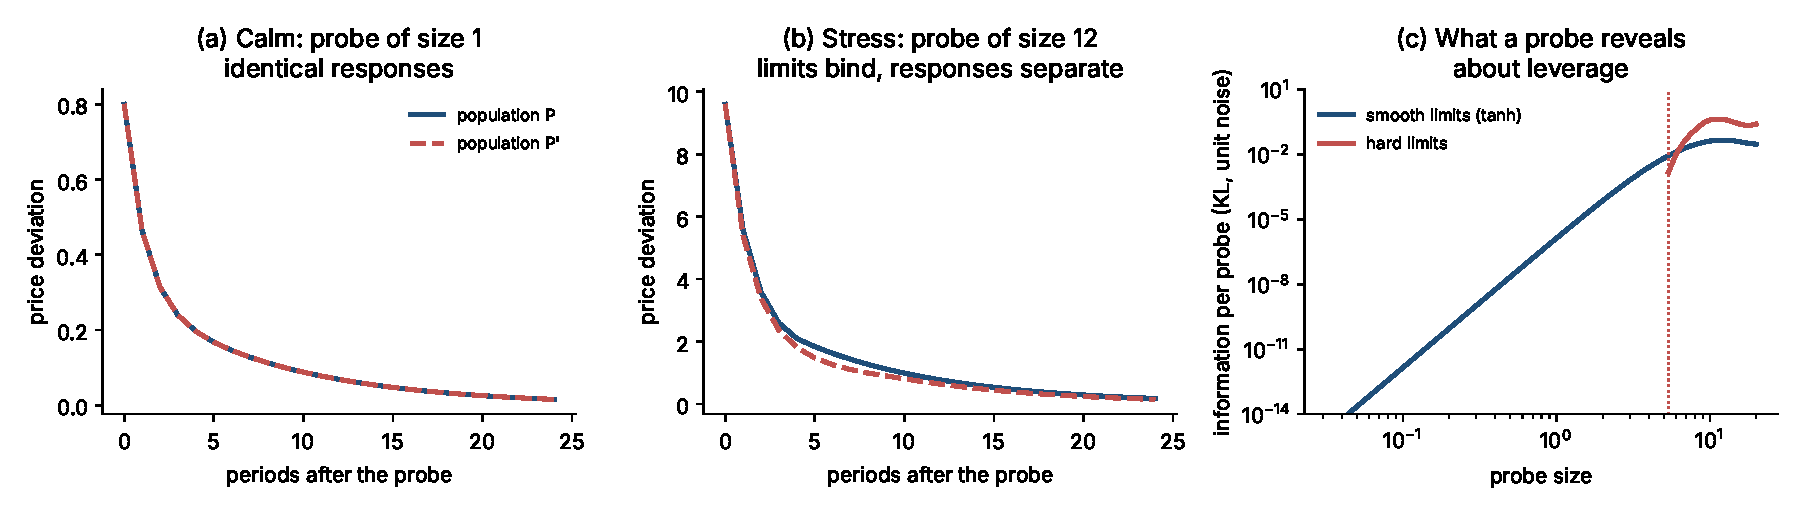
\includegraphics[width=\textwidth]{figs_core/fig_twolayer.pdf}
\caption{The two layers. Populations $P=\{(c,\ell)=(1,0.1)\}$ and $P'=\{(0.25,0.2),(1,0.05)\}$ at memory $0.7$ have the same kernel ($a=0.5$, $\kappa=0.8$). (a)~Under hard limits, a calm probe gives identical responses. (b)~A stress probe pushes the most levered trader to its limit and the responses separate. (c)~Information per probe about the difference (Kullback--Leibler divergence over 30 taps, unit noise): under smooth limits it grows like the sixth power of the probe size (fitted slope $6.00$); under hard limits it is exactly zero below the size at which the first trader reaches its limit ($5.38$, dotted).}\label{fig:twolayer}
\end{figure}

\begin{proposition}[Smooth saturation: information grows like the sixth power of the probe]\label{prop:smooth}
Let $\psi=\tanh$. In the probing experiment of Section~\ref{sec:model}, with reset state, no process noise, a single pulse of size $A$ and taps observed with independent $N(0,\sigma^2)$ noise, compare two populations $P$ and $P'$ with the same kernel and with $\rho_P=a+\kappa\sum_ic_i|\ell_i|/(1-r_i)<1$, and likewise $\rho_{P'}<1$. Let $\hat S=\max(\rho_P,\rho_{P'})$, $\Lambda_P=\tfrac13\sum_ic_i|\ell_i|^3/(1-r_i)^3$, and $\Delta M_3=\sum_ic_i\ell_i^3-\sum_jc'_j\ell_j'^{\,3}$.
\begin{enumerate}[label=(\roman*),itemsep=1pt]
\item The two price responses satisfy $\|x^P-x^{P'}\|_2\le C_D|A|^3$ with $C_D=\kappa^4(\Lambda_P+\Lambda_{P'})/(1-\hat S)^2$. Hence $N$ experiments that tell $P$ from $P'$ with both errors at most $\alpha<1/2$ need
\[
 N\ge\frac{4\sigma^2(1-2\alpha)^2}{C_D^2\,A^6}.
\]
\item The first tap after the pulse differs by $x_1^P-x_1^{P'}=-\tfrac13\kappa^4\Delta M_3A^3+O(A^5)$. If $\Delta M_3\ne0$, then for all small enough $|A|$ the averaged first tap tells $P$ from $P'$ with error at most $\alpha$ once $N\ge\bigl(12\,\sigma\,\Phi^{-1}(1-\alpha)\bigr)^2/(\kappa^8\Delta M_3^2A^6)$. So the order $A^{-6}$ is attained. The cubic coefficient of the first tap identifies $\sum_ic_i\ell_i^3$, the third leverage moment of $\nu$.
\end{enumerate}
\end{proposition}


\paragraph{In words.} Smooth saturation lets a prober learn about leverage, but slowly. Each doubling of the probe buys $64$ times the information, and the large probes that make learning cheap are the ones that push the market toward the limits being measured. Hard limits are starker: no information at all until some trader is pushed to its limit. In the example above, the first-tap gap divided by $A^3$ is $1.5359\times10^{-4}$ at $A=0.05$, against $-\tfrac13\kappa^4\Delta M_3=1.5360\times10^{-4}$.


\subsection{What stress reveals}

Theorem~\ref{thm:stress} says what calm data cannot show. The next result says what stress does show: everything that matters. Write
\[
 \tilde\mu=\sum_ic_i\,\mathrm{sgn}(\ell_i)\,\delta_{(r_i,|\ell_i|)}
\]
for the signed capacity at each memory and each leverage level. A trend follower and a contrarian with the same memory and the same leverage magnitude offset exactly, since $c\,\psi(-\ell m)=-c\,\psi(\ell m)$ for odd $\psi$.

The result holds for any shape with one property. An odd shape $\psi$ has \emph{independent dilations} if rescaled copies of it at distinct scales are linearly independent: for any distinct $s_1,\ldots,s_n>0$ and any weights $w_1,\ldots,w_n$, $\sum_kw_k\psi(s_ku)=0$ for every $u$ implies $w_1=\cdots=w_n=0$.

\begin{theorem}[Stress identifies the leverage distribution]\label{thm:satident}
Let $\psi$ be odd with independent dilations, and let every trader have $r_i\ge0$ and $\ell_i\ne0$. In the probing experiment of Section~\ref{sec:model}, with reset state and exactly observed responses, two populations give identical price responses to every probe sequence if and only if $\tilde\mu_P=\tilde\mu_{P'}$. Probe responses therefore identify, within each memory class, the net capacity at every leverage level. The kernel $k_m=\int\lambda r^m\,\tilde\mu(dr,d\lambda)$ is one linear functional of this measure.

The property holds or fails as follows.
\begin{enumerate}[label=(\roman*),itemsep=1pt]
\item The hard limit has independent dilations. For it the result needs probes of all sizes: probes that keep every memory state inside every band identify only the kernel (Theorem~\ref{thm:stress}(iv)).
\item $\tanh$ has independent dilations. Moreover, identical responses to all probes in an arbitrarily small neighbourhood of zero already imply $\tilde\mu_P=\tilde\mu_{P'}$.
\item A cubic shape $\psi(u)=u-\gamma u^3$ does not: the scales $1,2,3$ with weights $5,-4,1$ give $\sum_kw_k\psi(s_ku)=0$ for every $u$. For such a shape, probes identify only the first and third leverage moments within each memory.
\end{enumerate}
\end{theorem}

\paragraph{Machine check.} The general statement of Theorem~\ref{thm:satident} is machine-checked for any number of traders (\texttt{p1\_thm\_stress\_identification} in \nolinkurl{Paper1StressIdentificationGeneral.lean}). So are the first sentence of part~(i) (\texttt{p1\_clip\_indep\_dilations}), the first sentence of part~(ii) (\texttt{p1\_tanh\_indep\_dilations}) and the counterexample in part~(iii) (\texttt{p1\_cubic\_not\_indep\_dilations}). The theorem for the two shapes, with no hypothesis left on $\psi$, is \nolinkurl{p1_thm_stress_identification_hard_limit} and \nolinkurl{p1_thm_stress_identification_tanh}. Two things are proved on paper only: the small-probe statement in part~(ii), and the last sentence of part~(iii). In the formal statement, ``identical responses'' reads: every pair of a probe and a price path of the first market is such a pair of the second.

The proof (Supplement~\ref{app:saturating}) uses three facts. First, probes can steer the price along any path, so identical responses mean identical maps from past prices to flow. Second, two dates of prices turn that map into a sum of scaled copies of $\psi$, one per memory--leverage pair, with distinct scales for a suitable direction. Third, independent dilations separate the copies. For the hard limit, each copy adds a kink where its pair saturates, and the copy with the largest scale has the first kink. For $\tanh$, each copy approaches its limit at its own exponential rate, and the copy with the smallest scale has the slowest tail. The kink argument is constructive. In the example of Figure~\ref{fig:twolayer}, read along one direction, the flow map has kinks at $3.702$ and $14.813$, and their slope jumps return net capacities $0.24989$ and $0.99988$, against true values $0.25$ and $1$. Locating the second group needs a memory state of almost $15$, about four times the stress level at which the first trader saturates. Knowing the kernel and the first group fixes only the second group's total $c\ell$, not its leverage.

\paragraph{Relation to network identifiability.} The third step is not new mathematics. For two fixed price dates, the flow map is a network with one hidden layer and no bias terms: the activation is $\psi$, the input weights are the scales and the output weights are the capacities. For $\tanh$, \citet{sussmann1992} proved that such a network is determined by its input--output map up to permutations and sign flips of the hidden units; see also \citet{albertini1993}, \citet{fefferman1994} and \citet{vlacic2019}. The sign flip is the reason only the signed measure $\tilde\mu$ is identified. Independent dilations is the bias-free case of the independence property used in that literature. What Theorem~\ref{thm:satident} adds is the market side. Probing recovers the flow map from prices. Two price dates give distinct memory--leverage pairs distinct scales. And the identified object, the signed capacity measure, is exactly what prices depend on (Theorem~\ref{thm:satsuff}).

Theorem~\ref{thm:satident} turns Section~\ref{sec:saturating} into a two-layer theory. Prices in calm markets identify the kernel. Prices under stress identify the full signed measure $\tilde\mu$, which by Theorem~\ref{thm:satsuff} is all that any price-based outcome depends on. Under hard limits, no information beyond the kernel arrives until the first group saturates. Under smooth limits, the order-$n$ term of the response scales with the probe size to the power $2n+1$. We expect its information to scale with the power $2(2n+1)$, but only the case $n=1$ is proved (Proposition~\ref{prop:smooth}).

\subsection{Deleveraging traders and dealers who anticipate}

\begin{proposition}[Deleveraging traders]\label{prop:delever}
Let each trader follow any causal rule, for example deleveraging gradually, liquidating, or switching strategy after a loss, provided it trades linearly, $w_im_{i,t}$, as long as its state has stayed inside its band on every date up to $t$. Then Theorem~\ref{thm:stress} holds verbatim for two such populations with the same kernel. Up to the first date at which some trader leaves its band, the paths coincide and equal the linear market's path, and parts (ii)--(iv) follow.
\end{proposition}

The proof of the pathwise part is the induction of Theorem~\ref{thm:stress}(i). It is machine-checked for arbitrary causal rules outside the bands (\texttt{p1\_delever\_stress\_invariance}). Deleveraging that starts before a hard limit only moves the band edge inward. Calm data remain silent until the first trader starts to cut its position.

\paragraph{After the first breach: an open question.} What happens after a breach is not covered by these results. A natural conjecture is a threshold. If traders who breach their limits liquidate, their sales move the price, and the price move pushes other traders' states toward their own limits. One expects a cascade when the liquidation triggered per unit of price move, summed over the traders close to their limits, exceeds the market's capacity to absorb it, and no cascade otherwise. We have no proof of such a threshold and do not state one.

\begin{proposition}[Who sets prices matters]\label{prop:dealers}
\begin{enumerate}[label=(\roman*),itemsep=1pt]
\item Theorems~\ref{thm:stress} and~\ref{thm:satident} and Proposition~\ref{prop:delever} hold for any causal dealer rule that is the same in the two markets. This covers every rule that depends on the population only through its kernel, for example a dealer who knows only the kernel, or one who prices current flow.
\item A dealer who knows the population and quotes on the expected next-period feedback flow uses more than the kernel. Suppose the next memory states are Gaussian, $m^+_g\sim N(\bar m_g,s_g^2)$, with every trader inside its band in expectation, $|\ell_g\bar m_g|<1$, and hard limits. Then the expected next-period flows under two populations with the same kernel differ by at most
\[
 \sum_{g\in P\cup P'}c_g\sqrt{2/\pi}\;\sigma_g\,e^{-\delta_g^2/(2\sigma_g^2)},\qquad \sigma_g=|\ell_g|s_g,\quad\delta_g=1-|\ell_g\bar m_g|.
\]
\end{enumerate}
\end{proposition}

The proof is in Supplement~\ref{app:saturating}.

\paragraph{In words.} An informed, forward-looking dealer leaks some leverage information into calm prices, because its quote prices the chance of a breach next period. The leak is of the order of the probability of a breach, so it is exponentially small in calm markets. In the example, with expected state $2$ and standard deviation $1$, the two expected flows differ by $1.9\times10^{-5}$, within the bound $4.4\times10^{-4}$. With standard deviation $2$ they differ by $2.9\times10^{-3}$. A full equilibrium with forward-looking dealers and saturating traders is not solved here. This proposition prices only the anticipation channel.

\paragraph{What the supervisor can and cannot learn.} The two results split the population into a part prices reveal in calm markets, the kernel, and a part they reveal only under stress: the distribution of leverage within each memory, weighted by capacity. The second part decides how the market behaves when traders hit their limits, through the total capacity and through how many traders are near their limits. Calm-market price data are therefore the wrong instrument for it, however long the record and however sophisticated the estimator. The options are stress probes, whose cost and risk Proposition~\ref{prop:smooth} prices, actual stress episodes, or disclosure of capacities: position limits, margins and risk budgets. This is a different disclosure from the class-tagged flow of Section~\ref{sec:supervision}. Tagged flow reveals each group's memory and weight. Capacity disclosure reveals how far each group is from its limit.

\paragraph{What is open.} Three questions remain open. The first is rates for the higher orders of Theorem~\ref{thm:satident}: Proposition~\ref{prop:smooth} gives the first nonlinear moment, and the general order is not proved. The second is a full equilibrium with forward-looking dealers and saturating or deleveraging traders, including what happens after the first breach, in a fire sale. The third is learning agents whose rules change continuously, not only at a band edge. Related ideas appear in the literature on funding constraints and liquidity spirals \citep{brunnermeier2009} and in evidence that crowding predicts tail risk \citep{barroso2022}. The identification of sums of nonlinear branches is a known problem in system identification \citep{dreesen2017}. What is new here is the sufficient measure inside a strategic market, the exact absence of calm-market information about it, and the reduction of its recovery under stress to a known uniqueness problem.

\section{Scope and limits}\label{sec:scope}

\paragraph{Linearity.} Sufficiency (Theorem~\ref{thm:eqinv}, Proposition~\ref{prop:anylinear}) needs aggregate feedback flow to be a linear function of past public signals, plus independent idiosyncratic shocks if there are any. With group-specific Gaussian demand shocks, a second aggregate enters, the spectral density of the aggregate shock process, and the equivalence class shrinks accordingly (Supplement~\ref{app:eqinv}). The passive results of Section~\ref{sec:cost} are stated for Gaussian innovations. With non-Gaussian innovations, higher-order moments of prices could carry further information; we do not analyse that case. Saturating rules are treated in Section~\ref{sec:saturating}. Other nonlinear rules, and traders who change their rules as they learn, are outside the theorems. The full working paper reports simulations of stylized nonlinear rules and of online learners trained in the closed loop. In those simulations, the costs of Section~\ref{sec:cost} hold when the competing populations' feedback weights match. Populations whose learned weights differ are told apart by those weights instead. Hard thresholds hide groups from small probes altogether. These are simulations, not theorems.

\paragraph{Exponential memory.} The identification and cost results need memory to be a finite mixture of exponentials. For general completely monotone memory, the full working paper proves that the minimax accuracy for the memory distribution is of exact order $1/\log(N/\sigma^2)$. Halving the error then squares the data needed, instead of multiplying it by a constant.

\paragraph{The observer.} The lower bounds hold for an observer who knows $(a,\kappa)$ and the noise law, so they hold a fortiori without that knowledge. The upper bounds assume reset experiments or a known initial state. Strategic responses to being observed are modelled only in Proposition~\ref{prop:hiding}, and there for one group. Everywhere else the groups do not change their rules when probed.

\paragraph{Evidence.} The full working paper reports pre-specified tests on two sets of trader-class reports: the CFTC's weekly Commitments of Traders in twenty futures markets and Binance's class ratios in 30 perpetual markets. Of 23 recorded outcomes, 11 pass. The class reports constrain the persistence of class positions far more tightly than prices do. They do not identify learning memory, because that persistence can also reflect turnover, reporting aggregation or inventory retention. A pre-registered out-of-sample test of the feedback premise on Taiwan's tagged exchange flows (spec P1T, holdout 2019--2023; the full working paper reports every diagnostic) gives the following. $D=0.0426$ $[0.0206, 0.0643]$, $p=0.000$, meets the registered supportive criterion. The pre-specified reverse-causality check gives $D=-0.0065$ $[-0.0316, 0.0165]$, which does not meet it. The registered verdict is `supportive'. Read with its pre-specified diagnostic, the test does not provide evidence of feedback beyond prices revealing past flow. We do not claim that tagged flow in Taiwan responds to price deviations. The registered test is supportive, but its pre-specified diagnostic attributes the gain to reverse causality.

A second test, of the two-layer prediction of Section~\ref{sec:saturating}, is registered on Binance perpetual futures (spec P7S, amendment A1). Its primary sample is retrospective (July 2024 to October 2026), specified in November 2026 after the sample period, and a prospective window from November 2026 serves as a replication. The primary test was run once on 11 November 2026. A pre-specified test on Binance perpetual futures was inconclusive (calm difference $-0.002$, 90\% interval $[-0.007, 0.004]$; difference-in-differences $0.041$, $p=0.553$). It neither supports nor contradicts the prediction of Section~\ref{sec:saturating}. The prospective replication had not been run when this version was written.

\paragraph{Open problems.} Four questions remain open: a long-lived strategic insider who times her trades against the groups' memory; rates for the higher orders of the identification of saturating traders, and a full equilibrium with forward-looking dealers and deleveraging traders after a breach; sufficiency for learning agents whose rules change; and a supervisory loss function estimated from real interventions, which would turn the information costs here into a value of disclosure.

\section{Conclusion}\label{sec:conclusion}

In a linear market with feedback traders, prices summarize the trader population in one object, the feedback kernel. The kernel is sufficient for every outcome that price-based trading determines, for any insider and any causal dealer rule. It is all that prices identify, and with inventory-averse dealers both statements hold in equilibrium with unchanged memories. Information beyond the kernel, who the groups are and how much each trades, is worth nothing to anyone trading on public information. It is worth something to a supervisor whose action is aimed at a particular group. Learning it from prices costs of order $(\Delta\eta)^{-(4K-2)}$ experiments or observations, executed quantity of order $\delta^{-2}$ and capital of order $\delta^{-4}$. Class-tagged flow removes that cost. With position limits, a second layer appears: how close traders are to their limits, which calm-market prices do not reveal at all under hard limits, and which disclosure of capacities or stress alone can show.

The practical reading is a division of supervisory labour. Market-wide measures, such as limits on aggregate feedback intensity or confidence sets for the price response, can be built from public data, because they depend on the kernel alone. Targeted measures cannot be built from public data at reasonable cost when the groups' memories are close. For targeted measures, verified class-level records are the efficient source of information, not more price data or more sophisticated estimation.

\subsection*{Declarations}

\paragraph{Funding.} This research received no external funding.

\paragraph{Competing interests.} The authors declare no competing interests.

\paragraph{Author contributions.} Pratik Niroula: conceptualization, methodology, software, formal analysis, writing (original draft). Proposed review responsibilities for confirmation: Prashant Niroula and Sujan Khatiwada, proof review, validation and manuscript review. Independent human proof review and final approval by each author remain to be recorded; this draft does not attest that they have occurred.

\paragraph{Data availability.} This version analyses no new market data. It reports results of tests documented in the full working paper. The data used there are public and are listed in its data statement.

\paragraph{Code availability.} All code, pre-specified test specifications, result files and test-unlock counters are public at \url{https://github.com/Pratikn03/Fianince}. The repository's README lists the scripts in run order, and the full working paper's reproducibility appendix maps every number to the file that produces it.

\paragraph{Ethics approval.} Not applicable. The study uses only public market data and involves no human participants or personal data.

\paragraph{Use of AI tools.} Claude (Anthropic) assisted with data analysis, analysis code, derivations, Lean proofs, numerical results and text. Gemini (Google) assisted with planning and internal draft critique. ChatGPT/Codex (OpenAI) assisted with planning, literature discovery, mathematical development, code and Lean proof drafting, executable and kernel checks, result interpretation and manuscript revisions. This assistance was material. The reported kernel checks and computational runs support their explicitly stated results; they do not certify independent human review, novelty or full-manuscript correctness. AI tools are not authors. The human authors remain responsible for verifying all content, citations, analyses and conclusions and for the final scholarly contribution before submission.
\begin{thebibliography}{99}\setlength{\itemsep}{2pt}\small
\bibitem[Albertini and Sontag(1993)]{albertini1993} Albertini, F., and E.~D. Sontag (1993). For neural networks, function determines form. \emph{Neural Networks} 6, 975--990.
\bibitem[Auclert et~al.(2024)]{auclert2024} Auclert, A., M. Rognlie, and L. Straub (2024). The intertemporal Keynesian cross. \emph{Journal of Political Economy} 132, 4068--4121.
\bibitem[Barberis et~al.(2015)]{barberis2015} Barberis, N., R. Greenwood, L. Jin, and A. Shleifer (2015). X-CAPM: An extrapolative capital asset pricing model. \emph{Journal of Financial Economics} 115, 1--24.
\bibitem[Barberis et~al.(2018)]{barberis2018} Barberis, N., R. Greenwood, L. Jin, and A. Shleifer (2018). Extrapolation and bubbles. \emph{Journal of Financial Economics} 129, 203--227.
\bibitem[Barroso et~al.(2022)]{barroso2022} Barroso, P., R.~M. Edelen, and P. Karehnke (2022). Crowding and tail risk in momentum returns. \emph{Journal of Financial and Quantitative Analysis} 57, 1313--1342.
\bibitem[Batenkov et~al.(2021)]{batenkov2021} Batenkov, D., G. Goldman, and Y. Yomdin (2021). Super-resolution of near-colliding point sources. \emph{Information and Inference} 10, 515--572.
\bibitem[Brock and Hommes(1998)]{brock1998} Brock, W.~A., and C.~H. Hommes (1998). Heterogeneous beliefs and routes to chaos in a simple asset pricing model. \emph{Journal of Economic Dynamics and Control} 22, 1235--1274.
\bibitem[Brunnermeier and Pedersen(2009)]{brunnermeier2009} Brunnermeier, M. K., and L. H. Pedersen (2009). Market liquidity and funding liquidity. \emph{Review of Financial Studies} 22, 2201--2238.
\bibitem[Cagan(1956)]{cagan1956} Cagan, P. (1956). The monetary dynamics of hyperinflation. In M. Friedman (Ed.), \emph{Studies in the Quantity Theory of Money}, 25--117. University of Chicago Press.
\bibitem[Celov et~al.(2008)]{celov2008} Celov, D., R. Leipus, and A. Philippe (2008). Asymptotic normality of the mixture density estimator in a disaggregation scheme. arXiv preprint arXiv:0802.0817.
\bibitem[De Long et~al.(1990)]{delong1990} De Long, J. B., A. Shleifer, L. H. Summers, and R. J. Waldmann (1990). Positive feedback investment strategies and destabilizing rational speculation. \emph{Journal of Finance} 45, 379--395.
\bibitem[Dreesen et~al.(2017)]{dreesen2017} Dreesen, P., D.~T. Westwick, J. Schoukens, and M. Ishteva (2017). Modeling parallel Wiener--Hammerstein systems using tensor decomposition of Volterra kernels. arXiv preprint arXiv:1609.08063.
\bibitem[Fefferman(1994)]{fefferman1994} Fefferman, C. (1994). Reconstructing a neural net from its output. \emph{Revista Matem\'atica Iberoamericana} 10, 507--555.
\bibitem[Forni and Lippi(1997)]{forni1997} Forni, M., and M. Lippi (1997). \emph{Aggregation and the Microfoundations of Dynamic Macroeconomics}. Oxford University Press.
\bibitem[Granger(1980)]{granger1980} Granger, C. W. J. (1980). Long memory relationships and the aggregation of dynamic models. \emph{Journal of Econometrics} 14, 227--238.
\bibitem[Grossman and Miller(1988)]{grossman1988} Grossman, S. J., and M. H. Miller (1988). Liquidity and market structure. \emph{Journal of Finance} 43, 617--633.
\bibitem[Heinrich and Kahn(2018)]{heinrich2018} Heinrich, P., and J. Kahn (2018). Strong identifiability and optimal minimax rates for finite mixture estimation. \emph{Annals of Statistics} 46, 2844--2870.
\bibitem[Ho and Stoll(1981)]{hostoll1981} Ho, T., and H. R. Stoll (1981). Optimal dealer pricing under transactions and return uncertainty. \emph{Journal of Financial Economics} 9, 47--73.
\bibitem[Katz et~al.(2023)]{katz2023} Katz, R., N. Diab, and D. Batenkov (2023). On the accuracy of Prony's method for recovery of exponential sums with closely spaced exponents. arXiv preprint arXiv:2302.05883.
\bibitem[Koyck(1954)]{koyck1954} Koyck, L.~M. (1954). \emph{Distributed Lags and Investment Analysis}. North-Holland.
\bibitem[Kyle(1985)]{kyle1985} Kyle, A. S. (1985). Continuous auctions and insider trading. \emph{Econometrica} 53, 1315--1335.
\bibitem[Lecl\`ere and Rosenbaum(2026)]{leclere2026} Lecl\`ere, J., and M. Rosenbaum (2026). Mean-field equilibrium of heterogeneous agents under market impact. arXiv preprint arXiv:2609.03115.
\bibitem[Moitra(2015)]{moitra2015} Moitra, A. (2015). Super-resolution, extremal functions and the condition number of Vandermonde matrices. In \emph{Proceedings of the 47th Annual ACM Symposium on Theory of Computing (STOC)}, 821--830.
\bibitem[Muth(1960)]{muth1960} Muth, J.~F. (1960). Optimal properties of exponentially weighted forecasts. \emph{Journal of the American Statistical Association} 55, 299--306.
\bibitem[Nerlove(1958)]{nerlove1958} Nerlove, M. (1958). Adaptive expectations and cobweb phenomena. \emph{Quarterly Journal of Economics} 72, 227--240.
\bibitem[Niroula et~al.(2026)]{niroula2026b} Niroula, P., S. Alkhushayni, Y. Chen, M. Bhavsar, and P. Niroula (2026). From human markets to machine markets: Transient amplification, an exact depth condition, and a maximal pre-trade guard. Working paper, Minnesota State University, Mankato.
\bibitem[Pesaran and Chudik(2014)]{pesaran2014} Pesaran, M.~H., and A. Chudik (2014). Aggregation in large dynamic panels. \emph{Journal of Econometrics} 178, 273--285.
\bibitem[Sargent(1976)]{sargent1976} Sargent, T.~J. (1976). The observational equivalence of natural and unnatural rate theories of macroeconomics. \emph{Journal of Political Economy} 84, 631--640.
\bibitem[Sussmann(1992)]{sussmann1992} Sussmann, H.~J. (1992). Uniqueness of the weights for minimal feedforward nets with a given input-output map. \emph{Neural Networks} 5, 589--593.
\bibitem[Tsybakov(2009)]{tsybakov2009} Tsybakov, A. B. (2009). \emph{Introduction to Nonparametric Estimation}. Springer.
\bibitem[Vla\v{c}i\'c and B\"olcskei(2019)]{vlacic2019} Vla\v{c}i\'c, V., and H. B\"olcskei (2019). Neural network identifiability for a family of sigmoidal nonlinearities. arXiv preprint arXiv:1906.06994.
\bibitem[Wu and Yang(2020)]{wu2020} Wu, Y., and P. Yang (2020). Optimal estimation of Gaussian mixtures via denoised method of moments. \emph{Annals of Statistics} 48, 1981--2007.
\bibitem[Zaffaroni(2004)]{zaffaroni2004} Zaffaroni, P. (2004). Contemporaneous aggregation of linear dynamic models in large economies. \emph{Journal of Econometrics} 120, 75--102.
\end{thebibliography}
\appendix
\clearpage
\singlespacing\small\sloppy
\renewcommand{\topfraction}{0.9}\renewcommand{\bottomfraction}{0.8}\renewcommand{\textfraction}{0.07}\renewcommand{\floatpagefraction}{0.75}
\setcounter{page}{1}\renewcommand{\thepage}{S-\arabic{page}}\renewcommand{\thesection}{S\arabic{section}}\setcounter{table}{0}\renewcommand{\thetable}{S\arabic{table}}\setcounter{figure}{0}\renewcommand{\thefigure}{S\arabic{figure}}
\begin{center}{\Large Online Supplement}\\[4pt]{\large A Sufficient Statistic for Algorithmic Feedback}\\[2pt]{\normalsize Niroula, Niroula and Khatiwada, core version, 11 November 2026}\end{center}

\noindent The supplement contains the proofs of the results stated in the main text (Section~\ref{app:proofs}), the further equilibrium results with their proofs (Section~\ref{app:eqinv}), execution cost and capital (Section~\ref{app:capital}), the two-group case used by Theorem~\ref{prop:passive}(ii) (Section~\ref{app:twocohort}), the supervisory decision in detail, with the targeted halt for every $K$ (Section~\ref{app:decisionfull}), the proofs for saturating traders (Section~\ref{app:saturating}), machine checks in detail (Section~\ref{app:mc}), the machine-checked declarations (Section~\ref{app:verification}) and the notation (Section~\ref{app:notation}). Proofs of results that also appear in the full working paper of 5 November 2026 are taken from it. Two things are changed in them: cross-references to material not included here, and the word for a trader group, which the full paper calls a ``co\-hort''. The proofs for Section~\ref{sec:saturating} and for Section~\ref{app:everyK} are new.

\section{Proofs of the main results}\label{app:proofs}

\paragraph{A lemma used in the proofs.}
\begin{lemma}[Positive price-response geometry]\label{lem:cm}
In the positive, stable economy the impulse response is a nonnegative mixture of decaying exponentials,
\[
h_j=\sum_\ell \omega_\ell\lambda_\ell^j,\qquad \omega_\ell\ge0,\quad \sum_\ell\omega_\ell=\kappa,\quad 0\le\lambda_\ell<1 .
\]
It is completely monotone and nonincreasing; its peak is the direct impact $\kappa$, even though $J$ is non-normal. In price/memory coordinates the price-only gain is $\sup_t\|e_x^\top J^t\|_2=1$.
\end{lemma}

\paragraph{Lemma~\ref{lem:cm}.} Omit zero-weight groups. For $a>0$ put $b_i=\kappa q_i$ and
\[
T={\rm diag}\bigl(\sqrt a,\sqrt{b_1/\eta_1},\ldots\bigr),\qquad u=\bigl(\sqrt a,\sqrt{b_1\eta_1},\ldots\bigr)^\top .
\]
The price-first transition becomes the symmetric matrix $J'=TJT^{-1}={\rm diag}(0,r_1,\ldots)+uu^\top$, the input transforms to $\kappa u$ and $J'e_x=\sqrt a\,u$, so $h_j=(\kappa/a)e_x^\top(J')^{j+1}e_x$. The spectral decomposition of $J'$ gives nonnegative weights summing to $h_0=\kappa$, and Schur stability puts the eigenvalues in $[0,1)$. The case $a=0$ follows by continuity. A nonnegative mixture of decaying geometric sequences is completely monotone. Since $J$ is nonnegative with row sums at most one, every price row of $J^t$ has $\ell_1$, hence $\ell_2$, norm at most one, attained at $t=0$.


\paragraph{Lemma~\ref{lem:micro}.} (i) For $v_{t+1}=v_t+\zeta_{t+1}$ and $r_t=v_t+\nu_t$, the steady-state prior variance $P$ solves $P=P\sigma_\nu^2/(P+\sigma_\nu^2)+\sigma_\zeta^2$, i.e.\ $P^2-\sigma_\zeta^2P-\sigma_\zeta^2\sigma_\nu^2=0$, whose positive root is $P=\bigl(\sigma_\zeta^2+\sqrt{\sigma_\zeta^4+4\sigma_\zeta^2\sigma_\nu^2}\bigr)/2$. The gain is $\eta=P/(P+\sigma_\nu^2)\in(0,1)$, which simplifies to \eqref{eq:kgain}, and the update $\hat v_{t+1}=\hat v_t+\eta(r_t-\hat v_t)$ has the stated form. (ii) $\nabla_\theta\tfrac12H(x_t-\theta)^2=-H(x_t-\theta)$, so $\theta_{t+1}=(1-\gamma)\theta_t+\alpha H(x_t-\theta_t)=(1-\eta)\theta_t+\eta qx_t$ with $\eta=\gamma+\alpha H$ and $q=\alpha H/\eta$.


\paragraph{Theorem~\ref{thm:merged}.} With zero initial states, $y_{i,t}=\sum_{s\le t}\eta_ir_i^{t-s}x_s$, so $\sum_iq_iy_{i,t}=\sum_{s\le t}k_{t-s}x_s$ and every response is determined by $(a,\kappa,k)$, hence by $M$. Conversely, equal responses for all probes imply equal $H$, hence equal $G$, and partial fractions of $G$ identify the distinct poles with nonzero residues $w_i$, i.e.\ $M$. After cancellation, $H=\kappa zD(z)/[(z-a)D(z)-\kappa N(z)]$ with $D=\prod(z-r_i)$ and $N(z)=\sum_iw_iz\prod_{j\ne i}(z-r_j)$, as in \eqref{eq:H}; at a retained $r_i$ the denominator equals $-\kappa N(r_i)=-\kappa w_ir_i\prod_{j\ne i}(r_i-r_j)\neq0$ (memory rates are positive because $\eta_i<1$), so no root of $D$ cancels. The numerator $\kappa zD(z)$ has no roots other than $0$ and the $r_i$, so these are the only possible cancellations. The remaining numerator factor $z$ cancels if and only if the denominator vanishes at $0$; since $N(0)=0$ the denominator there equals $-aD(0)$, which is nonzero for $a>0$ and zero for $a=0$. Hence the McMillan degree, which is the dimension of a minimal realization, is $1+|{\rm supp}(M)\cap(0,1)|$ for $a'\neq0$ and $|{\rm supp}(M)\cap(0,1)|$ for $a'=0$ (an atom at rate $0$, a group with $\eta=1$, contributes the constant $M(\{0\})$ to $G$ and no pole, so it shifts $a$ to $a'=a+\kappa M(\{0\})$ and the argument above applies with $a'$) (numerically, the rank of the Hankel matrix of $(h_j)_{j\ge1}$ is $K+1$ and $K$ respectively for $K=1,2,3$). For (ii), direct algebra gives
\[
G_\delta(z)-G_0(z)=-\frac{qz(z-1)\delta^2}{(z-1+\bar\eta)\bigl((z-1+\bar\eta)^2-\delta^2\bigr)} .
\]
The denominator is the product of the three linear factors $z-r$ with $r\in\{1-\bar\eta,\,1-\bar\eta\pm\delta\}$, all in $[\epsilon,1-\epsilon]$ by assumption; on $|z|=1$ each satisfies $|z-r|\ge1-r\ge\epsilon$, so $|G_\delta-G_0|\le2q\delta^2/\epsilon^3$ there. Uniform stability gives $M_H=\sup|H_\theta|<\infty$, and the identity $H_\delta-H_0=z^{-1}H_\delta H_0(G_\delta-G_0)$, whose factor $z^{-1}$ has modulus one on the circle, gives an $\ell_2$ gain at most $C_{\mathcal F}\delta^2$. The mean difference of a power-constrained probe has squared norm at most $C_{\mathcal F}^2\delta^4PT$; the equal-noise KL is at most $C_{\mathcal F}^2\delta^4PT/(2\sigma_\nu^2)$, and Pinsker's inequality with total variation at least $1-2\alpha$ gives \eqref{eq:Tpower}.


\paragraph{Theorem~\ref{thm:kcohort}.} Let $(s^A,\omega^A)$ and $(s^B,\omega^B)$ be the $K$-point Gauss and Gauss--Radau rules for the uniform weight on $[-1,1]$, normalized to unit mass. Both are positive and exact for polynomials of degree $2K-2$, and their moments of degree $2K-1$ differ by $g_K\neq0$. To see that $g_K\ne0$, let the Radau nodes be $-1,s_2,\ldots,s_K$ and put $P(s)=(s+1)\prod_{j\ge2}(s-s_j)^2$. This is monic of degree $2K-1$ and vanishes at every Radau node, so the Radau rule gives it $0$. Gauss is exact to degree $2K-1$, so it gives $\int P\,d\mu>0$, since $P\ge0$ on $[-1,1]$ and vanishes only at the nodes. The two rules agree on every lower-degree term, so they differ on $s^{2K-1}$. Put $r=r_c+\Delta\eta\,s$ and weights $W\omega$, and let $\mu^X_j=W\sum_i\omega^X_i(s^X_i)^j$ for $X\in\{A,B\}$. Then $|\mu^X_j|\le W$, and $\mu^A_j=\mu^B_j$ for $j\le2K-2$.

\emph{Kernel gap.} By the binomial theorem, $k^X_m=\sum_j\binom mj r_c^{m-j}(\Delta\eta)^j\mu^X_j$. So, with $n=2K-1$, $\Delta k_m=k^A_m-k^B_m=\sum_{j\ge n}\binom mj r_c^{m-j}(\Delta\eta)^j(\mu^A_j-\mu^B_j)$. Since $\binom mj\le\binom mn\binom{m-n}{j-n}$ for $j\ge n$, this gives $|\Delta k_m|\le2W\binom mn(\Delta\eta)^n(r_c+\Delta\eta)^{m-n}$. Summing with $\sum_m\binom mn x^{m-n}=(1-x)^{-(n+1)}$ gives $\|\Delta k\|_1\le2W(\Delta\eta)^{2K-1}/(1-r_c-\Delta\eta)^{2K}$ over all lags.

\emph{Response gap.} Let $\varsigma=a+\kappa W/(1-r_c-\Delta\eta)<1$, the theorem's hypothesis. Each kernel has $\|k^X\|_1\le W/(1-r_c-\Delta\eta)$. From $h_0=\kappa$ and $h_{t+1}=ah_t+\kappa\sum_jk_jh_{t-j}$, every partial sum of $|h^B|$ is at most $\kappa/(1-\varsigma)$. The difference $\Delta h=h^A-h^B$ has $\Delta h_0=0$ and $\Delta h_{t+1}=a\Delta h_t+\kappa\sum_j\bigl(k^A_j\Delta h_{t-j}+\Delta k_jh^B_{t-j}\bigr)$, so every partial sum of $|\Delta h|$ is at most $\kappa\|\Delta k\|_1\|h^B\|_1/(1-\varsigma)$. Hence, for every horizon,
\[
\|h^A-h^B\|_2\le\|h^A-h^B\|_1\le C_U(\Delta\eta)^{2K-1},\qquad C_U=\frac{2\kappa^2W}{(1-r_c-\Delta\eta)^{2K}(1-\varsigma)^2}.
\]
In the other direction, $\Delta k_j=0$ for $j<2K-1$, so by induction $\Delta h_t=0$ for $t\le2K-1$, and $\Delta h_{2K}=\kappa\,\Delta k_{2K-1}h^B_0=\kappa^2Wg_K(\Delta\eta)^{2K-1}$. When the taps $h_0,\ldots,h_{T-1}$ are observed with $T\ge2K+1$, this gives $\|h^A-h^B\|_2\ge\kappa^2W|g_K|(\Delta\eta)^{2K-1}$. With $T\le2K$ the observed responses coincide. The impossibility bound holds for every $T$, since it uses only the upper order.

\emph{Testing.} $N$ reset experiments have divergence $N\|h^A-h^B\|_2^2/(2\sigma^2)$. By Pinsker's inequality, a test whose two error probabilities are at most $\alpha$ needs divergence at least $2(1-2\alpha)^2$. So $N\ge4(1-2\alpha)^2\sigma^2(\Delta\eta)^{-(4K-2)}/C_U^2$, and the constant does not depend on $T$. For the $W_1$ version, the two merged measures are the images of the fixed normalized rules under $s\mapsto r_c+\Delta\eta\,s$ scaled to mass $W$, so their distance is $W\Delta\eta$ times the distance $2c_K>0$ between the rules, and the same two-point argument applies with the metric loss.


\paragraph{Theorem~\ref{prop:passive}.} For stationary Gaussian processes with spectral densities $f_j\propto|H_j(e^{i\omega})|^2$, the divergence rate is
\[
D=\frac1{4\pi}\int_{-\pi}^{\pi}\bigl(\varrho-1-\log\varrho\bigr)\,d\omega,\qquad \varrho=f_1/f_0=|H_1/H_0|^2 .
\] By the resolvent identity, $H_1/H_0-1=z^{-1}H_1\Delta G$ with $\Delta G=G_1-G_0$, and uniform stability bounds $|H_1|$ on the circle, so $u\equiv\varrho-1=2\,{\rm Re}(z^{-1}H_1\Delta G)+O(|\Delta G|^2)$. Write $G(z)=\sum_kw_k\phi(z,\eta_k)$, with $w_k$ the group weights (any factor of $\eta_k$ is absorbed in $\phi$), where $\phi$ is analytic in $\eta$ on a neighbourhood of $[\eta_{\min},\eta_{\max}]$ uniformly for $|z|=1$ (its pole $z=1-\eta$ stays inside the disk). Expanding $\phi$ around $\bar\eta$, $\Delta G=\sum_{j\ge0}\frac{\partial_\eta^j\phi(z,\bar\eta)}{j!}\,\Delta\tilde M_j$, where $\tilde M_j=\sum_kw_k(\eta_k-\bar\eta)^j$. For the pair, $\Delta\tilde M_0=\Delta\tilde M_1=0$ and $\Delta\tilde M_2=q\delta^2$; for the moment-matched economies, $\Delta\tilde M_j=0$ for $j\le2$ and $\Delta\tilde M_3=4\tau p_-p_+(\Delta\eta)^3$ by \eqref{eq:dM3}; for the $K$-group Gauss and Gauss--Radau economies with rates $\bar\eta+\Delta\eta\,s$ and weights $W\omega$, both rules integrate polynomials of degree $2K-2$ exactly, so $\Delta\tilde M_j=W(\Delta\eta)^j\sum_k(\omega^A_k(s^A_k)^j-\omega^B_k(s^B_k)^j)$ vanishes for $j\le2K-2$ and equals $\pm Wg_K(\Delta\eta)^{2K-1}\neq0$ at $j=2K-1$. Higher terms are smaller by a factor of the spacing: $|\Delta\tilde M_j|\le2W(\Delta\eta)^j$, and analyticity of $\phi$ in $\eta$ on a disk of radius $\varrho>0$ around $\bar\eta$, uniformly on the circle, gives $|\partial_\eta^j\phi|/j!\le C\varrho^{-j}$, so for $\Delta\eta<\varrho/2$ the tail beyond the first nonzero term is $O((\Delta\eta)^{j_0+1})$. Hence $\sup_\omega|u|=O(\delta^2)$, $O(\tau(\Delta\eta)^3)$, respectively $O((\Delta\eta)^{2K-1})$, and $u=c(\omega)\epsilon+o(\epsilon)$ with $\epsilon=\delta^2$, $\tau(\Delta\eta)^3$ or $(\Delta\eta)^{2K-1}$ and $c(\omega)$ proportional to $2\,{\rm Re}\bigl(z^{-1}H_0\,\partial^{j_0}_\eta\phi(\cdot,\bar\eta)\bigr)/j_0!$, $j_0=2$, $3$ or $2K-1$. The function $c$ does not vanish identically: $f=z^{-1}H_0\partial^j_\eta\phi$ is analytic outside the disk including at infinity, where it vanishes, and is not identically zero; an analytic function on the exterior whose real part vanishes on the circle is an imaginary constant, which here would have to be zero. For $|u|\le\frac12$, $u^2/4\le u-\log(1+u)\le u^2$, so $D\asymp\int c(\omega)^2d\omega\,\epsilon^2$, which gives (i)--(iii). The sample requirements need a finite-$T$ bound that is uniform in the separation, which we obtain directly. The first $T$ observations are $N(0,\Sigma_j)$ with $\Sigma_j$ the $T\times T$ Toeplitz matrices of the spectral densities $f_j=\sigma^2|H_j(e^{i\omega})|^2$. On the compact, uniformly stable family the transfer functions have no zeros or poles on the circle (Theorem~\ref{thm:minphase}), so $0<\underline f\le f_j\le\bar f<\infty$ with constants that do not depend on the separation. A Toeplitz matrix has eigenvalues within the range of its symbol, so $\lambda_{\min}(\Sigma_0)\ge\underline f$ and $\|\Sigma_1-\Sigma_0\|\le\sup_\omega|f_1-f_0|=\sup_\omega f_0|u|\le\bar f\sup_\omega|u|$. With $A=\Sigma_0^{-1/2}\Sigma_1\Sigma_0^{-1/2}$, whose eigenvalues lie in $[\underline f/\bar f,\bar f/\underline f]$, the inequality $\lambda-1-\log\lambda\le(\lambda-1)^2/\lambda$ gives
\[
\KL(P_1^T\|P_0^T)=\tfrac12\sum_k(\lambda_k-1-\log\lambda_k)\le\frac{\bar f}{2\underline f}\,\|A-I\|_F^2\le\frac{\bar f}{2\underline f}\,T\Bigl(\frac{\bar f}{\underline f}\Bigr)^2\sup_\omega|u|^2\le C\,T\epsilon^2,
\]
with $C$ independent of $T$ and of the separation, because $\sup_\omega|u|=O(\epsilon)$ uniformly. The Bretagnolle--Huber inequality \citep[Lemma 2.6]{tsybakov2009} then gives the stated lower bounds on $T$ for every $T$, not only asymptotically. For a fixed pair, $T^{-1}\KL(P_1^T\|P_0^T)\to D$ and Stein's lemma (one error fixed) and the Chernoff bound (both errors vanishing) give the error exponents of the likelihood-ratio test, of the same order in the separation; that statement is pointwise in the pair.


\paragraph{Theorem~\ref{thm:minphase}.} In the delay variable $\lambda=z^{-1}$, $H=\kappa\prod_i(1-r_i\lambda)/\bigl[(1-a\lambda)\prod_i(1-r_i\lambda)-\kappa\lambda\sum_iw_i\prod_{j\ne i}(1-r_j\lambda)\bigr]$, which is \eqref{eq:H} divided through by $z^{K+1}$; its nonstructural zeros are the memory rates, which do not cancel under the nondegenerate assumptions of Theorem~\ref{thm:minphase}. In the z-plane there is also the structural timing zero at zero: the numerator is proportional to $z\prod_i(z-r_i)$. Stability puts the poles inside the disk. A rational spectral density $\sigma^2|H(e^{i\omega})|^2$ has a unique minimum-phase factor up to a unimodular constant, which is $H$; Theorem~\ref{thm:merged} then gives the merged measure.


\paragraph{Proposition~\ref{prop:tagged}.} With tagged flow, $u_{i,t}=r_iu_{i,t-1}+w_ix_t$ holds exactly and involves only group $i$, so $\tilde u_{i,t}=r_i\tilde u_{i,t-1}+w_ix_t+e_{i,t}$ with the MA(1) error $e_{i,t}$. Prices are independent of the measurement noise, so $\E[Z_te_{i,t}]=0$ and, by the ergodic theorem for the stationary linear price process, the IV estimator is consistent when $\Sigma_i=\E[Z_t(\tilde u_{i,t-1},x_t)]$ is nonsingular. Since $u_{i,t-1}=w_i\sum_{s\ge0}r_i^sx_{t-1-s}$, $\E[x_{t-1}u_{i,t-1}]=w_iA_0$ and $\E[x_tu_{i,t-1}]=w_iA_1$, which gives $\Sigma_i$. The price is a nonnegative mixture of geometric responses to its innovation (Lemma~\ref{lem:cm}), so $\gamma_x(s)=\sum_\ell c_\ell\lambda_\ell^{s}$ with $c_\ell=\sigma_\xi^2\kappa^{-2}\omega_\ell\sum_m\omega_m/(1-\lambda_\ell\lambda_m)\ge0$; substituting, $\det\Sigma_i=w_i(\gamma_x(0)A_0-\gamma_x(1)A_1)=w_i\sum_{\ell,m}c_\ell c_m(1-\lambda_\ell\lambda_m)/(1-r_i\lambda_m)$, each term positive. By summation by parts, $\sum_{t=1}^TZ_te_{i,t}=\sum_{t=1}^T(Z_t-r_iZ_{t+1})\varepsilon_{i,t}+O_P(1)$. Since $(\varepsilon_{i,t})$ is i.i.d.\ with mean zero and variance $\sigma_f^2$ and independent of the whole stationary price process, the summands $m_t=(Z_t-r_iZ_{t+1})\varepsilon_{i,t}$ form a stationary ergodic martingale difference sequence with respect to $\mathcal F_t=\sigma((x_s)_{s\in\mathbb Z},\varepsilon_{i,s}:s\le t)$, with $\E[m_tm_t^\top]=\sigma_f^2[(1+r_i^2)\Gamma_0-r_i(\Gamma_1+\Gamma_1^\top)]=\Omega_i$, so the Billingsley--Ibragimov martingale central limit theorem gives \eqref{eq:ivvar}. On a uniformly stable family the modes and weights lie in a compact set with $\lambda_\ell\le\bar\lambda<1$, so with $w_i\ge w_{\min}>0$ we get $\det\Sigma_i\ge w_{\min}(1-\bar\lambda^2)\gamma_x(0)^2>0$ and $\|\Omega_i\|$ is bounded, uniformly in the spacing.


\paragraph{Theorem~\ref{prop:esprit}.}
\begin{proof}
The kernel values $k_m=\sum_iw_ir_i^m$ are the power moments of the merged measure. The closed-loop recursion $h_t=ah_{t-1}+\kappa\sum_mk_mh_{t-1-m}$ (plus $\kappa$ at $t=0$) can be solved for $k_0,\ldots,k_{2K-1}$ from $h_1,\ldots,h_{2K}$. Because $h_0=\kappa$ is a known primitive, each $k_m$ is a polynomial in $h_1,\ldots,h_{m+1}$ with coefficients depending on $(a,\kappa)$ (the only division is by $\kappa h_0=\kappa^2$), so on the bounded set of responses within sup-distance $1$ of the class this map is $L_h$-Lipschitz, with $L_h$ depending on the class but not on $\Delta\eta$. Let $E$ be the event $\max_{1\le t\le2K}|\bar h_t-h_t|\le\sigma N^{-1/2}\sqrt{2\log(4K/\beta)}$, where $\bar h_t$ averages the $N$ responses; a Gaussian tail bound and a union bound over the $2K$ estimated taps give $P(E)\ge1-\beta$. On $E$, and provided this radius is at most $1$, the estimated kernel values satisfy $\max_m|\hat k_m-k_m|\le L_h\sigma N^{-1/2}\sqrt{2\log(4K/\beta)}$. Centring at $r_c$ is a fixed triangular linear map, $\mu_m=\sum_{j\le m}\binom mj(-r_c)^{m-j}k_j$, and $\mu_m=(\Delta\eta)^m t_m$ with $t_m=\sum_iw_is_i^m$. The map $F:(s,\omega)\mapsto(t_0,\ldots,t_{2K-1})$ does not depend on $\Delta\eta$; its Jacobian is a confluent Vandermonde matrix with determinant $\prod_i\omega_i\prod_{i<j}(s_i-s_j)^4$, bounded away from zero on the compact class. On ordered, $\gamma$-separated nodes $F$ is injective, because a measure with $K$ distinct atoms is determined by its first $2K$ moments. A $C^1$ map that is injective on a compact set $Q$ and has a nonsingular Jacobian there is injective on an open neighbourhood $U$ of $Q$: otherwise there are $x_n\ne y_n$ with $F(x_n)=F(y_n)$ and distance to $Q$ tending to zero, whose limits $x,y\in Q$ satisfy $F(x)=F(y)$, so $x=y$, contradicting local injectivity at $x$. Applying the quantitative inverse function theorem uniformly on $Q$, there are $\rho_0>0$ and $L<\infty$, uniform over the class, such that $F(U)$ contains the ball of radius $\rho_0$ around every point of $F(Q)$ and the single inverse $F^{-1}:F(U)\to U$ is $L$-Lipschitz on each such ball. An error $e$ in $\mu_m$ is an error $e(\Delta\eta)^{-m}$ in $t_m$, largest at $m=2K-1$. Since $\Delta\eta<1$ and the centring map is fixed, on $E$ we get $\|\hat t-t\|_\infty\le C_1\sqrt{\log(4K/\beta)}\,\epsilon_N$ with $C_1$ equal to $\sqrt2L_h$ times the norm of the centring map; and because $\sigma N^{-1/2}\sqrt{2\log(4K/\beta)}\le\sqrt2\,\epsilon_N\sqrt{\log(4K/\beta)}$, the radius condition holds whenever $c_0\le1/\sqrt2$. When this is below $\rho_0$, $\hat t$ lies in the ball where $F^{-1}$ is $L$-Lipschitz. For an input in such a ball, $x=F^{-1}(\hat t)$ has $K$ distinct nodes and nonzero weights, so the $K\times K$ Hankel matrix of $\hat t$ is nonsingular and Prony's method returns exactly $x$: the Prony polynomial is determined uniquely by the Hankel system, and since the $K$ real nodes of $x$ reproduce $\hat t$ it equals $\prod_i(z-\hat s_i)$, so its roots are real and distinct and no complex pair can appear; Prony's method computes the algebraic inverse of the moment map up to the order of the atoms, so, listing its output in increasing order of rate (which the error bound below keeps unambiguous once $C\sqrt{\log(4K/\beta)}\,\epsilon_N<\gamma/2$), its output is $F^{-1}(\hat t)$ and the stated bound follows with $C=LC_1$ and $c_0=\min\{\min(\rho_0,\gamma/(2L))/C_1,\,1/\sqrt2\}$, which also keeps $C\sqrt{\log(4K/\beta)}\,\epsilon_N<\gamma/2$. No separate root-perturbation bound is needed: on the ball where $F^{-1}$ is $L$-Lipschitz, Prony's roots and weights are the coordinates of $F^{-1}(\hat t)$, so the conditioning of the root step is part of $L$ (for an explicit step-by-step analysis of Prony's method with clustered exponents see \citealp{katz2023}). The matching statement requires the class to contain the Gauss and Gauss--Radau pair of Theorem~\ref{thm:kcohort} (ordered nodes with separation at least the smaller of their two minimum gaps, and weights within $[\omega_{\min},\omega_{\max}]$ after scaling to total weight $W$); for any such class the orders match, with constants that depend on the class.
\end{proof}
\paragraph{Theorem~\ref{thm:discvalue}.}
\begin{proof}
$N_p\asymp\sigma^2(\Delta\eta)^{-(4K-2)}$ by Theorems~\ref{thm:kcohort} and~\ref{prop:esprit}. \emph{Upper bounds.} Average the $N$ price responses to estimate $h$ with error of order $\sigma N^{-1/2}$ per tap. Given $h$, class $i$'s mean flow is a two-parameter family $F(w_i,r_i;h)$ whose Jacobian columns $\sum_sr_i^{t-s}h_s$ and $w_i\sum_s(t-s)r_i^{t-s-1}h_s$ are linearly independent, with a Gram determinant bounded below uniformly on the class because $w_i\ge\omega_{\min}$, the rates lie in a compact subset of $(0,1)$ and $h_0=\kappa>0$; the bound does not involve the other classes or $\Delta\eta$. Least squares on class $i$'s flows with the plug-in $h$ therefore estimates $(w_i,r_i)$ with error $O_P(N^{-1/2})$, uniformly on the class, which gives the upper bounds in (i) and in (ii) for accuracy $\epsilon\Delta\eta$. For (i) there is also a finite-sample version: in the first period the tagged flow of class $i$ is $w_i\kappa$, so the mean of the $N$ first-period records gives $P(|\hat w_i-w_i|\ge\epsilon)\le\sigma_f^2/(N\kappa^2\epsilon^2)$ by Chebyshev's inequality, for every configuration (this step is machine-checked). \emph{Lower bounds.} At a configuration in the interior of the class, perturb one class's weight by $\epsilon$, or its rate by $\epsilon\Delta\eta$; for small $\epsilon$ both perturbed configurations remain in the class because the weight interval is nondegenerate and the rate set has nonempty interior. The mean differences of both the price and the flow records are of order $\epsilon$, respectively $\epsilon\Delta\eta$, so the Kullback--Leibler divergence of $N$ experiments is at most $CN\epsilon^2$, respectively $CN\epsilon^2(\Delta\eta)^2$, and Le Cam's two-point lemma gives the lower bounds.
\end{proof}

\paragraph{Unknown primitives.}
\begin{corollary}[Unknown primitives cost nothing in the rate]
\label{cor:unknown_primitives}
In the setting of Theorem~\ref{prop:esprit}, suppose in addition that every memory rate is at least $\varepsilon>0$ (that is, $r_c-\Delta\eta\ge\varepsilon$), and that the fundamental value $p^*$, the impact $\kappa\in[\underline\kappa,\overline\kappa]\subset(0,\infty)$ and the persistence $a\in[0,\bar a]\subset[0,1)$ are unknown. Put $\tilde k_0=k_0+a/\kappa$ and $\tilde k_m=k_m$ for $m\ge1$.
\begin{enumerate}[label=(\roman*)]
\item The response depends on $(a,\kappa,M)$ only through $\kappa$ and $\tilde k$: $h_0=\kappa$ and $h_{t+1}=\kappa\sum_{m=0}^{t}\tilde k_mh_{t-m}$. The persistence $a$ acts exactly like an extra group with memory rate zero and merged weight $a/\kappa$.
\item The taps $h_0,\ldots,h_{2K+1}$ identify $(\kappa,a,M)$: $\kappa=h_0$; the recursion gives $\tilde k_0,\ldots,\tilde k_{2K}$; the values $\tilde k_1,\ldots,\tilde k_{2K}$ are the moments of orders $0,\ldots,2K-1$ of $\mu'=\sum_iw_ir_i\,\delta_{r_i}$; and $a=\kappa(\tilde k_0-\sum_iw_i)$.
\item Subtract the pre-probe price to remove $p^*$ (doubling the noise variance), estimate $\hat\kappa=\hat h_0$, deconvolve with $\hat\kappa$ alone, apply Prony's method to the estimated moments of $\mu'$, and set $\hat w_i=\widehat{w_ir_i}/\hat r_i$ and $\hat a=\hat\kappa(\hat{\tilde k}_0-\sum_i\hat w_i)$. There are constants $c_0,C>0$ depending on $(K,\mathcal S,\gamma,\omega_{\min},\omega_{\max},\varepsilon,\underline\kappa,\overline\kappa,\bar a,r_c)$ but not on $\Delta\eta$ such that, whenever $\epsilon_N\le c_0$,
\[
\max_i|\hat w_i-w_i|+|\hat a-a|+|\hat\kappa-\kappa|\;\le\;C\sqrt{\log(8K/\beta)}\;\epsilon_N
\]
with probability at least $1-\beta$. Hence $N=C'\sigma^2(\Delta\eta)^{-(4K-2)}$ experiments suffice, the same order as with known primitives.
\end{enumerate}
\end{corollary}

\paragraph{In words.} Not knowing the market's own persistence or its price impact costs a constant factor, not a worse rate. Persistence enters the price exactly like one more group of traders with no memory at all, and that group sits far from the clustered groups the supervisor is trying to separate. Measured in the merged weights times the rates, the clustered groups' problem is the same Prony problem as before, with weights bounded below because rates are bounded away from zero; one more tap pins down the extra group.

\begin{proof}[Proof of Corollary~\ref{cor:unknown_primitives}]
(i) Substitute $k_0=\tilde k_0-a/\kappa$ in $h_{t+1}=ah_t+\kappa\sum_{m\le t}k_mh_{t-m}$: the term $ah_t$ cancels against $\kappa(a/\kappa)h_t$. (ii) Solving the recursion of (i) for $\tilde k_t$ gives $\tilde k_t=(h_{t+1}-\kappa\sum_{m<t}\tilde k_mh_{t-m})/\kappa^2$, a polynomial in $h_1,\ldots,h_{t+1}$ divided by a power of $h_0=\kappa$. For $m\ge1$, $\tilde k_m=\sum_iw_ir_i^m=\sum_i(w_ir_i)r_i^{m-1}$, so $\tilde k_1,\ldots,\tilde k_{2K}$ are the moments of orders $0,\ldots,2K-1$ of $\mu'$, which has $K$ distinct atoms with positive weights; these moments determine $\mu'$ (Theorem~\ref{thm:merged}). Since $r_i\ge\varepsilon>0$, $w_i=(w_ir_i)/r_i$, and then $a=\kappa(\tilde k_0-\sum_iw_i)$. (iii) On the event that every estimated tap is within $\sigma N^{-1/2}\sqrt{2\log(8K/\beta)}$ of its mean (probability at least $1-\beta/2$ by the Gaussian tail and a union bound over $2K+2$ taps, with the doubled variance absorbed into the constant), $\hat\kappa\ge\underline\kappa/2$ once $\epsilon_N\le c_0$, so the map from taps to $\hat{\tilde k}$ is Lipschitz with a constant that depends on $(K,\underline\kappa,\overline\kappa,\bar a,W)$ and not on $\Delta\eta$. The weights of $\mu'$ lie in $[\varepsilon\omega_{\min},\omega_{\max}]$ and its rates are those of the class of Theorem~\ref{prop:esprit}; the proof of that theorem uses only a $\Delta\eta$-free Lipschitz deconvolution, the rescaling by $(\Delta\eta)^{-m}$ and weights bounded below, so it applies verbatim to $\mu'$ and gives $\max_i|\widehat{w_ir_i}-w_ir_i|\le C_1\sqrt{\log(8K/\beta)}\,\epsilon_N$ and rate errors smaller by a factor $\Delta\eta$, with probability at least $1-\beta/2$. The maps $(v,r)\mapsto v/r$ on $r\ge\varepsilon/2$ and $(\kappa,\tilde k_0,w)\mapsto\kappa(\tilde k_0-\sum_iw_i)$ are Lipschitz on the bounded set reached, and $|\hat\kappa-\kappa|$ and $|\hat{\tilde k}_0-\tilde k_0|$ are of order $\sigma N^{-1/2}\le\epsilon_N$. Combining gives the bound.
\end{proof}
\paragraph{Proposition~\ref{prop:anylinear}.} The proof is given after the statement in the main text.

\section{Equilibrium: further results and proofs}\label{app:eqinv}

\begin{corollary}[Disclosure in equilibrium]\label{cor:eqdisclosure}
Take a positive-impact equilibrium of Theorem~\ref{thm:inventory} with positive weights and $D>\max_ir_i$.
\begin{enumerate}[label=(\roman*),itemsep=1pt]
\item The groups' flows obey $u_{i,t+1}=r_iu_{i,t}+w_ix_t$ with their \emph{true} weights. The price is the stable closed loop of Theorem~\ref{thm:eqreduced}, driven by $\xi$, with positive effective weights. So Proposition~\ref{prop:tagged} applies: tagged flow identifies each group's $(r_i,w_i)$, with a limiting covariance that has no singularity as rates collide.
\item On classes in which both the true and the effective weights lie in compact positive intervals, Theorem~\ref{thm:discvalue} holds in equilibrium. Tagging cuts the experiments needed by a factor of order $(\Delta\eta)^{-(4K-2)}$ for weights and $(\Delta\eta)^{-(4K-4)}$ for rates.
\end{enumerate}
\end{corollary}

\paragraph{In words.} What makes disclosure valuable survives the dealers' optimization. Prices still hide the groups at the same polynomial cost, and each group's own flow still reveals that group's memory and weight directly.
\begin{theorem}[Fragility: where liquidity disappears]\label{thm:fragility}
Let there be one feedback group with weight $w>0$ and memory rate $r\in(0,1)$, with $\bar a\in[0,1)$ and $\sigma_F,\sigma_\xi>0$. Call an equilibrium of Theorem~\ref{thm:inventory} with $\kappa>0$ and $D>0$ a positive-impact equilibrium. For $D\in(m,1)$ with $m=\max(\bar a,r)$, let
\[
 \kappa_w(D)=\frac{(1-D)(D-r)}{w},\qquad \Psi_w(D)=\frac{\kappa_w(D)\,(D-\bar a)\,D}{\sigma_F^2D^2+\kappa_w(D)^2\sigma_\xi^2},\qquad A^*(w)=\max_{D\in(m,1)}\Psi_w(D).
\]
\begin{enumerate}[label=(\roman*),itemsep=1pt]
\item \emph{Threshold.}
 \begin{itemize}[itemsep=1pt,topsep=2pt]
 \item The positive-impact equilibria are exactly the pairs $(\kappa_w(D),D)$ with $D\in(m,1)$ and $\Psi_w(D)=A$, and every one of them is stable.
 \item A positive-impact equilibrium exists if and only if $A\le A^*(w)$.
 \item For $A<A^*(w)$ there are at least two; for $A>A^*(w)$ there are none.
 \end{itemize}
\item \emph{Monotonicity.} $A^*(w)$ is strictly decreasing in $w$. As $w\downarrow0$ it tends to $A^*_0=(1-\bar a)/(2\sigma_F\sigma_\xi)$, the threshold of Theorem~\ref{thm:inventory}(ii).
\item \emph{Bounds and rate.} For every $w>0$,
\[
 A^*(w)<\min\Bigl\{A^*_0,\ \frac{\Phi^*}{\sigma_F^2\,w}\Bigr\},
\]
 where
\[
 \Phi^*=\max_{D\in[m,1]}\frac{(1-D)(D-r)(D-\bar a)}{D}\le\frac{(1-\bar a)(1-r)^2}{4},
\]
 and $w\,A^*(w)\to\Phi^*/\sigma_F^2$ as $w\to\infty$. In terms of the feedback intensity $G(1)=w/(1-r)$, strong feedback gives $A^*\approx\Phi^*/(\sigma_F^2(1-r)G(1))$, and always $A^*<(1-\bar a)(1-r)/(4\sigma_F^2G(1))$.
\item \emph{Several groups.} Let all weights be positive.
 \begin{itemize}[itemsep=1pt,topsep=2pt]
 \item The positive-impact equilibria with $D>\max_ir_i$ are exactly the pairs $((1-D)/G(D),D)$ with $D\in(\max(\bar a,\max_ir_i),1)$ at which the analogue of $\Psi_w$, with $\kappa=(1-D)/G(D)$, equals $A$.
 \item Every such equilibrium has
 \[
  A<\min\Bigl\{A^*_0,\ \frac{(1-\sqrt{\bar a})^2}{\sigma_F^2\,G(1)}\Bigr\},
 \]
 whatever the number of groups and their rates.
 \item Every such equilibrium is stable.
 \end{itemize}
\end{enumerate}
\end{theorem}

\paragraph{In words.} With positive feedback, dealers can make a market only if their dislike of risk is below a threshold, and the threshold falls as feedback grows: for strong feedback it is inversely proportional to the feedback intensity. Past the threshold, no price impact is consistent with dealers' optimization. Below it, every equilibrium has stable prices. Liquidity does not erode through growing instability; it disappears when the two equilibria merge, at a point that stable prices give no warning of. At the calibration of Supplement~\ref{app:eqinv} ($\bar a=0.6$, $r=0.7$, $\sigma_F^2=1$, $\sigma_\xi^2=0.25$), $A^*$ is 0.40 without feedback, 0.25 at $G(1)=\tfrac1{15}$ and 0.034 at $G(1)=\tfrac23$, and $w\,A^*$ approaches $\Phi^*=0.00688$. The necessary conditions behind parts (i) and (iii) are machine-checked (\nolinkurl{Paper1EquilibriumReducedForm.lean}). With several groups, part (iv) gives a threshold that depends on the population only through its total feedback intensity $G(1)$. At the same calibration, numerically, the exact thresholds for two and three groups lie between 28\% and 86\% of that bound, and the equilibria on the threshold curve are stable. Every such equilibrium is stable (part (iv)), as the scan also shows.
\begin{theorem}[A strategic insider in the inventory equilibrium]\label{thm:insider}
Add three things to the model of Theorem~\ref{thm:inventory}:
\begin{itemize}[itemsep=1pt,topsep=2pt]
\item \emph{News.} The fundamental moves by $F_{t+1}=F_t+\theta_t+\varepsilon_{t+1}$, with $\theta_t\sim N(0,\sigma_\theta^2)$ and $\varepsilon_t$ i.i.d.\ of variance $\sigma_\varepsilon^2$.
\item \emph{An insider.} At date $t$ a short-lived insider privately observes $\theta_t$, and nothing else, submits $d_t$, and values the position at $F_{t+1}$.
\item \emph{What groups and dealers see.} The groups trade on the observed deviation $s_t=p_t-F_t$. The dealers price from total flow.
\end{itemize}
Let $\nu_t=\xi_t+d_t$ be the unexpected flow.
\begin{enumerate}[label=(\roman*),itemsep=1pt]
\item \emph{Characterization.} The strategy $d_t=b\theta_t$ and the price $p_t=F_t+\lambda\nu_t+x_t$, with $x_t$ the price law of Theorem~\ref{thm:inventory}, form an equilibrium exactly when the induced dynamics are stable and
\[
 D=1-\kappa G(D),\quad \kappa(D-\bar a)=AVD,\quad \lambda=\frac{b\sigma_\theta^2}{\sigma_\nu^2},\quad b=\frac{D}{2(\kappa+\lambda)},
\]
\[
 \sigma_\nu^2=\sigma_\xi^2+b^2\sigma_\theta^2,\qquad V=\sigma_\varepsilon^2+\frac{\sigma_\theta^2\sigma_\xi^2}{\sigma_\nu^2}+\Bigl(\frac{\kappa+\lambda}{D}\Bigr)^2\sigma_\nu^2 .
\]
One unit of unexpected flow moves the price by $(\kappa+\lambda)/D$, and the insider's expected profit per date is $b\sigma_\theta^2/2$.
\item \emph{Kyle limit.} Without inventory risk ($A=0$), $\kappa=0$, $D=1$, $\lambda=\sigma_\theta/(2\sigma_\xi)$ and $b=\sigma_\xi/\sigma_\theta$. These are Kyle's one-period values at every date, and the feedback groups do not move prices.
\item \emph{Invariance.} The coefficients depend on the groups only through $G$, as Theorem~\ref{thm:eqinv} requires.
\item \emph{Observer.} The observed deviation follows
\[
 s_t=a^*s_{t-1}+\kappa^*\sum_i\tilde u_{i,t}+c_0\nu_t-c_1\nu_{t-1},\qquad c_0=\frac{\kappa+\lambda}{D},\quad c_1=\frac{\bar a\lambda}{D},
\]
with $(a^*,\kappa^*,\tilde u)$ as in Theorem~\ref{thm:eqreduced}. This is the closed loop of Section~\ref{sec:model} driven through a known moving-average filter $c_0-c_1z^{-1}$, which is invertible because $c_1<c_0$.
\begin{itemize}[itemsep=1pt,topsep=2pt]
\item The memory rates remain the transmission zeros of the feedback part.
\item The lower-bound pair of Theorem~\ref{thm:kcohort} is realized by two such equilibria with identical primitives.
\item So the identification boundary and the $(\Delta\eta)^{-(4K-2)}$ rate hold with an insider present.
\end{itemize}
\end{enumerate}
\end{theorem}

\paragraph{In words.} A short-lived insider who knows the next piece of news trades against noise traders and against the feedback traders' predictable flow. Dealers net the predictable flow out. So the insider's trades move prices through two channels: an information part $\lambda$ and an inventory part, both amplified by feedback through $D$. Positive feedback raises the total impact. The insider then trades less and earns less, and prices reveal less of her news. Negative feedback does the opposite.
\begin{itemize}[itemsep=1pt,topsep=2pt]
\item \emph{An example from Supplement~\ref{app:eqinv}.} One positive-feedback group lowers the share of the insider's information impounded in prices from $0.372$ to $0.366$. One negative-feedback group raises it to $0.415$.
\item \emph{What prices cannot identify.} It is still worth nothing to anyone trading on public information.
\item \emph{Machine check.} \nolinkurl{Paper1EquilibriumInsider.lean} checks the observer's pathwise reduced form, the insider's best response, the Kyle limit and the posterior variance.
\item \emph{Scope.} The insider's information is short-lived, and she conditions only on her news. Two cases are not solved: an insider who also saw the public state, who would trade against the predictable mispricing; and a long-lived Kyle insider, who would also time her trades against the groups' memory.
\end{itemize}
\paragraph{A misjudged dealer and a targeted halt.} The next two results use the simplest linear market inside Theorem~\ref{thm:eqinv}. They are summarized in Section~\ref{sec:equilibrium}.
\begin{itemize}[itemsep=1pt,topsep=2pt]
\item Dates are $t=0,\ldots,T-1$ and the price change is $s_t=p_t-p_{t-1}$, with $p_{-1}=0$.
\item The dealer moves the price by $s_t=\lambda(y_t-\hat f_t)$, with $\lambda>0$, where $\hat f_t=\sum_{m<t}\hat k_ms_{t-1-m}$ is the feedback flow it predicts from its kernel $\hat k$.
\item The insider, with value $v$ of mean zero and variance $\Sigma_0$ independent of the noise, commits to a schedule $x=bv$, $b\in\R^T$. Schedules may change sign, so pump-and-dump patterns are allowed.
\item The kernel error is $\Delta k=k-\hat k$, with $\varepsilon=\sum_{m\le T-2}|\Delta k_m|$.
\end{itemize}
Let $C$ be the lower-triangular matrix of ones and $L$ the strictly lower Toeplitz matrix with $L_{t,t-1-m}=\Delta k_m$.

\begin{theorem}[Rents from a misjudged aggregate response]\label{thm:rents}
\begin{enumerate}[label=(\roman*),itemsep=1pt]
\item The insider's expected profit is $J(b)=\Sigma_0\bigl(\mathbf 1^\top b-b^\top A b\bigr)$, with $A=\lambda C(I-\lambda L)^{-1}$. If $Q=\tfrac12(A+A^\top)\succ0$, the optimal schedule is $b^*=\tfrac12Q^{-1}\mathbf1$ and the value is $V(\Delta k)=\tfrac{\Sigma_0}4\mathbf1^\top Q^{-1}\mathbf1$.
\item If $\lambda T\varepsilon\le\tfrac14(1-\lambda\varepsilon)$, then $Q\succ0$ and
\[
 |V(\Delta k)-V(0)|\le\frac{2\Sigma_0T^2\varepsilon}{1-\lambda\varepsilon}.
\]
\item To first order, $V(\Delta k)=V(0)-\Sigma_0\sum_m\omega_m\Delta k_m+O(\varepsilon^2)$, with $\omega_m=\frac{(T-m)(T-m-1)}{2(T+1)^2}>0$ and $V(0)=\frac{\Sigma_0T}{2\lambda(T+1)}$. The rent is therefore of exact order $\varepsilon$. The insider gains when the dealer overstates the feedback ($\Delta k<0$) and loses when it understates it.
\item If the dealer estimates the aggregate kernel from $n$ observations with error $\varepsilon_n=O_p(n^{-1/2})$, the rent is $O_p(n^{-1/2})$. Separating the groups behind the same kernel still needs order $(\Delta\eta)^{-(4K-2)}$ experiments (Theorem~\ref{thm:kcohort}).
\end{enumerate}
\end{theorem}

\paragraph{In words.} A dealer that misjudges how strongly feedback traders respond hands the insider a rent, or charges it one, in proportion to the error. That error concerns only the aggregate response, which public data reveal at the ordinary rate. So the information that protects price formation is cheap to learn, while the information about who the groups are stays expensive. The dealer's coefficient $\lambda$ is held fixed: this is the insider's best response to a misspecified dealer, not a re-solved equilibrium.

\begin{theorem}[Targeted intervention in equilibrium]\label{thm:eqhalt}
Take the Gauss and Radau pairs of Theorem~\ref{thm:eqinv}(iv), with total weight $W$, on rates $c+ds$ with $\rho=|c|+|d|<1$. Place them in the market above, with the same dealer rule $(\lambda,\hat k)$, the same insider schedule and the same draws.
\begin{enumerate}[label=(\roman*),itemsep=1pt]
\item The kernels agree for $m\le2$, and $|k^G_m-k^R_m|\le2W\binom m3|d|^3\rho^{m-3}$ for $m\ge3$. Hence $\|k^G-k^R\|_1\le2W|d|^3/(1-\rho)^4$.
\item Before any intervention, the price paths differ by at most $\lambda^2T\|k^G-k^R\|_1\|x+z\|$ divided by $(1-\lambda\|k^G-\hat k\|_1)(1-\lambda\|k^R-\hat k\|_1)$, which is $O(|d|^3)$. The insider's values differ by $O(|d|^3)$.
\item Halting the largest group leaves kernels $\tfrac W2(c-d\sigma)^m$ (the Gauss weights tie; we remove the group at $c+d\sigma$) and $\tfrac W4(c-d)^m$, which differ by $\tfrac W4$ at $m=0$ for every spacing. The post-halt responses therefore differ at order one, and so do the post-halt feedback budgets $\sum_mk_m$.
\end{enumerate}
\end{theorem}

\paragraph{In words.} Two markets can look the same in equilibrium to within the cube of the memory spacing, yet halting their largest group leaves feedback that differs at order one. Equilibrium does not remove the case for targeted information; it sharpens it. In the simulation below, the pre-halt price gap is about $3d^3$ at all three spacings tried, while the post-halt gap stays near $0.19$.


\begin{proof}[Proof of Theorem~\ref{thm:eqinv}]
\emph{Part (i).} By induction, $m_{i,t}=\sum_{m<t}r_i^m s_{t-1-m}$. Multiplying by $w_i$ and summing over $i$ gives $f_t=\sum_{m<t}k_ms_{t-1-m}$.

\emph{Part (ii).} If $k_m=k'_m$ for $m<T$, then by (i) the two aggregate flows agree on $t\le T$ for every signal. Conversely, the impulse signal sequence $s_j=\mathbf 1\{j=0\}$ gives $f_{m+1}=k_m$, so equal flows on $t\le T$ for every signal sequence force $k_m=k'_m$ for $m<T$. This direction quantifies over signal sequences, not over price paths under a fixed rule $S$: a rule such as $S\equiv0$ never produces the impulse.

On an unbounded horizon, equality of all $k_m=\int r^m\,dM(r)$ is equality of all moments of two finite signed measures on $[0,1]$. Polynomials are dense in $C[0,1]$, so the measures coincide. In terms of $\eta$ this is the condition \eqref{eq:merged} of Theorem~\ref{thm:merged}.

\emph{Part (iii).} Fix a strategy profile and a realization. We argue by strong induction on $t\le T$. If prices and flows agree before $t$:
\begin{itemize}[itemsep=1pt,topsep=2pt]
\item the signals agree before $t$, because $S_j$ depends on prices up to $j$;
\item the aggregate flows at $t$ agree, by part (i) and the equal kernels, since $f_t$ uses signals before $t$ only;
\item the insider's orders at $t$ agree, by causality;
\item hence the total flows $y_t$ agree, and then the prices $p_t$ agree, by causality of the dealer's rule.
\end{itemize}
The insider's profit $\sum_{t<T}(v-p_t)x_t$ and the dealer's inventory $-\sum_{t<T}y_t$ are functions of these paths.

Strategy sets are the same in the two games, because the rules are defined on the same histories. Every payoff is an expectation of the same function of $(v,z)$, so best responses coincide and so do the equilibria.

\emph{Part (iv).} The Gauss rule has weights $\tfrac12,\tfrac12$ and nodes $\pm\sigma$ with $\sigma^2=\tfrac13$. The Radau rule has weights $\tfrac14,\tfrac34$ and nodes $-1,\tfrac13$. Both integrate $1,s,s^2$ exactly, so on rates $c+ds$ the kernels agree for $m\le2$. The largest weights are $\tfrac12$ and $\tfrac34$.
\end{proof}

\paragraph{Machine check.} \nolinkurl{Paper1EquilibriumInvariance.lean} proves the following:
\begin{itemize}[itemsep=1pt,topsep=2pt]
\item part (i): \texttt{p1\_eqAggFlow\_kernel};
\item both directions of part (ii) on a finite horizon: \texttt{p1\_eqAggFlow\_of\_kernel} and \texttt{p1\_kernel\_of\_eqAggFlow};
\item the pathwise statement of part (iii) for arbitrary causal insider, dealer and signal rules: \texttt{p1\_eq\_market\_invariance} and \texttt{p1\_eq\_insider\_profit\_invariance};
\item part (iv): \texttt{p1\_eq\_group\_level\_differs}.
\end{itemize}
The unbounded-horizon moment statement and the passage from pathwise equality to equal equilibria are on paper.

\paragraph{Group-specific demand shocks.} Suppose group $i$ also trades an idiosyncratic shock $\epsilon_{i,t}$ through its memory, so that $f_t$ gains the term $\sum_iw_i\sum_{m<t}r_i^m\epsilon_{i,t-1-m}$. The same induction shows that the equilibrium depends on the groups only through the kernel and the law of this aggregate shock process. For independent Gaussian shocks with variances $\sigma_i^2$, that law is determined by the spectral density $\sum_iw_i^2\sigma_i^2|1-r_ie^{i\omega}|^{-2}$. This is a second merged object, and the invariance class shrinks accordingly. The paper's groups have no idiosyncratic shocks.

\paragraph{The textbook benchmark.} Take a risk-neutral, competitive dealer that knows the kernel. It can compute $f_t$ from public prices and price only $y_t-f_t$, so predictable feedback flow then has no price impact, and the closed loop of Section~\ref{sec:model} is absent in that equilibrium. The theorem holds in that benchmark as well. Feedback reaches prices in equilibrium when the dealer bears inventory risk, or when it does not know the kernel and must learn it. These are the cases studied in the equilibrium extension.

\paragraph{Numerical illustration.} \nolinkurl{equilibrium/e1_demo.py} runs one market. The insider submits $x_t=0.3(v-p_{t-1})$. The dealer sets $p_t=p_{t-1}+0.3\,y_t-0.05\,(I_t-I_{t-1})$. The signal is $s_t=p_t-p_{t-1}$. Two group configurations are compared, the Gauss and Radau pairs of part (iv) on rates $0.6+0.2s$, with total weight $0.5$, under the same $(v,z)$ draws. Over 200 draws:
\begin{itemize}[itemsep=1pt,topsep=2pt]
\item price paths coincide to machine precision on the first four dates ($t\le3$), with largest gap $2\times10^{-16}$;
\item from date five, where $k_3$ first differs (by $\tfrac29d^3$ times the total weight), they separate, with largest gap $1.8\times10^{-4}$ at date five and $1.9\times10^{-2}$ by date twenty;
\item the largest group's share of feedback positions stays at medians of $0.59$ and $0.79$.
\end{itemize}
The result file is \nolinkurl{equilibrium/e1_demo_results.json}.

\paragraph{Proof of Theorem~\ref{thm:rents}.}
\emph{Part (i).} Total flow is $y=x+z+f$. The dealer subtracts $\hat f$, so $s=\lambda(x+z+Ls)$. The matrix $L$ is strictly lower triangular, so $I-\lambda L$ is invertible and $s=\lambda(I-\lambda L)^{-1}(x+z)$. Prices are $p=Cs$. With $x=bv$, realized profit is $\sum_t(v-p_t)x_t=v^2\mathbf1^\top b-v\,b^\top Cs$. Taking expectations with $E[v]=0$ and $v$ independent of $z$ gives $J(b)$. When $Q\succ0$, $J$ is strictly concave, and its maximizer and value are as stated.

\emph{Part (ii).} A Toeplitz operator is bounded by the $\ell_1$ norm of its symbol, so $\|L\|\le\varepsilon$. For $\lambda\varepsilon<1$ this gives $\|(I-\lambda L)^{-1}\|\le1/(1-\lambda\varepsilon)$ and $(I-\lambda L)^{-1}-I=\lambda L(I-\lambda L)^{-1}$. Since $\|C\|\le T$, we get $\|Q-Q_0\|\le\|A-A_0\|\le\lambda^2T\varepsilon/(1-\lambda\varepsilon)$. Moreover $Q_0=\tfrac\lambda2(I+\mathbf1\mathbf1^\top)\succeq\tfrac\lambda2I$. Under the stated condition $\|Q-Q_0\|\le\lambda/4$, so $Q\succeq\tfrac\lambda4I$. Then
\[
|V-V_0|=\tfrac{\Sigma_0}4|\mathbf1^\top Q^{-1}(Q_0-Q)Q_0^{-1}\mathbf1|\le\tfrac{\Sigma_0}4\,T\cdot\tfrac4\lambda\cdot\tfrac2\lambda\cdot\tfrac{\lambda^2T\varepsilon}{1-\lambda\varepsilon}.
\]

\emph{Part (iii).} $Q_0^{-1}\mathbf1=\frac{2}{\lambda(T+1)}\mathbf1$, which gives $V(0)$. Since $A=A_0+\lambda^2CD+O(\varepsilon^2)$, the derivative of $\mathbf1^\top Q^{-1}\mathbf1$ is $-u^\top(\lambda^2CD)u$ with $u=Q_0^{-1}\mathbf1$. Using $\mathbf1^\top C=(T,T-1,\ldots,1)$ and $(L\mathbf1)_t=\sum_{m<t}\Delta k_m$, we get $\mathbf1^\top CL\mathbf1=\sum_m\Delta k_m\frac{(T-m)(T-m-1)}2$. Multiplying by $\tfrac{\Sigma_0}4\cdot\frac{4}{\lambda^2(T+1)^2}\cdot\lambda^2$ gives $\omega_m$.

\emph{Part (iv).} This is part (ii) with $\varepsilon=\varepsilon_n$. The rate for $\varepsilon_n$ is an assumption on the dealer's estimator, for example least squares of order flow on lagged price changes in a stationary market. It is not proved here.

\paragraph{Proof of Theorem~\ref{thm:eqhalt}.}
\emph{Part (i).} Write $\mu_j^G,\mu_j^R$ for the $j$th moments of the two rules, which are at most one in absolute value. Expanding $(c+ds)^m$ gives
\[
k_m^G-k_m^R=W\sum_{j\ge3}\binom mj c^{m-j}d^j(\mu_j^G-\mu_j^R).
\]
The terms with $j\le2$ vanish because both rules are exact for those degrees. Since $\binom mj\le\binom m3\binom{m-3}{j-3}$, the sum is at most $2W\binom m3|d|^3\rho^{m-3}$. Finally, $\sum_{m\ge3}\binom m3\rho^{m-3}=(1-\rho)^{-4}$.

\emph{Part (ii).} With residual matrices $L_G,L_R$ built from $k^G-\hat k$ and $k^R-\hat k$,
\begin{align*}
p^G-p^R&=\lambda C\bigl[(I-\lambda L_G)^{-1}-(I-\lambda L_R)^{-1}\bigr](x+z)\\
&=\lambda^2C(I-\lambda L_G)^{-1}(L_G-L_R)(I-\lambda L_R)^{-1}(x+z).
\end{align*}
Bound each factor as in the proof of Theorem~\ref{thm:rents}. The value comparison follows from the same perturbation argument, with base point $L_R$ instead of $0$.

\emph{Part (iii).} Removing one of the two Gauss groups leaves weight $W/2$. Removing the Radau group with weight $3/4$ leaves $W/4$. At $m=0$ the kernel is the remaining weight.


\paragraph{Proof of Theorem~\ref{thm:inventory}.}
\emph{Part (i).} Conjecture $x_t=-\kappa H_t+\sum_i\beta_iu_{i,t+1}$ and set $D=1-\sum_i\beta_iw_i$. The next-period expectation follows from three facts: $E_t\xi_{t+1}=0$, $E_tH_{t+1}=\bar aH_t-\sum_iu_{i,t+1}$, and $E_tu_{i,t+2}=r_iu_{i,t+1}+w_iE_tx_{t+1}$. Together they give
\[
 D\,E_tx_{t+1}=-\kappa\bar aH_t+\sum_i(\kappa+\beta_ir_i)u_{i,t+1}.
\]
The dealers' condition $x_t=E_tx_{t+1}-AVH_t$ must hold for all states. Matching the coefficient on $u_{i,t+1}$ gives $\beta_i=(\kappa+\beta_ir_i)/D$, that is, $\beta_i=\kappa/(D-r_i)$. The definition of $D$ then becomes $D=1-\kappa G(D)$, and matching on $H_t$ gives $\kappa(D-\bar a)=AVD$.

For the variance, $x_{t+1}$ depends on $\xi_{t+1}$ through $H_{t+1}$ and through its own effect on $u_{i,t+2}$. Its innovation $\delta$ therefore satisfies $\delta=\kappa\xi_{t+1}+\sum_i\beta_iw_i\delta$, so $\delta=\kappa\xi_{t+1}/D$ and $V=\sigma_F^2+\kappa^2\sigma_\xi^2/D^2$.

Conversely, take a solution of \eqref{eq:inventory_eq}. Then the conjectured law satisfies the dealers' condition in every state (\nolinkurl{p1_inventory_foc}), and $V$ is consistent with it (\nolinkurl{p1_inventory_innovation}). If the induced dynamics are stable, the process is stationary and the solution is an equilibrium.

\emph{Part (ii).} With no groups, $\beta$ is empty and $D=1$. Then $x_t=-\kappa H_t$ and $H_t=\bar aH_{t-1}-y_t$ give $x_t=\bar ax_{t-1}+\kappa y_t$. The quadratic $A\sigma_\xi^2\kappa^2-(1-\bar a)\kappa+A\sigma_F^2=0$ has discriminant $\Delta$ (\nolinkurl{p1_inventory_benchmark}).

\emph{Part (iii).} The system \eqref{eq:inventory_eq} involves the groups only through $G$. The price process is a function of the history of flows, and by Theorem~\ref{thm:eqinv}(i) it depends on the groups only through the kernel $k_m=\int r^m\,dM$. A finite measure on $[0,1]$ is determined by $G$ off its support, and also by its moments.

\emph{Part (iv).} Write $\Phi(\kappa,D;M)=\bigl(D+\kappa G(D)-1,\ \kappa(D-\bar a)-A(\sigma_F^2D+\kappa^2\sigma_\xi^2/D)\bigr)$. At $M=0$ the zero is $(\kappa_-,1)$. There the Jacobian with respect to $(\kappa,D)$ is triangular with determinant $\sqrt\Delta\ne0$: $\partial_D\Phi_1=1$, $\partial_\kappa\Phi_1=G=0$, and $\partial_\kappa\Phi_2=(1-\bar a)-2A\kappa_-\sigma_\xi^2=\sqrt\Delta$. The implicit function theorem, applied in the norm of the statement, gives a unique zero near $(\kappa_-,1)$ that is continuous in $M$.

Linearizing, $dD=-\kappa_-G(1)$. Differentiating the second equation and using $A(\sigma_F^2+\kappa_-^2\sigma_\xi^2)=\kappa_-(1-\bar a)$ gives $d\kappa=-\kappa_-(\bar a+2A\kappa_-\sigma_\xi^2)\,dD/\sqrt\Delta$, and so the stated formula. Finally, $G(1)=\sum_iw_i/(1-r_i)=\sum_iq_i$.

At $M=0$ the transition matrix has eigenvalues $\bar a$ and the $r_i$, all inside the unit disk, so the dynamics remain stable for small $M$.

\paragraph{Proof of Theorem~\ref{thm:eqreduced}.}
\emph{Part (i).} Write the implicit form of the price at $t$, $Dx_t=-\kappa H_t+\sum_i\beta_ir_iu_{i,t}$, and the price law at $t-1$, $x_{t-1}=-\kappa H_{t-1}+\sum_i\beta_iu_{i,t}$. Use $H_t=\bar aH_{t-1}-\sum_iu_{i,t}-\xi_t$. Then
\[
 Dx_t-\bar ax_{t-1}=\kappa\xi_t+\sum_i\bigl(\kappa+\beta_i(r_i-\bar a)\bigr)u_{i,t}.
\]
Since $\kappa=\beta_i(D-r_i)$, the coefficient is $\beta_i(D-\bar a)=\kappa(D-\bar a)/(D-r_i)$. Divide by $D$.

The scaled flows inherit the group recursion, because the scaling is constant (\nolinkurl{p1_eq_scaled_cohort}). The states $(H_t,u_{\cdot,t+1})$ and $(x_t,\tilde u_{\cdot,t+1})$ are related by an invertible linear map, since $\kappa\ne0$ and every scale factor is nonzero. So the two dynamics are conjugate and have the same eigenvalues.

\emph{Part (ii).} The effective weights are nonzero because $D\ne\bar a$. Apply Theorem~\ref{thm:minphase}(i) to the closed loop of part (i).

\emph{Part (iii).} Since $G(D)=\sum_iw_i/(D-r_i)=\sum_i\tilde w_i/(D-\bar a)$, the equation $D=1-\kappa G(D)$ reads $D=1-\kappa^*D\,\tilde M([0,1])/(D(1-a^*))$. Solve for $D$; then $\bar a=a^*D$ and $\kappa=\kappa^*D$. Conversely, $(\bar a,\kappa,D,M)$ determine the effective objects. So two equilibria give the same price response if and only if their effective objects agree, and then their merged measures agree. This is consistent with Theorem~\ref{thm:eqinv}.

\emph{Part (iv).}
\begin{itemize}[itemsep=1pt,topsep=2pt]
\item \emph{$D$ exceeds every rate.} The hypothesis of Theorem~\ref{thm:kcohort} is $a^*+\kappa^*W/(1-r_c-\Delta\eta)<1$. It gives $\kappa^*W/(1-a^*)<1-r_c-\Delta\eta$, so $D>r_c+\Delta\eta$, which is at least every rate.
\item \emph{Each economy is an equilibrium.} With the stated choices, $D+\kappa G(D)=1$ holds (\nolinkurl{p1_eq_realize_D}), and so does $\kappa(D-\bar a)=AVD$ with $V=\sigma_F^2+\kappa^{*2}\sigma_\xi^2$ (\nolinkurl{p1_eq_realize_dealer}). By part (i) the equilibrium price response is the given closed loop, which is stable. So each economy is an equilibrium by Theorem~\ref{thm:inventory}(i).
\item \emph{The two economies share everything but the groups.} They have the same total effective weight $W$, so they share $D$, $\kappa$ and the primitives, and their price responses are those of Theorem~\ref{thm:kcohort}.
\item \emph{Upper bound.} On a class where the effective parameters are known or estimated at the parametric rate (Corollary~\ref{cor:unknown_primitives}), Theorem~\ref{prop:esprit} recovers $\tilde w$. Then $D$ follows from part (iii), and $w_i=\tilde w_i(D-r_i)/(D-\bar a)$ is Lipschitz on the class.
\end{itemize}

\paragraph{Proof of Theorem~\ref{thm:fragility}.}
\emph{Part (i).}
\begin{itemize}[itemsep=1pt,topsep=2pt]
\item \emph{$D$ lies in $(m,1)$.} Let $\kappa>0$ and $D>0$. The dealer equation $\kappa(D-\bar a)=AVD>0$ gives $D>\bar a$. The group equation is $(D-1)(D-r)+\kappa w=0$. If $D<r$, it forces $D>1$, which is impossible; and $D=r$ is excluded. So $D\in(r,1)$, and $\kappa=\kappa_w(D)$.
\item \emph{The equilibria are the solutions of $\Psi_w(D)=A$.} Multiplying the dealer equation by $D$ gives $\kappa(D-\bar a)D=A(\sigma_F^2D^2+\kappa^2\sigma_\xi^2)$, which is $\Psi_w(D)=A$. Conversely, every such $D$ solves the system.
\item \emph{Stability.} By Theorem~\ref{thm:eqreduced}(i) the dynamics are those of the closed loop with $c=\kappa^*\tilde w=(1-D)(D-\bar a)/D\in(0,1)$. Its characteristic polynomial is $p(\lambda)=\lambda^2-(a^*+r+c)\lambda+a^*r$. The roots are real and nonnegative, because the discriminant is at least $(a^*-r)^2$ and the coefficients alternate in sign. Next, $p(1)=(1-a^*)(1-r)-c=(D-\bar a)(D-r)/D>0$, so $1$ lies outside the interval between the roots. Their product $a^*r$ is below $1$, so both roots are below $1$.
\item \emph{Existence and count.} $\Psi_w$ is continuous and positive on $(m,1)$ and tends to $0$ at both ends: as $D\to1$, $\kappa_w\to0$; as $D\to m$, either $D-\bar a\to0$ or $\kappa_w\to0$. So its maximum $A^*$ is attained. Every $A\in(0,A^*)$ is taken at least twice, once on each side of a maximizer, and no $A>A^*$ is taken.
\end{itemize}

\emph{Part (ii).}
\begin{itemize}[itemsep=1pt,topsep=2pt]
\item \emph{A parametrization by $\kappa$.} For fixed $\kappa\in(0,(1-r)^2/(4w)]$, the solutions of $\kappa_w(D)=\kappa$ are $D_\pm(\kappa,w)=\bigl((1+r)\pm\sqrt{(1-r)^2-4\kappa w}\bigr)/2$.
\item \emph{The larger root gives the maximum.} $\tilde\Psi(\kappa,D)=\kappa(D-\bar a)D/(\sigma_F^2D^2+\kappa^2\sigma_\xi^2)$ is strictly increasing in $D$ for $D>\bar a$. The numerator of its $D$-derivative is $\bar a\sigma_F^2D^2+(2D-\bar a)\kappa^2\sigma_\xi^2>0$. So $A^*(w)=\max_\kappa\tilde\Psi(\kappa,D_+(\kappa,w))$.
\item \emph{Strict decrease.} Let $w_1<w_2$, and let $\kappa^\circ$ attain $A^*(w_2)$. Then $\kappa^\circ$ is feasible at $w_1$, and $D_+(\kappa^\circ,w_1)>D_+(\kappa^\circ,w_2)$. So $A^*(w_1)\ge\tilde\Psi(\kappa^\circ,D_+(\kappa^\circ,w_1))>A^*(w_2)$.
\item \emph{The limit as $w\downarrow0$.} The bound $A^*<A^*_0$ of part (iii) is one half. For the other, fix $\kappa_0=\sigma_F/\sigma_\xi$. As $w\downarrow0$, $D_+(\kappa_0,w)\to1$, and $\tilde\Psi(\kappa_0,D_+)\to(1-\bar a)/(2\sigma_F\sigma_\xi)$.
\end{itemize}

\emph{Part (iii).}
\begin{itemize}[itemsep=1pt,topsep=2pt]
\item \emph{The bound $A^*_0$.} By the arithmetic--geometric mean inequality, $\sigma_F^2D^2+\kappa^2\sigma_\xi^2\ge2\sigma_F\sigma_\xi\kappa D$. So $\Psi_w(D)\le(D-\bar a)/(2\sigma_F\sigma_\xi)<A^*_0$. Machine-checked in squared form as $4A^2\sigma_F^2\sigma_\xi^2\le(D-\bar a)^2$ (\nolinkurl{p1_fragility_benchmark_bound}).
\item \emph{The bound $\Phi^*/(\sigma_F^2w)$.} Dropping $\kappa^2\sigma_\xi^2>0$ from the denominator gives $\Psi_w(D)<(1-D)(D-r)(D-\bar a)/(\sigma_F^2wD)\le\Phi^*/(\sigma_F^2w)$. Machine-checked as $A\sigma_F^2wD\le(1-D)(D-r)(D-\bar a)$ (\nolinkurl{p1_fragility_feedback_bound}).
\item \emph{The bound on $\Phi^*$.} It uses $(1-D)(D-r)\le(1-r)^2/4$ and $(D-\bar a)/D\le1-\bar a$.
\item \emph{The limit as $w\to\infty$.} We have $\kappa_w=O(1/w)$ uniformly on $[m,1]$. So $w\Psi_w(D)\to(1-D)(D-r)(D-\bar a)/(\sigma_F^2D)$ uniformly, and the maxima converge.
\end{itemize}

\emph{Part (iv).}
\begin{itemize}[itemsep=1pt,topsep=2pt]
\item \emph{$\kappa$ is determined by $D$.} Let $D>\max_ir_i$. All weights are positive, so $G(D)>0$. Then $D=1-\kappa G(D)$ with $\kappa>0$ gives $D<1$ and $\kappa=(1-D)/G(D)$. The dealer equation then reads as in part (i), and $D>\bar a$ as there.
\item \emph{Comparison with $G(1)$.} For $D\in(\max_ir_i,1)$, each $D-r_i<1-r_i$, so $G(D)>G(1)$.
\item \emph{The bound.} The dealer equation gives $A\sigma_F^2D<\kappa(D-\bar a)<(1-D)(D-\bar a)/G(1)$. Moreover
\[
 (1-D)(D-\bar a)=D(1-\sqrt{\bar a})^2-(D-\sqrt{\bar a})^2\le D(1-\sqrt{\bar a})^2.
\]
Machine-checked as \nolinkurl{p1_fragility_K_bound}. The bound $A^*_0$ follows as in part (iii).
\item \emph{Stability.} By Theorem~\ref{thm:eqreduced}(i), the dynamics are those of the closed loop with $(a^*,\kappa^*,\tilde w)$. Here $a^*\ge0$, $\kappa^*>0$, $\tilde w_i>0$ and $r_i\ge0$, so its transition matrix in the state $(x_t,y_{1,t},\ldots,y_{K,t})$ is nonnegative.
 \begin{itemize}[itemsep=1pt,topsep=2pt]
 \item \emph{The spectral radius is the root above the rates.} By Perron--Frobenius, the spectral radius $\rho$ is an eigenvalue. Every eigenvalue $z\notin\{0,r_i\}$ solves $F(z)=1$, where $F(z)=a^*/z+\kappa^*\sum_i\tilde w_i/(z-r_i)$. No $r_i$ is an eigenvalue, because $\tilde w_i\ne0$ (Theorem~\ref{thm:minphase}(i)). $F$ decreases strictly from $+\infty$ to $0$ on $(\max_ir_i,\infty)$, so it has exactly one root $z^*$ there, and $\rho\ge z^*$. Being real and at least $z^*$, $\rho$ equals $z^*$.
 \item \emph{The criterion.} Hence $\rho<1$ if and only if $F(1)<1$, that is, $a^*+\kappa^*\sum_i\tilde w_i/(1-r_i)<1$. With $g_i=w_i/(D-r_i)$ this reads $\kappa\sum_ig_i/(1-r_i)<1$ (\nolinkurl{p1_eq_effective_stability_iff}).
 \item \emph{It holds.} Each $1-r_i>1-D>0$ and $\kappa\sum_ig_i=1-D$, so $\kappa\sum_ig_i/(1-r_i)<1$ (\nolinkurl{p1_eq_stability_K}).
 \end{itemize}
\end{itemize}

\paragraph{Proof of Corollary~\ref{cor:eqdisclosure}.}
\emph{Part (i).}
\begin{itemize}[itemsep=1pt,topsep=2pt]
\item The group recursion is part of the model.
\item By Theorem~\ref{thm:eqreduced}(i), the price is the closed loop with $a^*\ge0$, $\kappa^*>0$ and $\tilde w_i>0$, driven by the i.i.d.\ flow $\xi$.
\item It is stable by Theorem~\ref{thm:fragility}(iv).
\item These are the hypotheses of Proposition~\ref{prop:tagged}. Its regression involves only group $i$'s own flow and the price, so it delivers the true $(r_i,w_i)$.
\end{itemize}

\emph{Part (ii).}
\begin{itemize}[itemsep=1pt,topsep=2pt]
\item \emph{Price-only side.} By Theorem~\ref{thm:eqreduced}, the price-only experiment is the reduced form at the effective parameters. The realization of Theorem~\ref{thm:eqreduced}(iv) puts the Gauss and Gauss--Radau pair inside the equilibrium class, so the price-only side of Theorem~\ref{thm:discvalue} holds with the effective weights.
\item \emph{Tagged side.} Each group's flow response to a unit impulse is $f_{i,t}=w_i\sum_{s\le t}r_i^{t-s}h_s$, where $h$ is the equilibrium response and $h_0=\kappa^*>0$. That is the tagged record of Theorem~\ref{thm:discvalue}, and its argument uses only that $h$ is bounded with $h_0>0$.
\item On the stated classes the true weights are a Lipschitz function of the effective ones, and conversely, so the orders are unchanged.
\end{itemize}


\paragraph{Numerical checks of Theorems~\ref{thm:eqreduced} and~\ref{thm:fragility}.} The script \nolinkurl{equilibrium/e4_reduced_form.py} runs three checks.
\begin{itemize}[itemsep=1pt,topsep=2pt]
\item \emph{Reduced form.} For four solved equilibria, the equilibrium price path and the reduced-form path with $(a^*,\kappa^*,\tilde w)$ agree to $4.4\times10^{-16}$ over $5{,}000$ simulated periods. The four are: one group with positive feedback, one with negative feedback, two groups, and the Gauss pair. Their impulse responses agree to $10^{-16}$. For one group of weight $0.02$ at $r=0.7$, for example, $a^*=0.629$, $\kappa^*=0.621$ and $\tilde w=0.0279$.
\item \emph{Realization.} Take the Gauss and Gauss--Radau pair with $K=2$, $a^*=0.5$, $\kappa^*=0.5$, $W=0.2$, $r_c=0.6$ and $\Delta\eta=0.1$, so that the stability index of Theorem~\ref{thm:kcohort} is $0.833$. Both economies are equilibria with $D=0.8$, $\bar a=0.4$, $\kappa=0.4$ and $A=0.188$, and both equilibrium equations hold to machine precision.
 \begin{itemize}[itemsep=1pt,topsep=2pt]
 \item Their true group weights are $(0.064,0.036)$ and $(0.0375,0.0625)$.
 \item Their equilibrium impulse responses differ in $\ell_2$ by $1.22\,d^3$, $1.25\,d^3$ and $1.29\,d^3$ at $d=0.1$, $0.05$ and $0.025$. That is the order $(\Delta\eta)^{2K-1}$.
 \end{itemize}
\item \emph{Fragility.} The maximum of $\Psi_w$ reproduces the bisection thresholds of the solver to $10^{-12}$ ($A^*=0.2547$, $0.1297$, $0.0677$, $0.0342$ at $w=0.02$, $0.05$, $0.1$, $0.2$).
 \begin{itemize}[itemsep=1pt,topsep=2pt]
 \item $A^*=0.3967$ at $w=5\times10^{-4}$, against the limit $0.4$.
 \item $w\,A^*=0.006875$ at $w=1$ and $0.0068764$ at $w=10$, against $\Phi^*=0.0068764$.
 \end{itemize}
\end{itemize}
\emph{Several groups.} \nolinkurl{equilibrium/e4_fragility_K.py} scans $D$ for three populations at weights $0.005$ to $1$ per group. The populations are two groups at rates $0.5$ and $0.85$, three at $0.3$, $0.6$ and $0.8$, and the Gauss pair.
\begin{itemize}[itemsep=1pt,topsep=2pt]
\item The exact threshold $A^*$ lies below the part (iv) bound in all 15 cases, at 28\% to 86\% of it. For example, for two groups with $G(1)=1.73$, $A^*=0.0084$ against a bound of $0.0293$.
\item Every equilibrium on the threshold curve is stable. At the threshold the spectral radius is between $0.79$ and $0.93$; it approaches $1$ only at the end of the curve where $D\to\max_ir_i$ and $A\to0$.
\end{itemize}
The result files are \nolinkurl{equilibrium/e4_reduced_form_results.json} and \nolinkurl{equilibrium/e4_fragility_K_results.json}.

\paragraph{Proof of Theorem~\ref{thm:insider}.}
\emph{Part (i).}
\begin{itemize}[itemsep=1pt,topsep=2pt]
\item \emph{Dealers' information.} The groups' flow is predictable. So the dealers' information about $\theta_t$ is $\nu_t$, and $E[\theta_t\mid\nu_t]=\lambda\nu_t$ with $\lambda=\mathrm{Cov}(\theta,\nu)/\mathrm{Var}(\nu)=b\sigma_\theta^2/\sigma_\nu^2$.
\item \emph{The price decomposes.} $E_tF_{t+1}=F_t+\lambda\nu_t$ and $E_t\nu_{t+1}=0$, so $E_tp_{t+1}-p_t=E_tx_{t+1}-x_t$. The dealers' condition is therefore the one of Theorem~\ref{thm:inventory}. Its state is $(H_t,u_{\cdot,t+1})$, and $E_tu_{i,t+2}=r_iu_{i,t+1}+w_iE_tx_{t+1}$. Coefficient matching gives the same equations for $\beta$, $D$ and $\kappa$ (\nolinkurl{p1_inventory_necessity}).
\item \emph{The price's response to $\nu_t$.} Since the groups trade on $s_t=x_t+\lambda\nu_t$ and $\sum_i\beta_iw_i=1-D$, the implicit form is $Dx_t=-\kappa H_t+\sum_i\beta_ir_iu_{i,t}+(1-D)\lambda\nu_t$. The response of $s_t$ to $\nu_t$ is therefore $(\kappa+(1-D)\lambda)/D+\lambda=(\kappa+\lambda)/D$.
\item \emph{The insider.} $F_{t+1}-p_t=\theta_t+\varepsilon_{t+1}-m_t-c\,\xi_t-c\,d_t$, where $c=(\kappa+\lambda)/D$ and $m_t$ is the predictable part of $s_t$. The insider does not observe the public state, and $m_t$ has mean zero and is independent of $\theta_t$. So she maximizes $(\theta-c\,d)\,d$. So $d=\theta/(2c)$ and the profit is $\theta^2/(4c)$ (\nolinkurl{p1_insider_best_response}). Taking expectations, $b\sigma_\theta^2/2$.
\item \emph{The variance.} The innovation of $p_{t+1}$ given dealers' information is $(\theta_t-\lambda\nu_t)+\varepsilon_{t+1}+c\,\nu_{t+1}$, which gives $V$ (\nolinkurl{p1_insider_posterior_variance}).
\item \emph{Converse.} A solution of the system satisfies every condition just used.
\end{itemize}

\emph{Part (ii).} With $A=0$, $\kappa(D-\bar a)=0$ forces $\kappa=0$, and then $D=1$. Then $b=1/(2\lambda)$ and $\lambda\sigma_\nu^2=b\sigma_\theta^2$ give $4\lambda^2\sigma_\xi^2=\sigma_\theta^2$ (\nolinkurl{p1_insider_kyle_limit}).

\emph{Part (iii).} The groups enter only through $D=1-\kappa G(D)$.

\emph{Part (iv).}
\begin{itemize}[itemsep=1pt,topsep=2pt]
\item \emph{The reduced form.} Combine the implicit form at $t$, the price law at $t-1$ and $H_t=\bar aH_{t-1}-\sum_iu_{i,t}-\nu_t$, as in Theorem~\ref{thm:eqreduced}. This gives $Ds_t-\bar as_{t-1}=\sum_i\beta_i(D-\bar a)u_{i,t}+(\kappa+\lambda)\nu_t-\bar a\lambda\nu_{t-1}$ (\nolinkurl{p1_insider_reduced_form}).
\item \emph{The filter is invertible.} $c_1<c_0$ because $\bar a<1$, $\lambda\ge0$ and $\kappa\ge0$. So the observer, knowing the primitives, inverts the filter, and is left with the closed loop of Theorem~\ref{thm:eqreduced}.
\item \emph{Realization.} Proceed as in Theorem~\ref{thm:eqreduced}(iv):
 \begin{itemize}[itemsep=1pt,topsep=2pt]
 \item set $D=1-\kappa^*W/(1-a^*)$, $\bar a=a^*D$ and $\kappa=\kappa^*D$;
 \item solve the insider's pair $(\lambda,b)$ given $(\kappa,D)$;
 \item set $A=\kappa(D-\bar a)/(VD)$.
 \end{itemize}
 The two economies then share every primitive.
\end{itemize}

\paragraph{Numerical check of Theorem~\ref{thm:insider}.} The script \nolinkurl{equilibrium/e6_insider.py} solves the system at $A=0.05$, $\sigma_\varepsilon^2=1$, $\sigma_\theta^2=\sigma_\xi^2=0.25$ and $\bar a=0.6$, and simulates $2\times10^5$ dates for each solution.
\begin{center}\footnotesize\setlength{\tabcolsep}{3pt}
\begin{tabular}{lccccccc}
\hline
Groups & $\kappa$ & $D$ & $\lambda$ & $b$ & $(\kappa+\lambda)/D$ & profit & inform.\\
\hline
none & 0.1656 & 1 & 0.4835 & 0.7704 & 0.6490 & 0.0963 & 0.372\\
$+0.02$ at $0.7$ & 0.1692 & 0.9883 & 0.4816 & 0.7592 & 0.6586 & 0.0949 & 0.366\\
$-0.2$ at $0.7$ & 0.1463 & 1.0775 & 0.4928 & 0.8430 & 0.5931 & 0.1054 & 0.415\\
two groups, or split$^\dagger$ & 0.1679 & 0.9924 & 0.4823 & 0.7632 & 0.6552 & 0.0954 & 0.368\\
\hline
\end{tabular}
\end{center}
Informativeness (inform.) is $b^2\sigma_\theta^2/\sigma_\nu^2$, the share of $\mathrm{Var}(\theta)$ resolved by the price. $^\dagger$Weights $0.005,0.005$ at rates $0.5,0.85$, or the same merged measure split into three groups; both give identical coefficients.
\begin{itemize}[itemsep=1pt,topsep=2pt]
\item In every case, the dealers' first-order residual is below $5\times10^{-17}$, and the observer's reduced form holds to $4.4\times10^{-16}$.
\item The regression of $\theta$ on $\nu$ reproduces $\lambda$ to the third decimal.
\item The simulated profit at $b'=0.6b,\ldots,1.4b$ peaks at $b$, as does the analytic profit.
\item As $A\downarrow0$ (from $0.05$ to $0.001$), $(\lambda,b)$ moves from $(0.482,0.759)$ to $(0.49999,0.994)$, toward Kyle's $(0.5,1)$.
\end{itemize}

\paragraph{Numerical solution of Theorem~\ref{thm:inventory}.} The script \nolinkurl{equilibrium/e4_inventory.py} solves the system \eqref{eq:inventory_eq} at $A=0.2$, $\sigma_F^2=1$, $\sigma_\xi^2=0.25$ and $\bar a=0.6$.

\emph{How the solver finds equilibria.}
\begin{itemize}[itemsep=1pt,topsep=2pt]
\item For one group with $w>0$, every equilibrium with $\kappa>0$ and $D>0$ has $D\in(\max(\bar a,r),1)$ and $\kappa=(1-D)(D-r)/w$. A scan over $D$ therefore finds all of them.
\item For several groups, the solver follows the branch of $D(\kappa)$ that is continuous with $D=1$.
\item Each solution is checked by simulating $2\times10^5$ periods of the closed loop. The check computes the dealers' first-order residual and the innovation variance of the price.
\end{itemize}

\emph{Benchmark.} Here $\Delta=0.12$, and the two equilibria are $\kappa_-=0.536$ and $\kappa_+=7.46$, as in part (ii).

\emph{Results.}
\begin{center}\small
\begin{tabular}{lcccc}
\hline
Groups (weights at memories) & $\kappa$ & $D$ & $\kappa/D$ & spectral radius\\
\hline
none & 0.5359 & 1 & 0.5359 & 0.600\\
$0.02$ at $0.7$ & 0.5916 & 0.9533 & 0.6206 & 0.787\\
$-0.2$ at $0.7$ & 0.4212 & 1.1767 & 0.3579 & 0.597\\
$0.005,0.005$ at $0.5,0.85$ & 0.569147 & 0.970292 & 0.586573 & 0.881\\
$0.0025,0.0025,0.005$ at $0.5,0.5,0.85$ & 0.569147 & 0.970292 & 0.586573 & 0.881\\
Gauss pair, $0.01,0.01$ & 0.5759 & 0.9649 & 0.5969 & 0.766\\
Radau pair, $0.005,0.015$ & 0.5743 & 0.9662 & 0.5945 & 0.738\\
$0.2$ at $0.7$; or $0.1,0.1$ at $0.5,0.85$ & \multicolumn{4}{c}{no equilibrium}\\
\hline
\end{tabular}
\end{center}
\begin{itemize}[itemsep=1pt,topsep=2pt]
\item \emph{The simulation checks hold in every case.} The relative first-order residual is below $4\times10^{-16}$. The simulated innovation variance matches $\kappa^2\sigma_\xi^2/D^2$ to within $0.3\%$.
\item \emph{Invariance (part (iii)).} The split configuration has the same merged measure as the two-group one, and its coefficients agree to all printed digits.
\item \emph{Gauss and Radau pairs.} They agree on the first three kernel moments, and their impacts differ by $0.0016$.
\item \emph{Negative feedback} lowers impact.
\end{itemize}

\emph{First-order formula of part (iv)}, for one group at $r=0.7$:
\begin{itemize}[itemsep=1pt,topsep=2pt]
\item at $w=0.005$, $\kappa=0.5457$ against the first-order value $0.5449$, and $D=0.9906$ against $0.9911$;
\item at $w=0.01$, $\kappa=0.5574$ against $0.5540$.
\end{itemize}
Doubling $w$ multiplies the error by about $4.5$, as a second-order remainder should.

\emph{Existence region.} For one group at $r=0.7$, an equilibrium exists for dealer risk aversion below a threshold $A^*$. This is computed by bisection, with the full scan over $D$ at each step:
\begin{center}\small
\begin{tabular}{lccccc}
\hline
$w$ & 0 & 0.02 & 0.05 & 0.1 & 0.2\\
$G(1)=w/(1-r)$ & 0 & 0.067 & 0.167 & 0.333 & 0.667\\
$A^*$ & 0.400 & 0.255 & 0.130 & 0.068 & 0.034\\
\hline
\end{tabular}
\end{center}
\begin{itemize}[itemsep=1pt,topsep=2pt]
\item Without feedback, $A^*=(1-\bar a)/(2\sigma_F\sigma_\xi)=0.4$, which is the closed form of part (ii).
\item For larger $G(1)$, $A^*$ falls roughly in proportion to $1/G(1)$.
\item At the threshold the two equilibria merge and disappear.
\end{itemize}
The results file is \nolinkurl{equilibrium/e4_inventory_results.json}.

\paragraph{Numerical checks.}
\begin{itemize}[itemsep=1pt,topsep=2pt]
\item \nolinkurl{equilibrium/e2_rents.py}, with $T=10$, $\lambda=0.5$ and $\Delta k_m=\pm0.4\,\epsilon\,(0.7)^m$:
  \begin{itemize}[itemsep=1pt,topsep=1pt]
  \item the exact rent is $-0.322\epsilon$ when the dealer understates feedback and $+0.322\epsilon$ when it overstates it, as $\epsilon\to0$;
  \item this matches the first-order formula $\mp\Sigma_0\sum_m\omega_m|\Delta k_m|$ to three digits at $\epsilon=0.0125$, and to within 6\% at $\epsilon=0.4$.
  \end{itemize}
\item \nolinkurl{equilibrium/e3_halt.py}, with the market of \nolinkurl{e1_demo.py}, $c=0.6$, $W=0.5$, 200 draws and 40 dates:
  \begin{itemize}[itemsep=1pt,topsep=1pt]
  \item the largest pre-halt price gap is $3.8\times10^{-4}$, $2.9\times10^{-3}$ and $2.3\times10^{-2}$ for $d=0.05$, $0.1$ and $0.2$, a ratio to $d^3$ of $3.0$, $2.9$ and $2.8$;
  \item the largest post-halt gap is $0.196$, $0.190$ and $0.177$.
  \end{itemize}
\end{itemize}
The result files are \nolinkurl{e2_rents_results.json} and \nolinkurl{e3_halt_results.json}. Parts of both theorems are machine-checked.
\begin{itemize}[itemsep=1pt,topsep=2pt]
\item \emph{Theorem~\ref{thm:rents}(i):} the symmetrization, the optimal schedule and its value (\nolinkurl{Paper1EquilibriumExtras.lean}).
\item \emph{Theorem~\ref{thm:eqhalt}(i):} the kernel bound $|k^G_m-k^R_m|\le2W\binom m3|d|^3(|c|+|d|)^{m-3}$ for every $m\ge3$ (\nolinkurl{Paper1HaltKernelBound.lean}).
\item \emph{Theorem~\ref{thm:eqhalt}(iii):} the post-halt gap $W/4$.
\end{itemize}
The remaining parts are proved on paper.



\section{Execution cost and capital}\label{app:capital}

\begin{theorem}[Sharp probing-resource orders for a known symmetric pair]\label{thm:quantity}
Fix $0\le a<1$, $\kappa,q>0$, $S=a+\kappa q<1$ and $\eta\in(0,1)$. Compare a single group of weight $q$ and rate $\eta$ with two groups of weight $q/2$ and rates $\eta\pm\delta$, both in $[\epsilon,1-\epsilon]$. All parameters are known. The price receives executed quantity through $\kappa v_t$, starts from zero, has no process noise, and is observed with independent $N(0,\sigma^2)$ noise. Probes are deterministic and common to both alternatives. Let $d_T=(h^\delta_j-h^0_j)_{j<T}$ and $K_*=2\kappa^2q/[\epsilon^3(1-S)^2]$.
\begin{enumerate}[label=(\roman*)]
\item For every probe with $\sum_t|v_t|\le V$,
\begin{equation}\label{eq:klV}
\KL(P_0^v\|P_\delta^v)\le\frac{K_*^2V^2\delta^4}{2\sigma^2},\qquad e_{\rm worst}\ge\frac12\Bigl(1-\frac{K_*V\delta^2}{2\sigma}\Bigr)_+ .
\end{equation}
\item The optimal worst-case error over these probes and all classifiers is exactly
\begin{equation}\label{eq:exacterr}
e^*_T(V)=\Phi\!\left(-\frac{V\|d_T\|_2}{2\sigma}\right),
\end{equation}
attained by a pulse at the first input and the likelihood-ratio test. Waiting adds information but $\|d_T\|_2\uparrow\|d_\infty\|_2<\infty$, so it cannot make the error arbitrarily small at fixed $V$. Error at most $\alpha<1/2$ requires $V\ge2\sigma(1-2\alpha)/(K_*\delta^2)$ independently of $T$.
\item The first two taps coincide and $d_2=-\kappa^2q\delta^2$. A single pulse of size
\begin{equation}\label{eq:pulse}
A=\frac{2\sigma\Phi^{-1}(1-\alpha)}{\kappa^2q\delta^2}
\end{equation}
and the third observation achieve error exactly $\alpha$. The necessary and sufficient quantity order is $\delta^{-2}$.
\item Under average power $\sum_{t<T}v_t^2\le PT$, the necessary horizon order is $\delta^{-4}$, attained by the pulse whenever $T\ge\max\{3,\lceil A^2/P\rceil\}$.
\item For a fixed monetary price exposure $\lambda\neq0$, additive reserve $L$ and cost envelope $c\sum|v_t|$, the sharp robust quantity allowance under budget $B>L$ is $V_B=(B-L)/(|\lambda|\kappa+c)$.
\end{enumerate}
\end{theorem}

\paragraph{In words.} To tell one desk from two desks whose memories differ slightly, the observer must trade against them, and the quantity it must trade grows like $1/\delta^2$: halving the difference quadruples the trading needed. Waiting longer after a fixed trade does not help, because the trade's echo in the price dies out.

A probe changes inventory as well as price. We therefore specify cash and execution timing. Price has units of currency per asset, and $\kappa$ currency per squared quantity.

\begin{lemma}[Fair execution]\label{lem:toeplitz}
For a quote schedule refreshed after the uncontrolled state update, execution at the average price of a linear book costs, relative to the constant fundamental mark,
\begin{equation}\label{eq:cost}
C(v)=\tfrac12v^\top T_hv+c\|v\|_1,\qquad (T_h)_{ij}=h_{|i-j|}.
\end{equation}
In the positive stable economy $T_h$ is positive definite, so no nonzero round trip produces a deterministic gain.
\end{lemma}

Positivity here means that the response is a positive mixture of decaying exponentials (Lemma~\ref{lem:cm}), whose spectral density is positive. Positive, decreasing taps alone do not suffice: for $h=(1,0.9,0.1)$ the $3\times3$ matrix $T_h$ has determinant $-0.468$, so some round trip earns money. The conclusion concerns modelled execution cost only.

We verify the ledger identity \eqref{eq:cost} against an explicit cash account to $5.7\times10^{-13}$ on 1,000 random probes, and the smallest eigenvalue of $T_h$ over 1,000 random stable positive economies is $0.141$. A direct-only proxy $\sum\tfrac12\kappa v_t^2$ omits cross-time impact: for $v=(+1,-1)$ it gives $0.80$ against a true Toeplitz loss of $h_0-h_1=0.3488$.

\subsection{Capital supplied by a counterparty}

\begin{theorem}[Sharp robust quantity cap from cash and margin]\label{thm:cap}
Use the positive, stable, reset economy with constant fundamental price $P_*>0$ and no process noise. A designated dealer fills only nonnegative probes $v_t\ge0$ at the average price $P^0_{t+1}+\kappa v_t/2$ of a linear schedule, holds inventory $I_{t+1}=I_t-v_t$ and cash $K_{t+1}=K_t+v_t(P^0_{t+1}+\kappa v_t/2)-cv_t$, starts with equity $B>0$, and must satisfy $\mu|I_t|P_t\le E_t$ at every time. For the robust contract admitting every probe with $\sum_tv_t\le V$, the largest allowance guaranteeing margin is
\begin{equation}\label{eq:VB}
V_B=\frac{2B}{\beta+\sqrt{\beta^2+4(\mu+\tfrac12)\kappa B}},\qquad\beta=c+\mu P_*,
\end{equation}
equivalently $(\mu+\tfrac12)\kappa V^2+(c+\mu P_*)V\le B$. The cap holds across all positive group representations with $S<1$, without resolving individual rates. An observer that receives only noisy prices and executed quantities has best error $\Phi[-V_B\|d_T\|_2/(2\sigma)]$ within this allowance; fixed error $\alpha<1/2$ requires capital of order at least $\delta^{-4}$, and a single positive pulse attains that order.
\end{theorem}

\paragraph{In words.} A probe moves the price against the account that makes it, so the margin it needs grows with the square of the probe. Because the probe grows like $1/\delta^2$, the capital grows like $1/\delta^4$: halving the difference multiplies the capital needed by 16.


Even with zero initial inventory, the probe creates a quadratic adverse mark that a fixed initial price exposure would miss. Figure~\ref{fig:knownpair} illustrates the experiment.

\begin{figure}[t]\centering
\includegraphics[width=\textwidth]{figs/fig_knownpair.pdf}
\caption{Known-pair experiment funded by the counterparty cash/margin contract. (a) Exact Gaussian error at fixed capital 100 and 1,000, separation $\delta=0.05$. (b) The sharp robust quantity allowance \eqref{eq:VB}. (c) Capital for error $0.1$ with 200 observations. Parameters: $a=0.5$, $\kappa=0.8$, $q=0.2$, $\eta=0.4$, observation s.d.\ $0.003$, reference price 100, margin $0.25$, cost $0.02$. No process noise.}\label{fig:knownpair}
\end{figure}

\begin{proposition}[Exact financial disclosure changes the experiment]\label{prop:disclosure}
In this noiseless-state account, exact disclosure of the third equity mark after a single positive pulse $0<A\le V_B$ distinguishes the known pair with zero error for every $\delta>0$.
\end{proposition}

\paragraph{In words.} If the observer can see an account's exact equity, a single test trade settles the question, however close the two candidate markets are. The hard part of the problem is therefore not the market itself but what the observer is allowed to see.

Exact marked equity is extra information, not a free observation assumed by the price-only theorem. Real account marks have their own precision: with reports rounded to $0.01$, a guaranteed change requires a larger trade (see the disclosure contracts of the full working paper).

\subsection{Capital paid by the probe trader}

\begin{lemma}[Time-domain Toeplitz coercivity: capital order for funded probes]\label{thm:capital}
Use the same economy and execution law. The statistical observer receives only noisy prices and executed quantities. The probe trader starts with cash $B>0$ and zero inventory; a finite signed sequence $v$ changes inventory by $+v_t$ and cash by $K_{t+1}=K_t-v_t(P^0_{t+1}+\kappa v_t/2)-c|v_t|$, after which trading stops and the trader must remain solvent as the price returns to $P_*$. Put
\[
r=1-\epsilon(1-S)<1,\qquad m=\kappa\frac{1-r}{1+r}>0,\qquad K_*=\frac{2\kappa^2q}{\epsilon^3(1-S)^2}.
\]
Every solvent strategy satisfies $\KL(P_0^v\|P_\delta^v)\le K_*^2B\delta^4/(\sigma^2m)$, so error at most $\alpha<1/2$ requires
\begin{equation}\label{eq:Bmin}
B\;\ge\;\frac{2\sigma^2m(1-2\alpha)^2}{K_*^2\delta^4},
\end{equation}
without a quantity cap and at any horizon. Conversely, for any margin fraction $0<\mu\le1$, the pulse $A$ in \eqref{eq:pulse} achieves error $\alpha$ and remains margin-solvent at every later mark with capital $B_A=\tfrac{\kappa}{2}A^2+(c+\mu P_*)A$. Necessary and sufficient capital orders are $\delta^{-4}$.
\end{lemma}

Lemma~\ref{thm:capital} is an order statement: an elementary time-domain coercivity argument for Toeplitz forms that establishes the $\delta^{-4}$ rate before the exact frequency-domain optimization of the account-level analysis of the full working paper. Its explicit constant is very conservative, because it scales as $m/K_*^2\propto\epsilon^7(1-S)^5$: at the calibrated parameters it is $4.9\times10^{-4}$ par units at $\delta=0.05$ with $\epsilon=0.35$, five orders of magnitude below any feasible design. We therefore state it as a lemma; the account-level analysis of the full working paper computes the sharp constant, within 5\% of a feasible design at every separation.

\paragraph{Theorem~\ref{thm:quantity}.} In either positive economy $J\ge0$ and $\|J\|_\infty\le1-\epsilon(1-S)<1$, so the response is nonnegative with $\max h=\kappa$ and $\sum h=\kappa/(1-S)$. From the display above, $|G_\delta-G_0|\le2q\delta^2/\epsilon^3$ on the circle; combined with the resolvent identity and positivity this gives $\|H_\delta-H_0\|_\infty\le K_*\delta^2$, and Parseval bounds $\|h^\delta-h^0\|_2$ by the same constant. Young's inequality gives $\|\mu_\delta-\mu_0\|_2\le K_*\delta^2\|v\|_1$, and Gaussian KL with Pinsker gives \eqref{eq:klV}. For (ii), the mean difference is a lower-triangular convolution matrix times $v$; each column is a shifted copy of a prefix of $d_T$, so $\|\mu_\delta-\mu_0\|_2\le V\|d_T\|_2$ with equality for a pulse at $t=0$. For two known equal-covariance Gaussian laws the minimax error is $\Phi(-\|\mu_\delta-\mu_0\|_2/(2\sigma))$, attained by the midpoint likelihood-ratio test. For (iii), the merged measures have equal mass and their first moments differ by $-q\delta^2$, which enters $h_2$ with factor $\kappa^2$ while $h_0,h_1$ coincide; a pulse $A$ separates the third-observation means by $A\kappa^2q\delta^2$. Part (iv) follows from the $\ell_2$ gain bound, and (v) from superposition and $\max_jh_j=\kappa$, which give $\sup_t|\lambda x_t|\le|\lambda|\kappa V$, attained by a single pulse.


\paragraph{Lemma~\ref{lem:toeplitz}.} After the uncontrolled update, the pre-probe displacement at step $j$ is $\sum_{i<j}h_{j-i}v_i$; average linear-book execution adds $\kappa v_j/2$. Summing signed execution costs gives $\tfrac12v^\top T_hv$. Each kernel $\lambda^{|i-j|}$ is a positive-definite AR(1) covariance for $0\le\lambda<1$, and a nonnegative mixture with positive total weight is positive definite. For a round trip the fundamental cash term cancels.


\paragraph{Theorem~\ref{thm:cap}.} Let $U_t=\sum_{j<t}v_j$. Positive responses give $0\le x_t\le\kappa U_t$ and $I_t=-U_t$. Summing cash and marking inventory, $B-E_t=U_tx_t-\sum_{j<t}v_jx^0_{j+1}-\tfrac\kappa2\sum_{j<t}v_j^2+cU_t$. Its quadratic part $v^\top A_tv$ has diagonal $h_{t-1-i}-\kappa/2$ and off-diagonal $\tfrac12(h_{t-1-i}+h_{t-1-j}-h_{j-i})$ for $i<j$; monotonicity of $h$ bounds every entry by $\kappa/2$. Hence $B-E_t\le\kappa U_t^2/2+cU_t\le\kappa V^2/2+cV$, while position value is at most $V(P_*+\kappa V)$; the stated inequality guarantees margin. A single pulse attains both adverse bounds at its first response, so no larger allowance is robust. Solving the quadratic gives \eqref{eq:VB}. The quantity requirement $V_B\gtrsim\delta^{-2}$ then forces $B\gtrsim\delta^{-4}$, and the pulse $A$ funded with $(\mu+\tfrac12)\kappa A^2+(c+\mu P_*)A$ attains it.


\paragraph{Proposition~\ref{prop:disclosure}.} The initial cash receipt is common to both alternatives and the dealer then holds $-A$. At time three $E_{3,r}=B+\kappa A^2/2-cA-A^2h_{r,2}$, so $E_{3,\delta}-E_{3,0}=A^2\kappa^2q\delta^2>0$.


\paragraph{Lemma~\ref{thm:capital}.} Marking residual inventory at $P_*$ gives $E_\infty=B-\tfrac12v^\top T_hv-c\sum|v_t|\ge0$. For each mode $\lambda\le r$ the Toeplitz kernel has spectral density $(1-\lambda^2)/(1-2\lambda\cos\omega+\lambda^2)\ge(1-r)/(1+r)$, so $v^\top T_hv\ge m\|v\|_2^2$ and $\|v\|_2^2\le2B/m$. The transfer bound gives mean-difference squared norm at most $K_*^2\delta^4\|v\|_2^2$, hence the KL bound; Pinsker gives \eqref{eq:Bmin}. For one pulse, cash becomes $B_A-A(P_*+\kappa A/2)-cA$ and inventory $A$; at later marks $E_t=\mu AP_*+A^2h_{t-1}$ and $\mu|I_t|P_t=\mu AP_*+\mu A^2h_{t-1}$, so margin holds for $\mu\le1$.


\section{Two unknown groups: pole fitting and the global two-point bound}\label{app:twocohort}

Because the memory rates are zeros of $H$ (Theorem~\ref{thm:merged}), extracting poles directly from the price impulse response by matrix-pencil or Prony methods targets closed-loop eigenvalues. A three-step inversion repairs this: (1) compute a minimal realization of $H$ itself from the Hankel matrix of $h_1,h_2,\ldots$ (with $h_0$ as the direct term) by Kung's eigensystem realization; (2) compute its transmission zeros, which are the memory rates and the timing zero at $0$ (transforming the sequence first, for example to $h_{t+1}-ah_t$, cancels these zeros); (3) project reconstructed flow onto the recovered memory filters to obtain the weights (full working paper, internet appendix). Without noise this recovers $K=0$, $K=1$ and well-separated two-group systems exactly; with noise, per-group weights become unreliable once rates are close. The reason is information-theoretic, as the rest of this section shows.

\subsection{A global two-point bound for any estimator}

A Cram\'er--Rao benchmark (full working paper) applies only to estimators that are unbiased near the true parameter. Could biased, ridge, shrinkage or Bayesian estimators escape the $(\Delta\eta)^{-6}$ scaling? No.

\begin{theorem}[Global two-point bound and matching upper bound, $K=2$]\label{thm:twocohort}
In this theorem $w_k$ denotes group $k$'s trading intensity $q_k$, not the merged weight $q_k\eta_k$ of Section~\ref{sec:model}, and $\Delta\eta$ is the actual spacing of the two rates. Fix total intensity $q=0.20$, mean rate $\bar\eta=0.40$, target separation $\tau=0.01$, and $\Delta\eta\in(0,8/11)$ (so that $\bar\eta-p_+\Delta\eta>0$). Let $p_\mp=\tfrac12\mp\tau/q$ and
\begin{equation}\label{eq:pair}
\theta_0=(qp_-,qp_+,\bar\eta-p_+\Delta\eta,\bar\eta+p_-\Delta\eta),\qquad\theta_1=(qp_+,qp_-,\bar\eta-p_-\Delta\eta,\bar\eta+p_+\Delta\eta).
\end{equation}
\begin{enumerate}[label=(\roman*)]
\item Label groups in increasing order of rate, so that weight vectors are compared rate by rate (as unordered sets the two weight vectors coincide). Both economies have spacing $\Delta\eta$, weight separation $\|w(\theta_1)-w(\theta_0)\|_\infty=2\tau$ in this labelling, and equal rate moments $M_m=\sum_kw_k\eta_k^m$ for $m\in\{0,1,2\}$, while
\begin{equation}\label{eq:dM3}
M_3(\theta_1)-M_3(\theta_0)=4\tau p_-p_+(\Delta\eta)^3 .
\end{equation}
Hence $\|h(\theta_1)-h(\theta_0)\|_2=\Theta(\tau(\Delta\eta)^3)$.
\item For any measurable estimator (including biased, ridge, James--Stein or MAP) that reports weights in the same rate order, the supremum being over the class of two-group economies with total weight $q$, mean rate $\bar\eta$ and spacing $\Delta\eta$,
\begin{equation}\label{eq:lecam2}
\sup_\theta P_\theta(\|\hat w-w(\theta)\|_\infty\ge\tau)\;\ge\;1-\Phi\!\Bigl(\frac{\sqrt N\|h(\theta_1)-h(\theta_0)\|_2}{2\sigma_h}\Bigr),
\end{equation}
so failure probability at most $0.05$ requires $N\ge4\sigma_h^2z_{0.95}^2/\|h(\theta_1)-h(\theta_0)\|_2^2=\Omega((\Delta\eta)^{-6})$. For $\Delta\eta\ge2\tau q/(q+2\tau)$ ($\approx0.018$ at the stated values) the same bound holds without any labelling convention, for the permutation-invariant loss
\[
d_\infty(\hat\theta,\theta)=\min_{\pi\in S_2}\max_{k}\bigl(|\hat w_{\pi(k)}-w_k|+|\hat\eta_{\pi(k)}-\eta_k|\bigr),
\]
because then $d_\infty(\theta_0,\theta_1)=\min\{2\tau(1+\Delta\eta/q),\,(1+2\tau/q)\Delta\eta\}\ge2\tau$. For smaller spacings the relevant permutation-invariant statement is the Wasserstein bound of Theorem~\ref{thm:kcohort}.
\item Conversely, the matching upper bound $N=O((\Delta\eta)^{-6})$ on rich separated two-group classes is Theorem~\ref{prop:esprit} with $K=2$. On the separated class with weights and rates bounded away from the boundary, Toeplitz deconvolution followed by a Prony--Hankel root step has Hankel determinant $g_1g_3-g_2^2=w_1w_2\eta_1\eta_2r_1r_2(\Delta\eta)^2>0$ for the deconvolved kernel $g_m=\sum_iw_i\eta_ir_i^m$, and perturbation analysis gives the same order.
\end{enumerate}
\end{theorem}

\paragraph{In words.} For two unknown groups, no method can tell the two candidate markets apart reliably with fewer than a number of experiments of order $(\Delta\eta)^{-6}$, and a practical method (Prony's method, Theorem~\ref{prop:esprit}) achieves this order. Halving the spacing multiplies the data needed by 64.

We recomputed the two-point quantities exactly (Table~\ref{tab:lecam}): the moment gap equals $4\tau p_-p_+(\Delta\eta)^3$ to machine precision, and the Le Cam requirement at $\Delta\eta=0.10$ is $5{,}927.6$ resets. The worst-case failure rates of four re-implemented estimators all lie above the lower bound (Table~\ref{tab:lecam}).

\begin{table}[t]\centering\small
\begin{threeparttable}
\caption{Two-point sample complexity for two-group weight recovery}\label{tab:lecam}
\begin{tabular}{lcccc}
\toprule
$\Delta\eta$ & $\Delta M_3$ & $\|\Delta h\|_2$ & $N^*_{\rm LeCam}$ (95\%) & $N_{\rm CR}$\\
\midrule
0.30 & $2.67\times10^{-4}$ & $1.98\times10^{-3}$ & 7.1 & 47.8\\
0.20 & $7.92\times10^{-5}$ & $5.60\times10^{-4}$ & 88.2 & 597.0\\
0.14 & $2.72\times10^{-5}$ & $1.89\times10^{-4}$ & 775.3 & 5{,}267.9\\
0.10 & $9.90\times10^{-6}$ & $6.84\times10^{-5}$ & 5{,}927.6 & 40{,}374.2\\
0.08 & $5.07\times10^{-6}$ & $3.49\times10^{-5}$ & 22{,}740.5 & 155{,}048.9\\
0.06 & $2.14\times10^{-6}$ & $1.47\times10^{-5}$ & 128{,}333.0 & 875{,}732.3\\
0.05 & $1.24\times10^{-6}$ & $8.50\times10^{-6}$ & 383{,}859.1 & 2{,}620{,}321.2\\
0.04 & $6.34\times10^{-7}$ & $4.35\times10^{-6}$ & 1{,}466{,}361.5 & 10{,}012{,}662.4\\
\midrule
\multicolumn{5}{p{0.85\textwidth}}{\emph{Worst-case failure at $\Delta\eta=0.10$, $N=50$, 1,000 trials per hypothesis}: bound 44.1\%; ML 94.5\%, ridge 47.5\%, positive-part shrinkage 100\%, heavy prior 73.9\%.}\\
\bottomrule
\end{tabular}
\begin{tablenotes}\footnotesize\item $\tau=0.01$, $\sigma_h=1.6\times10^{-3}$, $a=0.5$, $\kappa=0.8$, 121 taps. Estimators: ML is least squares from four starts; ridge and heavy prior are posterior modes with prior standard deviations $(0.05,0.10)$ and $(0.005,0.02)$ for (weights, rates) around the symmetric centre of the two hypotheses; positive-part shrinkage pulls the ML weights toward their mean. Failure means some weight is off by at least $\tau$.\end{tablenotes}
\end{threeparttable}
\end{table}

\begin{remark}[The hard directions carry no risk]\label{rem:riskneutral}
The two economies of Theorem~\ref{thm:twocohort} have the same total weight $\sum_iq_i=q$, so their summed price response $\sum_th_t=\kappa/(1-a-\kappa\sum_iq_i)$ is identical, $2.353$ at the calibration of Table~\ref{tab:lecam}: the directions in which prices are least informative about the groups are directions in which cumulative price risk does not move. The summed response is a linear functional of the response and is estimated at the parametric rate whatever the spacing of the memories; the companion paper turns this into a certification theorem, a minimax-optimal pre-trade guard and a decision value of disclosure \citep{niroula2026b}. Identification and safety ask different questions of the same data.
\end{remark}

\section{The supervisory decision in detail}\label{app:decisionfull}
This section completes Section~\ref{sec:supervision}.

\paragraph{Proof of Proposition~\ref{prop:target}.}
\begin{proof}[Proof of Proposition~\ref{prop:target}]
Part (i) follows by scaling the intensities. For (ii), expand $(1-r_c-\Delta\eta s)^{-1}$: the first three moments agree, so aggregate budgets differ by order $(\Delta\eta)^3$. Each intensity converges to $W\omega_i/(1-r_c)$, giving the stated dominant-weight gap. This exceeds the aggregate discrepancy at sufficiently small spacing. A ceiling between the two post-halt budgets reduces the action problem to testing two Gaussian mean vectors. Their common-covariance testing error is $\Phi(-\sqrt N\|h^G-h^R\|_2/(2\sigma))$; the response bound in Theorem~\ref{thm:kcohort} gives the lower bound. Part (iii) follows from continuity of $w/(1-r)$ on the declared compact parameter set and the fixed margin.
\end{proof}

\paragraph{General-$K$ scope.} The same reduction gives exponent $4K-2$ for a pair whose price responses have that moment-matching order \emph{and} whose dominant intensities have a fixed gap. Moment matching alone does not supply the gap: the symmetric odd/even binomial pair has equal maximal normalized weights. Lemma~\ref{lem:everyK} and Proposition~\ref{prop:targetK} below supply a pair with a gap for every $K$. The $K=3$ rows below are numerical examples for the Gauss and Gauss--Radau pair.

\paragraph{Explicit robustness condition.} Smooth best responses alone do not preserve separation: the constant smooth map $\Phi(M)=0$ sends both post-halt budgets to $a$. Instead assume that, over the stated action and holding horizon, $|\widetilde R_j-R_j|\le\varepsilon$ for $j\in\{G,R\}$, with $R_R<R_G$. Then
\begin{equation}\label{eq:reopt_gap}
 R_R+\varepsilon\le\bar s<R_G-\varepsilon
 \quad\Longrightarrow\quad \widetilde R_R\le\bar s<\widetilde R_G.
\end{equation}
Indeed, $\widetilde R_R\le R_R+\varepsilon$ and $\widetilde R_G\ge R_G-\varepsilon$. A nonempty robust window exists if $2\varepsilon<R_G-R_R$. This is a maintained response bound, not an equilibrium result. The same allowance must cover the alternative uniform action. At the $K=2$, $\Delta\eta=0.10$ calibration, $R_R=0.532$, $R_G=0.569909$, and $\bar s=0.55$ has margin $0.018$; an allowance $0.005$ fits within it.

\paragraph{A complete conditional cost-and-error model.} Let $j$ denote the economy, $\pi_j$ its declared prior, $H$ the holding horizon, $b$ the surplus per active class per period, $C_h$ the implementation cost of halting and $L$ the penalty per period for violating the ceiling. These are assumed accounting primitives, not estimated social welfare. An envelope $S_{\max}$ supports the robust uniform action
\[
\theta_\varepsilon=\min\{1,\max\{0,(\bar s-\varepsilon-a)/(S_{\max}-a)\}\},\qquad
 L_T=HbK(1-\theta_\varepsilon).
\]
This action is feasible only if its worst-case budget meets the ceiling (in particular $a+\varepsilon\le\bar s$). For a halt,
\[
 L_{h,j}=Hb+C_h+HL\,\mathbf1\{R_j+d_j>\bar s\},\quad
 \mathcal L=F+Nc+\sum_j\pi_j\{p_jL_{h,j}+(1-p_j)L_T\}.
\]
Here $F+Nc$ is the information bill, $p_j$ the probability of halting, and $|d_j|\le\varepsilon$ the action response. Require $\Pr_j(\text{halt and violate})\le\alpha$ separately in each world. Compare this loss with the best feasible no-purchase lottery over the \emph{same two actions}, and allow refusing to buy information. Neither arbitrary alternative policies nor an optimum over sample size are claimed. Active probing additionally incurs its execution loss and capital requirement; these are not automatically the per-record fee $c$ and must not be counted twice.

\paragraph{Existing runs and the remaining synthetic check.} The archived \nolinkurl{R_P1_targeted_intervention.json} supplies six response/decision rows. Recomputing them independently from the stated state recursion agrees to $2.1\times10^{-17}$ in the response discrepancy. Those rows supply $S_j,R_j$ and Gaussian testing distances; they contain no measured disclosure fees, intervention payoffs or strategic response bounds. The existing GPU and historical diagnostics cannot fill these quantities by relabelling their outputs. The new CPU study \nolinkurl{studies/supervisory_release_20261105/run_study.py} therefore evaluates only this missing accounting layer, with exact Gaussian probabilities rather than a new large simulation.

For this check alone, assume independent scalar disclosures $Z_n\sim N(R_j,\sigma_t^2)$ and halt when $\bar Z+z_{1-\alpha}\sigma_t/\sqrt N+\varepsilon\le\bar s$. This is an illustrative measurement contract, \emph{not} a claim that class positions or tagged flow directly observe post-halt budgets. If a world is unsafe under the response allowance, this gate falsely halts with probability at most $\alpha$ under the stated unbiased Gaussian law. The price comparator observes the full 400-tap Gaussian reset record of the same known pair, with a likelihood-ratio rule constrained by the same per-world error budget. Both information channels have the same assumed monetary fee here; neither represents free passive observation.

With $K=2$, $N=32$, $\sigma_t=0.02$, $\varepsilon=0.005$, $\alpha=0.05$, $\pi_R=1/2$, $H=b=1$, $C_h=0.02$, $L=10$, $F=0.05$, and $c=0.0005$, the uniform loss is $1.449219$, the information bill is $0.066$, and disclosure loss is $1.305132$. Its conditional net advantage is $0.144087$ surplus units. Halt probabilities are approximately zero in G and $0.978928$ in R. Buying the price record yields loss $1.515219$ at this sample size; its optimal acquisition decision is to decline and retain the no-data action. An informed oracle before information fees has loss $1.234609$.

Across 2,304 deterministic configurations varying fees, noise, horizon, prior, sample size and allowance, paid disclosure improves on the no-data benchmark in 1,207, worsens it in 1,079, and ties in 18. These counts have no population or statistical-significance interpretation. Negative cases remain in the output. A downward measurement bias of $0.03$ produces false-halt probability $0.418776$; a future response of $0.025$ despite an allowance of $0.005$ makes halting unsafe in R with probability $0.978928$. The latter also invalidates the uniform-action guarantee, so payoff comparisons under that misspecification are not presented as a fair safety comparison. The experiment establishes conditional accounting and failure modes, not real-market gains, a validated equilibrium response, or the general-$K$ theorem.

\begin{proposition}[A robust scalar disclosure gate]\label{prop:robust_gate}
Let $Z_1,\ldots,Z_N$ be independent $N(R,v)$ readings of the fixed post-halt feedback budget, $N>0$, and let the realized action response $d$ satisfy $d\le\varepsilon$. For $t>0$, halt only if $\bar Z+t+\varepsilon\le\bar s$. Then the probability of halting while the realized budget exceeds the ceiling is at most
\[
 \Pr\{\bar Z+t+\varepsilon\le\bar s,\ R+d>\bar s\}
 \le \frac{v}{Nt^2}.
\]
Consequently $v\le\alpha Nt^2$ gives a per-world error bound $\alpha$.
\end{proposition}
\begin{proof}
On an unsafe-halt event, $\bar Z+t+\varepsilon\le\bar s<R+d\le R+\varepsilon$, so $t\le|\bar Z-R|$. Chebyshev's inequality for the actual Gaussian sample mean gives the bound. Lean checks the product Gaussian law, the sample statistic, this event inclusion and the probability inequality in \nolinkurl{p1_supervisory_gaussian_unsafe_halt}; it is not merely a check of a scalar named ``probability bound.'' The response allowance and the interpretation of $Z$ remain explicit assumptions.
\end{proof}

This conservative gate uses $t=\sigma_t/\sqrt{N\alpha}$. It differs from the sharper Gaussian-quantile gate above, whose exact normal probabilities are numerically evaluated but whose quantile identity is not formalized here. Under the same calibration with $N=128$, the conservative gate has radius $0.007906$, information bill $0.114$, loss $1.349034$ and conditional net advantage $0.100185$. Its halt probabilities are approximately zero in G and $0.998023$ in R. Across the same 2,304 sensitivity configurations it improves on the fixed-menu no-data benchmark in 781, worsens it in 1,499 and ties in 24. Both gates' rows remain in the result file: 4,608 configurations in total. The welfare and error interpretation remains conditional on the declared observation and response contracts.

\paragraph{Operational bridge from tagged flows to a halt decision.}
The scalar-reading contract above can be replaced, within the reset model, by five observed channels: two first class-flow responses, two second responses, and the first price response. For a unit pulse write $f_{i,0}=\kappa w_i$, $f_{i,1}=w_i(\kappa r_i+h_1)$, and $h_1=\kappa a+\kappa^2\sum_iw_i$. Thus
\[
 w_i=f_{i,0}/\kappa,\qquad r_i=f_{i,1}/f_{i,0}-h_1/\kappa,\qquad q_i=w_i/(1-r_i).
\]
Assume known impact, verified stable class membership, $0\le r_i\le0.95$, independent unbiased Gaussian reset readings with per-channel variance $\sigma_f^2$, and $N$ independent records. A simultaneous radius $e=\sigma_f\sqrt{5/(N\alpha)}$ covers the five sample means with probability at least $1-\alpha$ by Chebyshev and a union bound. Interval division, only when the first-flow lower endpoint is positive, gives bounds on $w_i,r_i,q_i$; intersect rate bounds with the declared class. Halt only if the remaining upper budget plus the response allowance meets the ceiling. Otherwise retain the same robust uniform fallback. On simultaneous coverage, every selected halt is safe. This supplies a conditional observation-to-action argument without feeding the unknown $R$, $w$ or $r$ to the rule.

The separate Lean module \nolinkurl{Paper1FlowDecision.lean} covers exact flow inversion, ratio and clipped intervals, the intensity interval, selected-halt inequality, actual product-Gaussian joint mean bound and a probability-composition theorem with an explicit rule-soundness premise. Their deterministic composition, clipping implementation and executable simulation still require separate correspondence checks; no claim of a fully formalized executable decision algorithm is made. The pinned build receipt records the checked declarations.

The exploratory script
\nolinkurl{studies/paper1_uplift_20261105/flow_decision.py}
runs 20,000 independent replications per world in each of 60 configurations: $N\in\{32,\allowbreak128,\allowbreak512,\allowbreak2048,\allowbreak8192\}$, $\sigma_f\in\{0.0005,0.002,0.005\}$, $H\in\{1,10\}$ and $F\in\{0.05,0.25\}$. Other quantities use the two-group calibration above, a per-channel-vector record fee $0.0005$, and the same class-halt or throttle action menu. Fourteen configurations have positive estimated net information value; the others are retained. The largest observed gain is exploratory, selected from the grid: at $N=128$, $\sigma_f=0.0005$, $H=10$ and $F=0.05$, no-data loss is $14.492188$, information-inclusive loss $12.370094$ and net gain $2.122094$ surplus units. A simultaneous grid-adjusted Hoeffding interval is reported in the result file; zero observed unsafe halts is not a proof of zero probability. Costs, horizons and response bounds are synthetic, and no real-market gain or calibrated welfare conclusion follows. Six additional fixed stress cases retain both smaller biases with no observed unsafe halt and failures: a downward second-flow bias of $0.010$ produces unsafe halts in G in all 20,000 replications, while a response $0.030$ exceeding the allowance $0.005$ produces unsafe halts in R in all replications. Swapped second-flow labels lead to abstention in both worlds. These are synthetic contract falsifications, not guarantees under misspecification.

\begin{proposition}[No-data action and information purchase]\label{prop:priced_decision}
For the fixed halt/throttle menu, let $\overline L_h=\sum_j\pi_jL_{h,j}$ and let $p_{\max}=\alpha$ if a halt is unsafe in at least one world, otherwise $p_{\max}=1$. Assuming the fallback meets the ceiling, the best constant no-data halt probability is $p=0$ when $\overline L_h\ge L_T$, and $p=p_{\max}$ when $\overline L_h<L_T$. A specified information rule with expected action loss $L_I$ is strictly preferred if and only if
\[
 F+Nc<\mathcal L_0-L_I.
\]
Allowing refusal to purchase gives loss $\min\{\mathcal L_0,F+Nc+L_I\}\le\mathcal L_0$.
\end{proposition}
\begin{proof}
The no-data loss is affine in its feasible halt probability: $L_T+p(\overline L_h-L_T)$. Its slope determines the minimizing endpoint. Subtracting the information rule's total loss gives the break-even inequality, and the minimum inequality proves the optional-purchase statement. These algebraic decisions are machine checked in \nolinkurl{Paper1SupervisoryDecision.lean}. They do not establish an optimum over other actions, sample sizes, or information contracts.
\end{proof}

\subsection{The targeted halt for every $K$}\label{app:everyK}

Proposition~\ref{prop:target}(ii) is stated for two groups. Its argument needs two populations whose kernels agree to order $(\Delta\eta)^{2K-2}$ and whose largest groups differ at order one. This subsection supplies such a pair for every $K$.

Let $\mu$ be the uniform probability measure on $[-1,1]$, let $p_0,p_1,\ldots$ be its orthonormal polynomials, and put $\lambda_K(s)=1/\sum_{j<K}p_j(s)^2$. Call a rule \emph{admissible} if it has $K$ distinct nodes in $[-1,1]$ and integrates every polynomial of degree at most $2K-2$ exactly against $\mu$. The Gauss rule and the Gauss--Radau rule of Theorem~\ref{thm:kcohort} are admissible.

\begin{lemma}[Largest weights in the family]\label{lem:everyK}
Fix $K\ge2$.
\begin{enumerate}[label=(\roman*),itemsep=1pt]
\item An admissible rule with nodes $t_1,\ldots,t_K$ has weights $\omega_i=\lambda_K(t_i)$. In particular its weights are positive.
\item There is $c_0>0$ such that, for every $|c|\le c_0$, the zeros of $p_K-c\,p_{K-1}$ are the nodes of an admissible rule $R_c$. A point is a node of $R_c$ for at most one $c$.
\item There are $c_1\ne c_2$ in $[-c_0,c_0]$ for which $R_{c_1}$ and $R_{c_2}$ have different largest weights. Their moments of degree $2K-1$ differ.
\end{enumerate}
\end{lemma}

\begin{proof}
(i) Let $\ell_i$ be the Lagrange polynomials of the nodes. Each product $\ell_i\ell_j$ has degree $2K-2$, so the rule integrates it exactly: $\int\ell_i\ell_j\,d\mu=\sum_m\omega_m\ell_i(t_m)\ell_j(t_m)=\omega_i\mathbf 1\{i=j\}$. Taking $i=j$ gives $\omega_i=\int\ell_i^2d\mu>0$. So $\ell_i/\sqrt{\omega_i}$, $i=1,\ldots,K$, is an orthonormal basis of the polynomials of degree at most $K-1$, as is $p_0,\ldots,p_{K-1}$. The sum of squares of an orthonormal basis at a point does not depend on the basis, so $\sum_{j<K}p_j(s)^2=\sum_i\ell_i(s)^2/\omega_i$. At $s=t_i$ the right side is $1/\omega_i$.

(ii) The zeros of $p_K$ are real, simple and inside $(-1,1)$. Simple real zeros move continuously with the coefficients, so for $|c|\le c_0$, with $c_0$ small, $q_c=p_K-c\,p_{K-1}$ has $K$ simple zeros in $(-1,1)$. Give these nodes the interpolatory weights. Let $f$ have degree at most $2K-2$ and write $f=q_cg+\rho$ with $\deg g\le K-2$ and $\deg\rho\le K-1$. Both $p_K$ and $p_{K-1}$ are orthogonal to polynomials of degree at most $K-2$, so $\int q_cg\,d\mu=0$, and the rule integrates $\rho$ exactly and gives $q_cg$ the value zero. Hence the rule is exact for $f$. If $s$ is a zero of $q_c$ and of $q_{c'}$ with $c\ne c'$, then $p_{K-1}(s)=0$ and so $p_K(s)=0$. By the three-term recurrence a common zero of $p_K$ and $p_{K-1}$ is a zero of $p_{K-2}$, and so on down to $p_0=1$, which has none.

(iii) The reciprocal $1/\lambda_K$ is a polynomial of degree $2K-2\ge2$, so every level set of $\lambda_K$ is finite. Suppose all the rules $R_c$, $|c|\le c_0$, had the same largest weight $v$. By (i) each $R_c$ would have a node in the finite set $\{\lambda_K=v\}$, and by (ii) different values of $c$ would give different nodes. There are infinitely many $c$, so this is impossible. For the last statement, let $\nu$ be the difference of the two rules. It is supported on at most $2K$ points. If the two rules also agreed at degree $2K-1$, $\nu$ would vanish on every polynomial of degree at most $2K-1$, including the one that equals $1$ at one support point and $0$ at the others. So $\nu$ would be zero, which contradicts (ii) and the positivity of the weights.
\end{proof}

\begin{proposition}[Supervisory separation for every $K$]\label{prop:targetK}
Fix $K\ge2$ and let $R_{c_1}$ and $R_{c_2}$ be the rules of Lemma~\ref{lem:everyK}(iii), with nodes $s^j_i$, weights $\omega^j_i$ and largest weights $v_1<v_2$. Under the hypotheses of Theorem~\ref{thm:kcohort}, let economy $j\in\{1,2\}$ have $K$ groups with rates $r_c+\Delta\eta\,s^j_i$ and merged weights $W\omega^j_i$, and write $q^j_i=W\omega^j_i/(1-r_c-\Delta\eta\,s^j_i)$.
\begin{enumerate}[label=(\roman*),itemsep=1pt]
\item The response bounds of Theorem~\ref{thm:kcohort} hold for this pair: $\|h^1-h^2\|_2\le C_U(\Delta\eta)^{2K-1}$ for every horizon, and $\|h^1-h^2\|_2\ge\kappa^2W|g|(\Delta\eta)^{2K-1}$ when at least $2K+1$ taps are observed, where $g\ne0$ is the difference of the two rules at degree $2K-1$.
\item The feedback budgets satisfy $|S^1-S^2|=O((\Delta\eta)^{2K-1})$, and the largest groups satisfy $\max_iq^2_i-\max_iq^1_i=W(v_2-v_1)/(1-r_c)+O(\Delta\eta)$.
\item For sufficiently small spacing there is a nonempty interval of ceilings at which halting the largest group meets the ceiling in economy 2 and not in economy 1. For $N$ independent reset records with Gaussian noise $\sigma^2I$, a rule that makes this decision with both errors at most $1/4$ needs
\[
N\ \ge\ \bigl(2\Phi^{-1}(0.75)\,\sigma/\|h^1-h^2\|_2\bigr)^2\ \ge\ c\,\sigma^2(\Delta\eta)^{-(4K-2)} .
\]
\end{enumerate}
\end{proposition}

\begin{proof}
(i) The proof of Theorem~\ref{thm:kcohort} uses four properties of its pair: nodes in $[-1,1]$, positive weights of unit mass, equal moments up to degree $2K-2$, and a nonzero difference at degree $2K-1$. Lemma~\ref{lem:everyK} gives all four. (ii) Expanding $(1-r_c-\Delta\eta\,s)^{-1}$ in powers of $\Delta\eta$, the sum $\sum_iq^j_i$ is $W\sum_{m\ge0}(\Delta\eta)^m\mu^j_m/(1-r_c)^{m+1}$, where $\mu^j_m$ is the moment of degree $m$ of rule $j$. The moments agree for $m\le2K-2$, which gives the first statement. Each $q^j_i$ equals $W\omega^j_i/(1-r_c)+O(\Delta\eta)$, and the maximum is continuous, which gives the second. (iii) The post-halt budgets are $R^j=S^j-\kappa\max_iq^j_i$, so $R^1-R^2=\kappa W(v_2-v_1)/(1-r_c)+O(\Delta\eta)>0$ for small spacing, and any ceiling strictly between $R^2$ and $R^1$ separates the two decisions. The decision is then a test between two Gaussian mean vectors, as in the proof of Proposition~\ref{prop:target}, and (i) gives the bound.
\end{proof}

\paragraph{What is and is not shown.} The pair in Proposition~\ref{prop:targetK} is two members of the family $R_c$, not the Gauss and Gauss--Radau pair itself. For that pair the largest weights differ in every case we computed ($K=2,\ldots,200$), and a proof of that comparison for every $K$ is open. Lemma~\ref{lem:everyK}(ii) proves admissibility only for $c$ near zero. Numerically, for $K=2,\ldots,14$ the rules $R_c$ are admissible on the whole range between the two Gauss--Radau rules, their weights equal $\lambda_K$ at the nodes to $7\times10^{-13}$, and on a grid of 41 values of $c$ the largest weight is smallest at the Gauss rule and largest at the Gauss--Radau rules (\nolinkurl{equilibrium/every_k_halt_check.py}). The counting step in part~(iii) is machine-checked (\texttt{p1\_largest\_weight\_not\_constant} in \nolinkurl{Paper1EveryKHalt.lean}), with parts (i) and (ii) and the finiteness of the level sets as hypotheses. The rest is proved on paper.


\subsection{Proof of Proposition~\ref{prop:nearcrit}}\label{app:nearcrit}

Write $D_X(z)=z-a_X-\kappa G_X(z)$ for economy $X$, so that $H_X=\kappa z/D_X$ and the stationary price spectrum is $f_X(\omega)=\sigma^2\kappa^2/|D_X(e^{i\omega})|^2$. Because both economies have budget $1-\epsilon$, $D_A(1)=D_B(1)=\epsilon$.

\emph{Step 1: the difference vanishes at zero frequency.} $D_B-D_A=-(a_B-a_A)-\kappa(G_B-G_A)$, and the choice of persistences gives $a_B-a_A=-\kappa(G_B(1)-G_A(1))$. With $E=G_B-G_A$ this is $\Delta(z)\equiv D_B(z)-D_A(z)=-\kappa\,(E(z)-E(1))$, which does not depend on $\epsilon$. Write $E(z)=\sum_me_mz^{-m}$ with $e_m=k^B_m-k^A_m$. Then $|E(e^{i\omega})-E(1)|\le|\omega|\sum_mm|e_m|$. The rates are $r_c+\Delta\eta\,s$, and expanding $(r_c+\Delta\eta\,s)^m$ in powers of $\Delta\eta$, the moments of order up to $2K-2$ of the two normalized rules cancel, so $|e_m|\le2W\sum_{j\ge2K-1}\binom mj r_c^{m-j}(\Delta\eta)^j$. Summing, $\sum_mm|e_m|\le C_1(\Delta\eta)^{2K-1}$, with $C_1$ depending on $K,W,r_c$ and a bound on $\Delta\eta$. Hence $|\Delta(e^{i\omega})|\le\kappa C_1(\Delta\eta)^{2K-1}|\omega|$.

\emph{Step 2: the denominator is bounded below by $\epsilon+|\omega|$.} Let $a^*=\lim_{\epsilon\to0}a_A(\epsilon)$ and $D^*=D_A-\epsilon$, the denominator of economy $A$ at budget one; $D_A=D^*+\epsilon$. At budget one the closed-loop matrix $J$ of the price and the groups is entrywise nonnegative with a positive diagonal and positive first row and column (since $a^*>0$ and all weights are positive), so it is primitive. Its Perron root is $1$, it is simple, and no other eigenvalue lies on the unit circle. The zeros of $D^*$ in $|z|\ge1$ are eigenvalues of $J$, so $D^*$ has no zero on the unit circle except $z=1$, and there $D^{*\prime}(1)=1+\kappa\sum_iw_ir_i/(1-r_i)^2>0$. Hence there are $\delta,c_1,C_2,m>0$ with $|\mathrm{Im}\,D^*(e^{i\omega})|\ge c_1|\omega|$ and $\mathrm{Re}\,D^*(e^{i\omega})\ge-C_2\omega^2$ for $|\omega|\le\delta$, and $|D^*(e^{i\omega})|\ge m$ for $\delta\le|\omega|\le\pi$. For $|\omega|\le\delta$: if $\epsilon\ge2C_2\omega^2$ then $\mathrm{Re}\,D_A\ge\epsilon/2$ and $|D_A|\ge\max(\epsilon/2,c_1|\omega|)$; if $\epsilon<2C_2\omega^2$ then $|D_A|\ge c_1|\omega|$ and $\epsilon<2C_2\delta|\omega|$. In both cases $|D_A(e^{i\omega})|\ge c_2(\epsilon+|\omega|)$. For $|\omega|\ge\delta$ and $\epsilon\le m/2$, $|D_A|\ge m/2$. So $|D_A(e^{i\omega})|\ge c_3(\epsilon+|\omega|)$ on $[-\pi,\pi]$ for all $\epsilon\le\epsilon_1$.

\emph{Step 3: the bound.} By Steps 1 and 2, $\rho(\omega)=|\Delta/D_A|\le\kappa C_1(\Delta\eta)^{2K-1}|\omega|/(c_3(\epsilon+|\omega|))\le C_3(\Delta\eta)^{2K-1}$, uniformly in $\epsilon$ and $\omega$. The ratio of spectra is $u=f_B/f_A=|D_A/D_B|^2=|1+\Delta/D_A|^{-2}$, so for $\rho\le1/2$, $|u-1|\le C_4\rho$. The divergence rate of stationary Gaussian processes is $D_\epsilon(B\|A)=\frac1{4\pi}\int_{-\pi}^{\pi}(u-1-\log u)\,d\omega$, and $u-1-\log u\le(u-1)^2$ for $|u-1|\le1/2$. Hence $D_\epsilon(B\|A)\le\frac12C_4^2C_3^2(\Delta\eta)^{4K-2}$ for all $\epsilon\le\min(\epsilon_0,\epsilon_1)$ and all $\Delta\eta$ small enough that $C_3(\Delta\eta)^{2K-1}\le1/2$. For $\epsilon_1<\epsilon\le\epsilon_0$ the family is uniformly stable and the bound is that of Theorem~\ref{prop:passive}. \qed

\paragraph{Numerical check.} For $K=2,3$, $\Delta\eta\in\{0.1,0.05,0.025\}$ and margins from $10^{-1}$ to $10^{-6}$, the ratio $D_\epsilon(B\|A)/(\Delta\eta)^{4K-2}$ increases to a finite limit as $\epsilon\to0$ (0.41 to 0.48 for $K=2$, 0.65 to 0.71 for $K=3$; \nolinkurl{fragility_uniform_check.py}). With a common persistence instead of a common budget, the divergence rate grows like $\epsilon^{-1}$, which is the budget difference becoming visible. This proposition is not machine-checked.


\section{Saturating traders: proofs and checks}\label{app:saturating}

\paragraph{Theorem~\ref{thm:satsuff}.}
\begin{proof}
$f_t=\sum_ic_ig_t(r_i,\ell_i)$ with $g_t(r,\ell)=\psi\bigl(\ell\sum_{j<t}r^{t-1-j}s_j\bigr)$, so equal measures give equal flows for every signal. The rest is the induction of Theorem~\ref{thm:eqinv}(iii), which uses only that the two flow maps agree and depend on signals before $t$. The last sentence follows from the example below Theorem~\ref{thm:stress}.
\end{proof}

\paragraph{Theorem~\ref{thm:stress}.}
\begin{proof}
(i) By strong induction on $t<\tau$. If the paths agree before $t$, the signals agree before $t$, so every trader of either population has the same state in both markets. All are inside their bands, so both aggregate flows equal the linear flow $\sum_{j<t}k_{t-1-j}s_j$, which is the same for $P$ and $P'$ because the kernels agree. The insider's order and the dealer's price are causal, so they agree at $t$. The same argument with $P'$ replaced by the linear market (the band-linear shape $\psi'(u)=u$) gives the second statement.
(ii) Build both markets, and the record noise, on one probability space. By (i) the records coincide on $\{\tau\ge T\}$, so the total-variation distance is at most $\Pr(\tau<T)$, and $\tau$ is computed on the linear market.
(iii) In the linear market from rest, $x=g*w$ with $g=h/\kappa$, and $m_t(r)=(\varphi_r*x)_t$ with $\varphi_r(j)=r^{j}$ shifted by one date. So $m_t(r)$ is centred Gaussian with variance at most $s_r^2\le\sigma_w^2\|\varphi_r\|_1^2\|g\|_1^2$. Here $\|\varphi_r\|_1=1/(1-r)$. Also $|h_t|$ is dominated by the response of the positive economy with persistence $a$ and kernel $|k_m|$, whose total mass is $\kappa/(1-S_{\rm abs})$, so $\|g\|_1\le1/(1-S_{\rm abs})$. For a standard normal $Z$ and $z\ge0$, $\Pr(|Z|>z)\le e^{-z^2/2}$. A union bound over the $T$ dates and $n+n'$ traders gives the bound. A test with both errors at most $\alpha$ needs $\mathrm{TV}\ge1-2\alpha$.
(iv) Without process noise, the linear path is deterministic, so $\tau\ge T$ surely and (ii) gives distance zero. For a pulse, the linear state is $m_t(r)=A\sum_{j<t}r^{t-1-j}h_j$.
\end{proof}

\paragraph{Proposition~\ref{prop:smooth}.}
\begin{proof}
For $u\ge0$, $\phi(u)=u-\tanh u$ has $\phi(0)=0$ and $\phi'(u)=\tanh^2u\in[0,u^2]$. So $0\le u-\tanh u\le u^3/3$, and by oddness $|\tanh u|\le|u|$ and $|\tanh u-u|\le|u|^3/3$ for all $u$.
(i) \emph{Size of each path.} Since $|\tanh u|\le|u|$, $|x_t|\le a|x_{t-1}|+\kappa\sum_ic_i|\ell_i|\,(\varphi_{r_i}*|x|)_t$ for $t\ge1$, with $|x_0|=\kappa|A|$. So $|x|$ is dominated by the pulse response of the positive economy with weights $c_i|\ell_i|$. That response has peak $\kappa|A|$ (Lemma~\ref{lem:cm}) and total mass $\kappa|A|/(1-\rho_P)$. Hence $\|x\|_\infty\le\kappa|A|$ and $\|x\|_2\le\|x\|_1\le\kappa|A|/(1-\rho_P)$, and the same holds for the memory states, with an extra factor $1/(1-r_i)$.
\emph{Difference.} Write $c_i\tanh(\ell_im_{i,t})=c_i\ell_im_{i,t}+R_{i,t}$ with $|R_{i,t}|\le c_i|\ell_i|^3|m_{i,t}|^3/3$. The linear parts give $(k*x)_t$ with the common kernel. So $e=x^P-x^{P'}$ solves the linear closed loop driven by $u_t=\sum_iR_{i,t}-\sum_jR'_{j,t}$ in place of the probe, and $e=h*u$. By Young's inequality, $\|e\|_2\le\|h\|_1\|u\|_2$, and $\|h\|_1\le\kappa/(1-S_{\rm abs})\le\kappa/(1-\hat S)$ as in Theorem~\ref{thm:stress}(iii). Also $\|\,|m_i|^3\|_2\le\|m_i\|_\infty^2\|m_i\|_2\le\kappa^3|A|^3/((1-r_i)^3(1-\rho_P))$, so $\|\sum_iR_i\|_2\le\Lambda_P\kappa^3|A|^3/(1-\rho_P)$. Combining gives the bound on $\|e\|_2$. For $N$ experiments, the Kullback--Leibler divergence is $N\|e\|_2^2/(2\sigma^2)$. Pinsker's inequality and $\mathrm{TV}\ge1-2\alpha$ give the requirement.
(ii) Both markets have $x_0=\kappa A$ and $m_{i,1}=x_0$, so $x_1^P-x_1^{P'}=\kappa\bigl(\sum_ic_i\tanh(\ell_i\kappa A)-\sum_jc'_j\tanh(\ell'_j\kappa A)\bigr)$. The linear terms cancel because $k_0$ is common, and $\tanh u=u-u^3/3+O(u^5)$ gives the expansion. For $|A|$ small, $|x_1^P-x_1^{P'}|\ge\kappa^4|\Delta M_3||A|^3/6$. The test that compares the average of $N$ first taps with the midpoint has error $\Phi(-\sqrt N\,|x_1^P-x_1^{P'}|/(2\sigma))$, which gives the stated $N$.
\end{proof}

\paragraph{Theorem~\ref{thm:satident}.}
\begin{proof}
\emph{Step 1: probes steer the price.} Write $F_t$ for aggregate feedback flow, a function of $x_0,\ldots,x_{t-1}$. Since $x_t=ax_{t-1}+\kappa(F_t+v_t)$ with $\kappa\ne0$, the probe $v_t=(x^*_t-ax^*_{t-1})/\kappa-F_t(x^*_{<t})$ realizes any target path $x^*$, and $F_t=(x_t-ax_{t-1})/\kappa-v_t$ is read from the response. So two populations give identical responses to all probes if and only if their flow maps agree on all paths.

\emph{Step 2: sufficiency of $\tilde\mu$.} The shape is odd, so $c\,\psi(\ell m)=c\,\mathrm{sgn}(\ell)\,\psi(|\ell|m)$ and $F_t=\int\psi(\lambda\,m_t(r))\,\tilde\mu(dr,d\lambda)$. Equal $\tilde\mu$ give equal flow maps, hence identical responses.

\emph{Step 3: identification.} Let $D=\tilde\mu_P-\tilde\mu_{P'}=\sum_kd_k\delta_{(r_k,\lambda_k)}$ with distinct atoms and $\lambda_k>0$. Take the path with $x_0=\theta u$ and $x_1=u$. Then $m_2(r)=(r\theta+1)u$, and equal flow maps at date $2$ give $g(u)=\sum_kd_k\psi(s_ku)=0$ for all $u$, with $s_k=\lambda_k(r_k\theta+1)$. For two distinct atoms, $\lambda_k(r_k\theta+1)=\lambda_j(r_j\theta+1)$ is an affine equation in $\theta$ that is not an identity, so it has at most one root. Fix $\theta>0$ outside these finitely many roots. Then the $s_k$ are positive, because $r_k\ge0$, and distinct. Independent dilations give $d_k=0$ for every $k$, so $D=0$.
\end{proof}

\paragraph{Theorem~\ref{thm:satident}, parts (i)--(iii).}
\begin{proof}
(i) Let $g(u)=\sum_kw_k\,\mathrm{clip}(s_ku)=0$ for all $u$, with distinct $s_k>0$, and let $s_1$ be the largest scale. At $u=1/s_1$ every copy is inside its band or at its edge, so $g(1/s_1)=\sum_kw_ks_k/s_1=0$. If there is a second-largest scale $s_2$, then at $u=1/s_2$ the first copy is saturated and the others are not, so $w_1+\sum_{k\ne1}w_ks_k/s_2=0$. The first equation gives $\sum_{k\ne1}w_ks_k=-w_1s_1$, so $w_1(1-s_1/s_2)=0$ and $w_1=0$. If there is no other scale, the first equation is $w_1=0$. Remove $s_1$ and repeat. The statement on probes inside the bands is Theorem~\ref{thm:stress}(iv).

(ii) For every $y$, $1-\tanh y=2e^{-2y}/(1+e^{-2y})$. Let $g(u)=\sum_kw_k\tanh(s_ku)=0$ for all $u$, with distinct $s_k>0$, and let $s_1$ be the smallest scale. Letting $u\to\infty$ gives $\sum_kw_k=0$, so $\sum_kw_k(1-\tanh(s_ku))=0$ for all $u$. Multiply by $e^{2s_1u}$ and let $u\to\infty$: the first term tends to $2w_1$, and every other term is at most $2|w_k|e^{-2(s_k-s_1)u}$, which tends to $0$. So $w_1=0$. Remove $s_1$ and repeat.

\emph{Small probes.} $g$ is real-analytic, so if it vanishes near $0$ it vanishes everywhere, and the argument above applies. A direct route: the odd Taylor coefficients of $\tanh$ are $\tau_{2n-1}=2^{2n}(2^{2n}-1)B_{2n}/(2n)!$, which are nonzero because the Bernoulli numbers $B_{2n}$ are nonzero. If $g$ vanishes near $0$, then $\sum_k(w_ks_k)(s_k^2)^{n-1}=0$ for $n=1,\ldots,K$, a Vandermonde system in the distinct numbers $s_k^2$, so every $w_k=0$. In Step~1 of the theorem, $|F_t|\le\sum_ic_i|\ell_i||m_{i,t}|$, so small target paths need only small probes.

(iii) $\sum_kw_ks_k=5-8+3=0$ and $\sum_kw_ks_k^3=5-32+27=0$, so $\sum_kw_k\psi(s_ku)=u\sum_kw_ks_k-\gamma u^3\sum_kw_ks_k^3=0$. For a cubic shape the date-$t$ flow map is $\int\lambda\,m_t(r)\,d\tilde\mu-\gamma\int\lambda^3m_t(r)^3\,d\tilde\mu$, which depends on $\tilde\mu$ only through the measures $\lambda\,\tilde\mu$ and $\lambda^3\tilde\mu$ in $r$.
\end{proof}

\paragraph{Proposition~\ref{prop:dealers}.}
\begin{proof}
(i) The proofs of these results use the dealer's rule only through causality and through its being the same map in both markets. (ii) The linear parts of the two expected flows agree because the kernels agree, so the merged weight at each memory is the same. For each trader, $|\mathbb E[c\,\mathrm{clip}(Y)]-c\,\mathbb EY|\le c\,\mathbb E[(|Y|-1)_+]$ with $Y=\ell m^+\sim N(\ell\bar m,\sigma^2)$. Since $|Y|\le|\ell\bar m|+\sigma|Z|$, this is at most $c\,\mathbb E[(\sigma|Z|-\delta)_+]=c\bigl(2\sigma\phi(\delta/\sigma)-2\delta(1-\Phi(\delta/\sigma))\bigr)\le c\sqrt{2/\pi}\,\sigma e^{-\delta^2/(2\sigma^2)}$.
\end{proof}

\paragraph{Numerical checks.} The scripts are \nolinkurl{research_extension/nonlinear_scoping/identification_and_figure.py}, \nolinkurl{sim_wiener.py}, \nolinkurl{sim_passive_clip.py} and \nolinkurl{dealer_anticipation.py}. Two populations with the same $\tilde\mu$ (a trend follower of capacity $2$ and a contrarian of capacity $1$, against one trend follower of capacity $1$, all at $r=0.7$ and $|\ell|=0.1$) give identical responses to 50 random probe sequences of standard deviation $10$, with gap exactly $0$, under both shapes. The constructive recovery in the main text locates the kinks at $3.702$ and $14.813$ (true $3.704$ and $14.815$) and returns net capacities $0.24989$ and $0.99988$.

\section{Machine checks in detail}\label{app:mc}

\paragraph{Theorem~\ref{thm:inventory}.}
\nolinkurl{Paper1InventoryEquilibrium.lean} checks the algebraic core of part (i):
\begin{itemize}[itemsep=1pt,topsep=2pt]
\item the dealers' first-order condition holds in every state;
\item the next price loads on the next flow shock with coefficient $\kappa/D$;
\item the no-feedback existence condition.
\end{itemize}
Part (iii) is proved on paper. For part (iv), \nolinkurl{Paper1InventoryIFT.lean} applies Mathlib's inverse function theorem along a one-parameter family of feedback $G=\epsilon g$, with $g$ strictly differentiable at $D=1$. For all small $\epsilon$ it gives a zero near $(\kappa_-,1)$, its uniqueness in a fixed neighbourhood, and the two first-order derivatives in the statement (\nolinkurl{p1_inventory_small_feedback}). The version that is uniform over all small group measures, in the norm of the statement, is proved on paper.
\paragraph{Theorem~\ref{thm:kcohort}.}
Lean proves the bound for every $K$ and every horizon $T$, with a constant that does not depend on $T$. It uses the theorem's stability hypothesis $|a|+|\kappa|W/(1-r_c-\Delta\eta)\le\varsigma<1$, and holds for all error probabilities with $\alpha_0+\beta_0\le1$ (\nolinkurl{p1_thm_kcohort_lower_bound_uniform}): $4\sigma^2(1-\alpha_0-\beta_0)^2\le N\,C_U^2(\Delta\eta)^{4K-2}$. The checked pair is a different moment-matched pair with the same order: binomial weights on $2K$ equally spaced nodes, split into odd and even halves. For the Gauss and Gauss--Radau rules themselves, Lean checks the case $K=3$ (positive weights, matched moments and the fifth-moment gap). Lean also checks both estimator statements for this pair, for every horizon (\nolinkurl{p1_thm_kcohort_lower_bound_weights}, \nolinkurl{p1_thm_kcohort_lower_bound_W1}). The first covers an estimator of the weights, listed in order of memory rate, that is accurate to $LW/4^L$ in each coordinate with probability at least $3/4$ under both economies. The second covers an estimator of the merged measure that integrates every 1-Lipschitz function vanishing at zero to within $2\Delta\eta W/(\pi(2K-1))$. For measures of equal mass, a Wasserstein error below that accuracy implies this. Both force $\sigma^2\le N\,C_U^2(\Delta\eta)^{4K-2}$, here with $L=K-1$. The matching lower order $\|h^A-h^B\|_2\gtrsim(\Delta\eta)^{2K-1}$ is proved on paper.

\paragraph{Theorem~\ref{prop:esprit}.}
Lean verifies this theorem for every $K\ge1$, using only Lean's standard axioms. The formal proof follows the one above: a Lipschitz bound for the closed-loop deconvolution that does not depend on $\Delta\eta$, the $(\Delta\eta)^{-m}$ rescaling, a sub-Gaussian tail bound over the $2K$ taps, injectivity of the Jacobian of the moment map (proved by Hermite interpolation, without the determinant formula), and a uniform inverse function theorem on the compact class. The formal estimator is the representation with increasing nodes and nonzero weights that matches the $2K$ estimated moments; Lean shows that it is unique and that Prony's linear system has a unique solution whose polynomial has exactly its nodes as roots, so the roots are real. The formal statement allows sub-Gaussian noise and assumes $|r_c|+\Delta\eta\le1$, so that every memory rate has modulus at most one.

\paragraph{Theorem~\ref{thm:minphase}.}
For every $K$, Lean checks part (i) and part (ii) starting from equal spectra at every frequency (\texttt{p1\_thm\_minphase\_zeros}, \texttt{p1\_thm\_minphase\_spectrum\_H}, \texttt{p1\_thm\_minphase\_spectrum\_merged}). The check uses $H$ in the rational form $\kappa zD(z)/((z-a)D(z)-\kappa N(z))$ of Theorem~\ref{thm:merged}, and \emph{stable} in the sense that the poles of $H$ lie in the open unit disk. Both are derived from the market recursion. The eigenvalues of the transition of the state $(x_t,y_{1,t},\ldots,y_{K,t})$ are exactly the zeros of the denominator of $H$, so Schur stability of the recursion is the pole condition (\texttt{p1\_eigen\_iff\_bottom\_root}, \texttt{p1\_schur\_stable\_iff\_poles\_in\_disk}). The generating function of the recursion's price response $h_t$ to a unit trade satisfies $\bigl(\sum_th_tx^t\bigr)\,x^{K+1}B(1/x)=x^{K+1}\kappa x^{-1}D(1/x)$ as formal power series, where $B$ is the denominator of $H$; with $x=1/z$ this is $\sum_th_tz^{-t}=H(z)$ (\texttt{p1\_impulse\_generating}, \texttt{p1\_tfBottomRev\_eval}, \texttt{p1\_tfTopRev\_eval}).

\paragraph{Theorem~\ref{prop:passive}.}
Lean checks the finite-sample consequence of parts (i) and (iii), not the divergence-rate statements. In the checked record the market starts from rest and runs for any number $M$ of warm-up periods before the $T$ recorded prices. The bound does not depend on $M$, but the passage to the stationary law ($M\to\infty$) is not checked. Part (iii) is checked for every pair of populations with nonnegative merged weights of total at most $W$, normalized rates in $[-1,1]$ and equal moments below order $2K-1$ (\texttt{p1\_thm\_passive\_cost\_matched}). This covers the $K$-group Gauss and Gauss--Radau economies of Theorem~\ref{thm:kcohort}: both rules are positive with nodes in $[-1,1]$ and integrate polynomials of degree $2K-2$ exactly. Lean proves these properties of the two rules for $K=2$ and $K=3$ (\texttt{p1\_thm\_passive\_cost\_gauss\_radau\_two}, \texttt{p1\_thm\_passive\_cost\_gauss\_radau\_three}), so for these $K$ the check covers the paper's economies with no extra hypothesis. For general $K$, the exactness of the two quadrature rules, a classical property, enters the check as the moment hypothesis. It also covers the binomial pair used in the numerical checks (\texttt{p1\_thm\_passive\_cost\_every\_K}).

\section{Machine-checked declarations}\label{app:verification}

The table lists, for each main result, the Lean~4 declarations that check it and what is proved only on paper. The project builds against a pinned Mathlib and has 1,137 named declarations in 126 modules, with no \texttt{sorry}. An axiom audit of every named declaration finds only Lean's three standard axioms (\texttt{propext}, \texttt{Classical.choice} and \texttt{Quot.sound}). A machine check confirms the formal statement, not that it matches the prose. The prose statements above say where the two differ.

\begin{longtable}{>{\raggedright\arraybackslash}p{0.2\textwidth}>{\raggedright\arraybackslash}p{0.42\textwidth}>{\raggedright\arraybackslash}p{0.3\textwidth}}
\toprule
Result & Declarations (module) & On paper only\\
\midrule
\endhead
Lemma~\ref{lem:micro} & \texttt{tracking\_gain\_explicit\_root}, \texttt{tracking\_prior\_riccati\_equation} (\nolinkurl{Microfoundations.lean}); the third example's recursion, \texttt{p1\_proportional\_trade\_recursion} (\nolinkurl{Paper1StressIdentification.lean}) & Convergence of sample covariances. The third example's first-order condition is assumed in the checked statement, not derived\\
Theorem~\ref{thm:eqinv} (sufficiency) & \texttt{p1\_eqAggFlow\_kernel}, \texttt{p1\_eqAggFlow\_of\_kernel}, \texttt{p1\_kernel\_of\_eqAggFlow}, \texttt{p1\_eq\_market\_invariance}, \texttt{p1\_eq\_insider\_profit\_invariance}, \texttt{p1\_eq\_group\_level\_differs} (\nolinkurl{Paper1EquilibriumInvariance.lean}) & The unbounded-horizon moment statement; the passage from pathwise equality to equal equilibria\\
Proposition~\ref{prop:anylinear} & \texttt{p1\_anylinear\_flow\_kernel}, \texttt{p1\_anylinear\_iff}, \texttt{p1\_anylinear\_invariance} (\nolinkurl{Paper1CoreExtensions.lean}) & The passage from pathwise equality to equal equilibria\\
Theorem~\ref{thm:inventory} & \texttt{p1\_inventory\_foc}, \texttt{p1\_inventory\_innovation}, \texttt{p1\_inventory\_benchmark} (\nolinkurl{Paper1InventoryEquilibrium.lean}); \texttt{p1\_inventory\_small\_feedback} (\nolinkurl{Paper1InventoryIFT.lean}) & Part (iii); the version of part (iv) uniform over small group measures\\
Theorem~\ref{thm:eqreduced} & \texttt{p1\_eq\_realize\_D}, \texttt{p1\_eq\_realize\_dealer}, \texttt{p1\_eq\_scaled\_cohort} (\nolinkurl{Paper1EquilibriumReducedForm.lean}) & Parts (ii)--(iii), and part (iv) beyond the realization\\
Theorem~\ref{thm:kcohort} & \texttt{p1\_thm\_kcohort\_lower\_bound\_uniform} (\nolinkurl{Paper1KCohortUniform.lean}); \texttt{p1\_thm\_kcohort\_lower\_bound\_weights}, \texttt{p1\_thm\_kcohort\_lower\_bound\_W1} (\nolinkurl{Paper1KCohortEstimators.lean}) & The matching lower order of the response gap; the checked pair is a binomial moment-matched pair of the same order\\
Theorem~\ref{prop:esprit} & \texttt{p1\_thm\_prony\_upper\_bound} (\nolinkurl{Paper1PronyUpper.lean}) & ---\\
Theorem~\ref{thm:minphase} & \texttt{p1\_thm\_minphase\_zeros} (\nolinkurl{Paper1MinPhase.lean}); \texttt{p1\_thm\_minphase\_spectrum\_H}, \texttt{p1\_thm\_minphase\_spectrum\_merged} (\nolinkurl{Paper1SpectralH.lean}); model link \texttt{p1\_eigen\_iff\_bottom\_root}, \texttt{p1\_schur\_stable\_iff\_poles\_in\_disk}, \texttt{p1\_impulse\_generating} (\nolinkurl{Paper1ModelLink.lean}) & ---\\
Theorem~\ref{prop:passive} & \texttt{p1\_thm\_passive\_cost\_matched}, \texttt{p1\_thm\_passive\_cost\_gauss\_radau\_two} (\nolinkurl{Paper1PassiveMatched.lean}); \nolinkurl{p1_thm_passive_cost_gauss_radau_three} (\nolinkurl{Paper1GaussRadau3.lean}); \texttt{p1\_thm\_passive\_cost\_every\_K} (\nolinkurl{Paper1PassiveKCohort.lean}) & The divergence-rate statements; the stationary limit; Gauss--Radau exactness for general $K$ enters as a hypothesis\\
Theorem~\ref{thm:insider} & \texttt{p1\_insider\_reduced\_form}, \texttt{p1\_insider\_best\_response}, \texttt{p1\_insider\_kyle\_limit}, \texttt{p1\_insider\_posterior\_variance} (\nolinkurl{Paper1EquilibriumInsider.lean}) & The fixed-point characterization in part (i), part (iii), and the numerical comparative statics\\
Proposition~\ref{prop:target} & \texttt{p1\_prop\_target\_two\_cohorts}, \texttt{p1\_prop\_target\_every\_K} (\nolinkurl{Paper1SupervisorySeparation.lean}) & The checked two-group pair is a different moment-matched pair from the Gauss and Gauss--Radau pair, with the same orders; the every-$K$ version assumes a dominant-group margin; for the quadrature pairs the largest-weight comparison is checked numerically for $K\le200$, not proved\\
Proposition~\ref{prop:targetK} and Lemma~\ref{lem:everyK} & The counting step of Lemma~\ref{lem:everyK}(iii) only: \texttt{p1\_largest\_value\_not\_constant}, \texttt{p1\_largest\_weight\_not\_constant} (\nolinkurl{Paper1EveryKHalt.lean}) & Lemma~\ref{lem:everyK}(i)--(ii), the finiteness of the level sets, and all of Proposition~\ref{prop:targetK}\\
Proposition~\ref{prop:nearcrit} & none & All of it; checked numerically\\
Proposition~\ref{prop:hiding} & none; it rests on Theorem~\ref{thm:eqinv} & All of it\\
Proposition~\ref{prop:tagged} & \texttt{p1\_tagged\_iv\_determinant\_bound} (\nolinkurl{Paper1TaggedIV.lean}); \texttt{p1\_iv\_boundary\_decomposition} (\nolinkurl{Paper1IVBoundary.lean}) & The stationary IV central limit theorem\\
Theorem~\ref{thm:satsuff} & \texttt{p1\_sat\_sufficiency}, \texttt{p1\_flow\_market\_invariance} (\nolinkurl{Paper1SaturatingSufficiency.lean}) & The passage from pathwise equality to equal equilibria\\
Theorem~\ref{thm:stress} & \texttt{p1\_sat\_stress\_invariance}, \texttt{p1\_sat\_follows\_linear}, \texttt{p1\_satAggFlow\_linear\_of\_band}, \texttt{p1\_sat\_capacity\_differs} (\nolinkurl{Paper1SaturatingSufficiency.lean}) & Parts (ii)--(iv): the total-variation, Gaussian and probe bounds\\
Proposition~\ref{prop:smooth} & For a cubic shape $u-\gamma u^3$ only: \texttt{p1\_cubic\_pulse\_tap1\_kernel\_cancel}, \texttt{p1\_cubic\_pulse\_tap1\_price\_gap} (\nolinkurl{Paper1StressIdentification.lean}) & All of the proposition as stated for $\tanh$: part~(i), and the $\tanh$ expansion and test in part~(ii). The checked statements show the linear cancellation and the exact $A^3$ gap for the cubic shape\\
Theorem~\ref{thm:satident} & General statement, any number of traders: \texttt{p1\_thm\_stress\_identification}; hard limit: \texttt{p1\_clip\_indep\_dilations}, \nolinkurl{p1_thm_stress_identification_hard_limit}; cubic counterexample: \texttt{p1\_cubic\_not\_indep\_dilations} (\nolinkurl{Paper1StressIdentificationGeneral.lean}); $\tanh$: \texttt{p1\_tanh\_indep\_dilations}, \nolinkurl{p1_thm_stress_identification_tanh} (\nolinkurl{Paper1StressIdentificationTanh.lean}); steps: \texttt{p1\_probe\_steer\_target}, \texttt{p1\_probe\_flow\_recovery\_eq}, \texttt{p1\_sat\_signed\_capacity\_sufficiency} (\nolinkurl{Paper1StressIdentification.lean}) & The small-probe statement in part~(ii); the last sentence of part~(iii); the statement in part~(i) on probes inside the bands, which is Theorem~\ref{thm:stress}(iv)\\
Proposition~\ref{prop:delever} & \texttt{p1\_delever\_stress\_invariance} (\nolinkurl{Paper1CoreExtensions.lean}) & Parts (ii)--(iv), as for Theorem~\ref{thm:stress}\\
Proposition~\ref{prop:dealers} & none & All of it\\
\bottomrule
\end{longtable}

\section{Notation}\label{app:notation}

\begin{longtable}{p{0.18\textwidth}p{0.72\textwidth}}
\toprule
Symbol & Meaning\\
\midrule
\endhead
$x_t$ & pricing error (price minus fundamental)\\
$a$ & price persistence (anchor), $0\le a<1$\\
$\kappa$ & price impact per unit of executed quantity\\
$q_i,\ \eta_i,\ r_i$ & group weight, adaptation rate, memory rate $r_i=1-\eta_i$\\
$w_i=q_i\eta_i$ & merged weight\\
$M=\sum_iw_i\delta_{r_i}$ & merged rate--weight measure\\
$k_m,\ G(z)$ & feedback kernel and its transform\\
$H(z),\ h_j$ & closed-loop transfer function and impulse response, $h_0=\kappa$\\
$J,\ S$ & state transition matrix and $S=a+\kappa\sum q_i$\\
$v_t,\ V$ & executed probe quantity and total quantity $\sum|v_t|$\\
$d_T$ & impulse-response difference between hypotheses, first $T$ taps\\
$\sigma$ & observation-noise standard deviation\\
$\delta,\ \Delta\eta$ & half-separation of a known pair; spacing of unknown groups\\
$K_*$ & transfer-difference constant $2\kappa^2q/[\epsilon^3(1-S)^2]$\\
$T_h$ & Toeplitz matrix $(h_{|i-j|})$ of execution cost\\
$g_i(\omega)$ & dissipation kernel ${\rm Re}\,\hat H_i(e^{i\omega})-\kappa/2$\\
$B,\ \mu,\ c,\ \phi$ & capital, maintenance-margin fraction, proportional cost, taker fee\\
$V_{\rm eff}$ & per-trade execution capacity $\min(V_{\max},D_{\max}/\kappa)$\\
$\hat Q,\ \hat S$ & reduced-form loop gain and persistence indices\\
\bottomrule
\end{longtable}

\end{document}
